\documentclass[11pt,oneside]{book}

\usepackage{xcolor}
\usepackage{mathtools}
\usepackage[legalpaper, margin=1in]{geometry}
\usepackage{amsmath}
\usepackage{amssymb}
\usepackage{paralist}
\usepackage{rsfso}
\usepackage{amsthm}
\usepackage{wasysym}
\usepackage[inline]{enumitem}   
\usepackage{hyperref}
\usepackage{tocloft}
\usepackage{wrapfig}
\usepackage{titlesec}  

\newtheoremstyle{break}
  {\topsep}{\topsep}%
  {\itshape}{}%
  {\bfseries}{}%
  {\newline}{}%
\theoremstyle{break}
\theoremstyle{break}
\newtheorem{axiom}{Axiom}
\newtheorem{thm}{Theorem}[section]
\newtheorem{lem}{Lemma}[thm]
\newtheorem{prop}[lem]{Proposition}
\newtheorem{corL}{Corollary}[lem]
\newtheorem{corT}[lem]{Corollary}
\newtheorem{defn}{Definition}[corL]

\newcommand{\R}{\mathbb{R}}
\newcommand{\N}{\mathbb{N}}
\newcommand{\Z}{\mathbb{Z}}
\newcommand{\Q}{\mathbb{Q}}
\newcommand{\A}{\mathcal{A}}
\newcommand{\J}{\mathcal{J}}
\newcommand{\T}{\mathcal{T}}
\newcommand{\C}{\mathcal{C}}
\newcommand{\M}{\mathcal{M}}
\newcommand{\Complex}{\mathbb{C}}
\newcommand{\Power}{\mathcal{P}}
\newcommand{\pd}{\partial}
\newcommand{\ee}[1]{\cdot 10^{#1}}
\newcommand{\lr}[1]{\left( #1 \right)}
\newcommand{\ihat}{\hat{\i}}
\newcommand{\jhat}{\hat{\j}}
\newcommand{\khat}{\hat{k}}
\newcommand{\dbar}{d\hspace*{-0.08em}\bar{}\hspace*{0.1em}}
\newcommand{\that}[1]{\widetilde{#1}}

\newcommand{\note}{\color{red}Note: \color{black}}
\newcommand{\remark}{\color{blue}Remark: \color{black}}
\newcommand{\example}{\color{green}Example: \color{black}}
\newcommand{\exercise}{\color{green}Exercise: \color{black}}


%%%%%%%%%%%%table of contents%%%%%%%%%%%%%%%%%%%%%%%%%%%%
\setlength{\cftchapindent}{0em}
\setlength{\cftsecindent}{2em}
\renewcommand\cfttoctitlefont{\hfill\Large\bfseries}
\renewcommand\cftaftertoctitle{\hfill\mbox{}}
\setcounter{tocdepth}{2}
%%%%%%%%%%%%%%%%%%%%%%%%%%%%%%%%%%%%%%%%%%%%%%%%%%%%%%%%%

\makeatletter
\def\@seccntformat#1{%
  \expandafter\ifx\csname c@#1\endcsname\c@section\else
  \csname the#1\endcsname\quad
  \fi}
\makeatother

\makeatletter
\newcommand*{\rom}[1]{\expandafter\@slowromancap\romannumeral #1@}
\makeatother

\makeatletter
% This command ignores the optional argument for itemize and enumerate lists
\newcommand{\inlineitem}[1][]{%
\ifnum\enit@type=\tw@
    {\descriptionlabel{#1}}
  \hspace{\labelsep}%
\else
  \ifnum\enit@type=\z@
       \refstepcounter{\@listctr}\fi
    \quad\@itemlabel\hspace{\labelsep}%
\fi}
\makeatother
\parindent=0pt


\begin{document}

	\begin{titlepage}
		\begin{center}
			\topskip0pt
			\vspace*{\fill}
			\Huge \color{red}
				\textbf{Class Notes}\\
			\vspace{0.5cm}			
			\Large \color{black}
				Physics 406 - Statistical Mechanics\\	
				Professor Ratindranath Akhoury\\
				University of Michigan\\
			\vspace{3cm}
			
			\begin{center}
			
\includegraphics[scale=0.66]{hmm.pdf}
			\end{center}

			
			\vspace{5cm}
			\LARGE
				\textbf{Jinyan Miao}\\
				Winter 2022\\
			\vspace{5cm}

		\vspace*{\fill}
		\end{center}			
	\end{titlepage}

\tableofcontents
\addtocontents{toc}{~\hfill\textbf{Page}\par}


\newpage
\setcounter{page}{1}

\vspace*{2cm}
\begin{center}
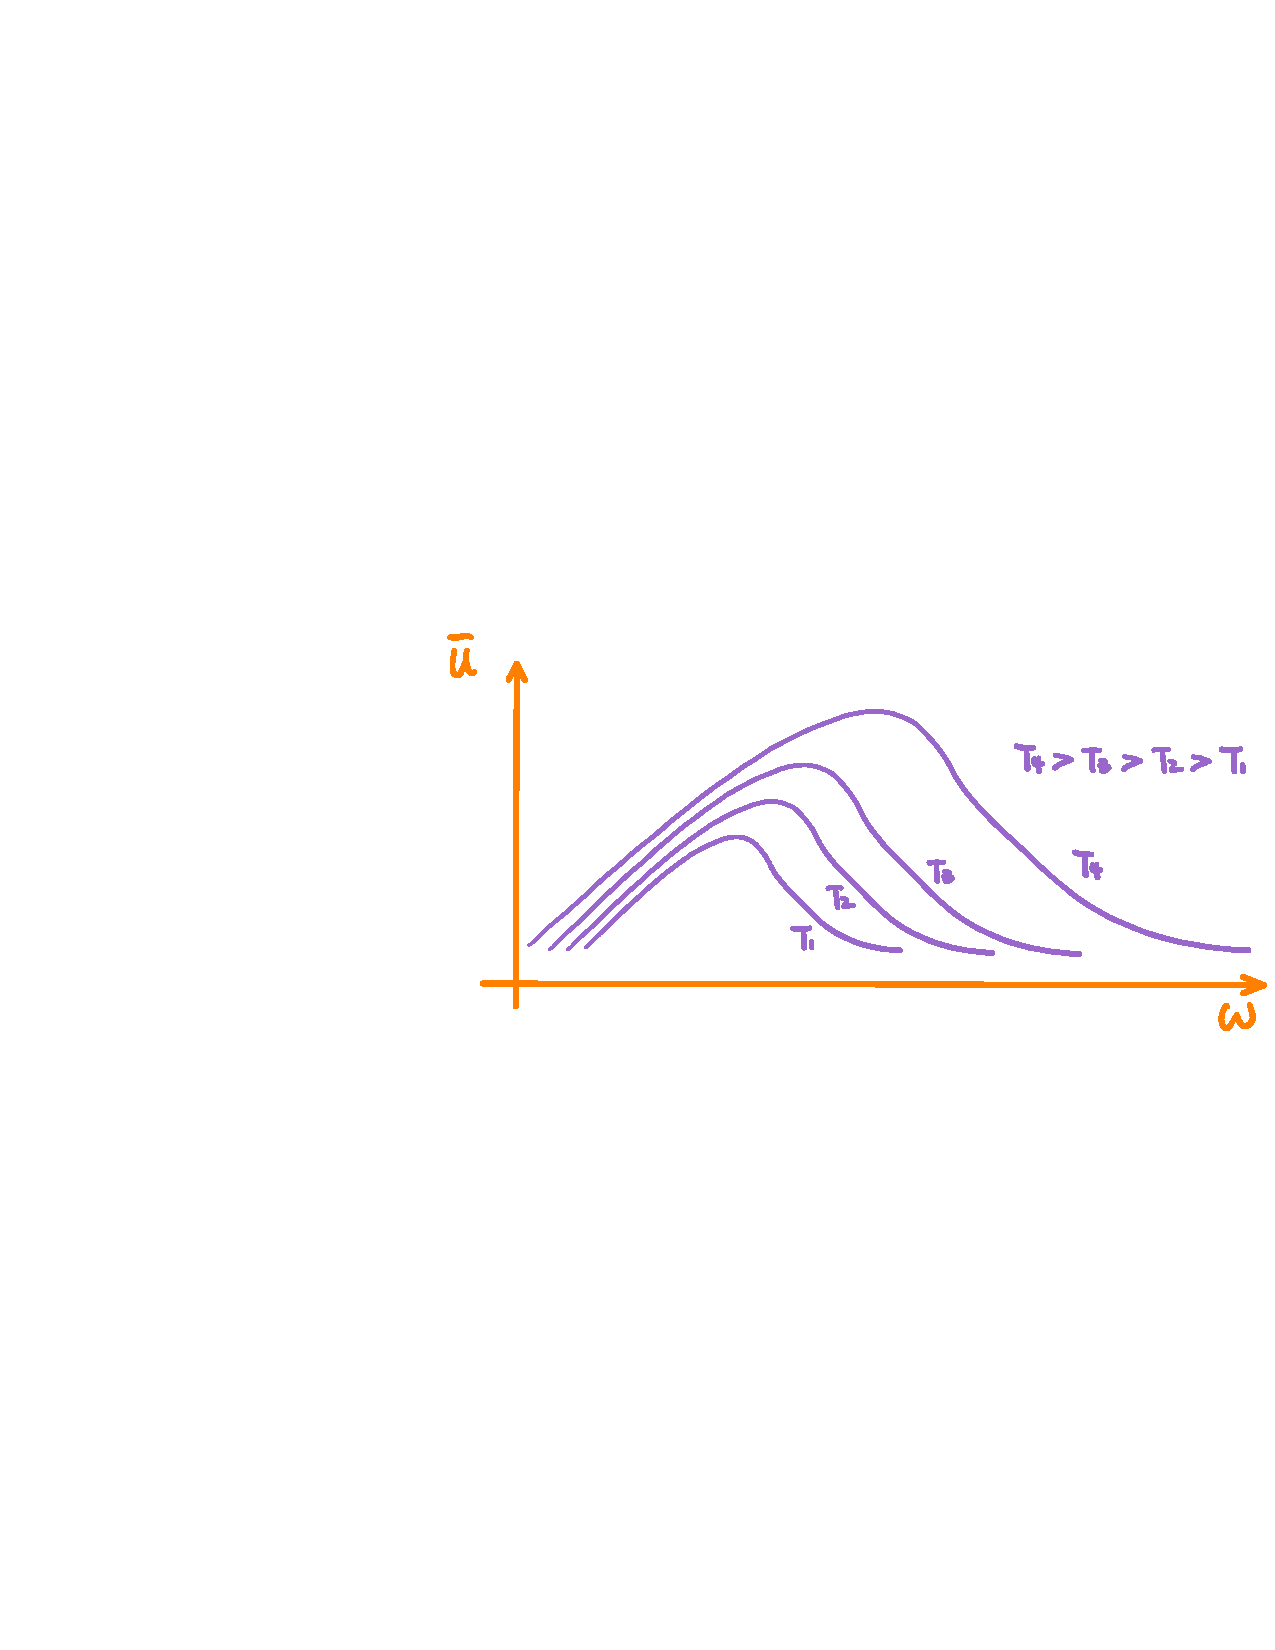
\includegraphics[scale=0.69]{Plank.pdf}\\
\text{\color{gray} Figure. Wein's Displacement Law\color{black}}
\end{center}
\vspace*{\fill}

\begin{center}
\begin{tabular}{rcl}
Courses Instructor & & Ratindranath Akhoury \medskip
\\
Notes Transcriber & & Jinyan Miao\medskip
\\
Text Editor & & Jinyan Miao \medskip
\\
Art Designers & & Wenyu Chen \\
 & & Jinyan Miao \bigskip
\end{tabular} \\
This text is prepared using the \TeX\ typesetting language. \\
Materials credit to the Department of Physics at the University of Michigan.\\
This work is licensed under a Creative Commons By-NC-ND 4.0 International License.  \\
\medskip

\includegraphics[scale=0.8]{cclisence.png}
\end{center}
\hfill\break

This text is intended as a supplemented class notes for students who are taking, or intend to take, Physics 406 at the University of Michigan. We assume that the reader has taken introductory physics courses, at least covering classical mechanics and introductory quantum physics. We will make use of some usual notation that were introduced in those courses.\\

In this text, some figures and materials credit to the text \textit{Fundamentals of Statistical and Thermal Physics}, by Frederick Reif, published by Waveland Press in 2009.\\

This text is edited by Jinyan Miao. The course Physics 406 in Winter 2022 is taught by Professor Akhoury at the University of Michigan - Ann Arbor.\ Except as permitted by Jinyan, no part of this text is allowed to be distributed. This text contains information obtained from authentic sources, but we cannot assume responsibility for the validity of all materials in this text or the consequences of their use. We have attempted to trace the copyright holders of all material reproduced in this text and apologize to copyright holders if permission to share in this form has not been obtained. If any copyright material has not been acknowledged please write and let us know. If you have any questions or concerns regarding this text, or if you find any typos in this text, please contact Jinyan through jmiu@umich.edu. 


\newpage
\setcounter{chapter}{0}
\chapter{Microcanonical Ensemble}
\section[Probability Theory Review]{\color{red}Probability Theory Review\color{black}}
Let $P_r$ denotes a discrete probability, we have $1\geq P_r \geq 0$, with $\sum_r P_r = 1$.\\

When we have large number of systems, discrete probabilities become continuous values, and here we get a probability distribution, $P(x)\, dx$ is the probability that the system lies in the state between $x$ and $x+ dx$. \\


In discrete probability $P_r$, given $f(r)$, the average of $f$is given by: $$\bar{f} = \sum_r f(r) P_r$$\\
In continuous probability $P(x)$, given $f(r)$, the average of $f$ is given by $$\bar{f} = \int_{-\infty}^\infty P(x) f(x)\, dx$$ \\

Binomial distribution plays a special role. Suppose one makes $N$ independent trials, the probability of a "hit" is $p$, and the probability of a "miss" is $q$, with $p+q = 1$. Then the probability of exactly $m$ "hits" in $N$ trials is given by the following:
$$P_m = \frac{N!}{m!(N-m)!}p^m q^{N-m}$$
and we have $\sum_m P_m = 1$.\\


For mean values of binomial distribution:
\begin{align*}
\bar m &= \sum_{m=0}^N mP_m = \sum_{m=0}^N \frac{N! m}{m!(N-m)!}p^mq^{N-m} \\
&= p\frac{\partial }{\partial p} \left(\sum_{m=0}^N \frac{N!}{m!(N-m)!}p^m q^{N-m} \right)\\ 
&= p\frac{\partial}{\partial p}(p+q)^N = Np(p+q)^{N-1}\\
&= Np
\end{align*}
\begin{align*}
\overline{m^2} &= \sum_{m=0}^N m^2 P_m \\
&= \sum_{m=0}^N \frac{N1}{m!(N-m)!}m^2p^mq^{N-m}\\
&= Np+(N^2-N)p^2
\end{align*}

The dispersion is the measure of how much is the deviation from the mean value:
$$(\Delta m)^2 = \overline{(m-\bar{m})^2} = \overline{m^2} - 2\bar{m}^2 + \bar{m}^2 = \overline{m^2} - \bar{m}^2 = \sqrt{Np(1-p)}$$

Fractional dispersion:
$$\frac{\Delta m}{\bar{m}} \approx \frac{\sqrt{N}}{N} \approx \frac{1}{\sqrt{N}} $$
Here we see that for very larger number of trials, one can approach the mean value. 
\newpage

\section[Macroscopic and Microscopic Descriptions of Physical Systems]{\color{red} Macroscopic and Microscopic Descriptions of Physical Systems\color{black}}

For systems with large number of particles, we will try to find a microscopic description for such system, one might want to assigning position $\vec{r}_i$ and momentum $\vec{p}_i$ for all the particles. If such system has $N$ particles, a phase space is the space of momenta and positions of the particles, which has $3N$ position coordinates, $3N$ momenta coordinates, and hence a $6N$ dimensional space. The state of each particle in the system is a point in this phase space. On the other hand, the macroscopic description of a system with large number of particles, say, number of particles $\geq \ee{23}$, uses the macroscopic variables such as $V$, $N$, $T$, and so on.\\

Thermodynamics describes the macroscopic relation between the macroscopic parameters of the system without any reference to microscopic properties, and statistical mechanics is the microscopic description of thermodynamics.\\

For each macroscopic description of a system, there is information missing about the microscopic state of the system. In other words, there can be many different microstates of the system that give the same macroscopic parameters of the system.\\


Consider there spins in a magnetic field. Spin up has energy $-\mu H$, and spin down has energy $+\mu H$. \\
The following are some of the microstates:
\begin{enumerate}[topsep=3pt,itemsep=-1ex,partopsep=1ex,parsep=1ex]
\item (up) (up) (up)
\item (up) (up) (down)
\item (down) (up) (up)
\item (up) (down) (up)
\item (down) (down) (up)
\item etc.
\end{enumerate}
For cases (2), (3), and (4), all have total energy $-\mu H$, they are microstates consisting of two ups and one down. If one fixes the macroscopic state by specifying the total energy, say $E_{total} = -\mu H$, we observe that there are three microstates that give the same macroscopic description. To generalize, when one specifies a macrostate, there is information missing about the microstate of such system. Many microstates will give the same macrostate. The sates correspond with a given macrostate are called the accessible states. In this example, only three microstates are accessible to the total energy $E_T = -\mu H$. This is where probability comes in to the description and hence irreversible problem. 

\newpage
\section[Accessible Microstates]{\color{red}Accessible Microstates\color{black}}
Ensemble is many copies of the system with the same macrostate but the microstates can be distributed among the various accessible states. Probability $p$ for a particular microstate $r$ is given by the following:
\begin{align*}
p(r) = \frac{\text{number of systems in this microstate}}{\text{total number of systems in the ensemble}}
\end{align*}
The question is how to assign the probabilities to the different accessible microstates. The criteria for assigning probabilities is that we want to maximize the missing information.\\

Suppose a particular event occurs with probability $p$. Let $I(p)$ be the missing information. Note that if the probability $p = 1$, we have $I(p) = 0$. Information is non-negative, so we have $I(p) \geq 0$ for all $p$. If there are two independent events with probabilities $p_1$ and $p_2$, then the joint probability\footnote{Joint probability is the likelihood of two events occurring together and at the same time.} of the two events is $p_1 \cdot p_2$. Hence we have $I(p_1\cdot p_2) = I(p_1) + I(p_2)$. Also, information measure is monotonic and continuous. The consequence of these can be generalized to the following:
$$I(p^{\frac{m}{n}}) = \frac{m}{n}I(p)$$
From continuity, we get that, for $0\leq p \leq 1$, and real $a$, we have $I(p^a) = a \, I (p)$. 
For such case, one solution is given by the following:
$$I(p) = -k\, \ln (p)$$
with Boltzman constant $k$. Note that choosing a different base for the logarithm function yields a different constant coefficient. \\

Now suppose we have a set of events labeled by integers $\{r \mid r\in R \subseteq \Z\}$, each occurring with probability $\{ p_r \mid r \in R\}$. We would want to find the expected amount of missing information in $N$ observation. Event $r$ occurs on the average $N\cdot p_r$ times, and the missing information content in $p_r$ is given by $-k \ln (p_r)$, so the average missing information per observation is given by the following:
$$I = \frac{-k \sum_r N p_r \ln p_r}{N} = -k \sum_r p_r \ln (p_r)$$
If the probability for each event is equal, and say there are $n$ events in total. $p_1 = p_2 = \cdots  \coloneqq p$. Then we can write the following:
$$I = -k \sum_r \frac{1}{n} \ln\left(\frac{1}{n}\right) = k\ln(n)$$
\newpage

Consider an isolated system in equilibrium\footnote{System in equilibrium implies that the macroscopic parameters for such system do not change in time}. We would like to find the probability distribution that we can assign to the microstates in an ensemble describing the isolated system. Denote the missing information for such system as $S$, we want to maximize $S/k = -\sum_r p_r \ln (p_r)$ under the constraint $\sum_r p_r = 1$ for some constant $k$ by using the methods of Lagrange multiplier. 

\begin{align*}
\frac{\pd}{\pd p_i}\left( -\sum_r p_r \ln(p_r) - \alpha \sum_r p_r\right) &= 0\\
-\sum_r \delta_{ir} \ln( p_r) - \sum_r p_r \frac{\delta_{ir}}{p_r} - \alpha\sum_r \delta_{ir} &= 0\\
-\ln(p_r) - 1 - \alpha &= 0\\
\ln(p_r) &= -a-\alpha \\
p_r &= e^{-1-\alpha}\\
\end{align*}
with $\sum_r e^{1-\alpha} = 1$, we get $e^{-1-\alpha} = \frac{1}{n}$
Hence we conclude that:
$$p_r = \frac{1}{n}$$
Hence we see that, an ensemble describing isolated system in equilibrium is one in which all microstates are equally probable, such ensemble is called a microcanonical ensemble.\\
\hfill\break

Now consider a system with a large number $N$ of particles, in a volume $V$, and energy of this system is given in between $E$ and $E+ \delta E$, with $\delta E$ being small, that is, assume $\delta E << E$. \\

Specifying the state of a moving particle in $1$-dimension can be done by giving the the position $q$ and momentum $p$ of the particle. Consider a $2$-dimensional phase space of $p$ and $q$, with $p$ on the y-axis and $q$ on the x-axis. Each point in such phase space is a state for a particle. To count the number of states in the phase space, one can divide the phase space into small regions $\delta p$ with $\delta q$. Classically, we say $\delta p \cdot \delta q \approx h_0$. In quantum mechanics, from uncertainty principle, we have $h_0 \approx h$, the Plank's Constant. The number of microstates is given by the region of the entire phase space (area, volume, $\cdots$) divided by $h_0$ (for area). \\


\example\\
For Harmonic Oscillation in $1$-dimension, the total energy is given by the following:\\
$$\frac{1}{2}mv^2 + \frac{1}{2}kq^2 = E$$
with $q$ being position. Rearranging we get the following:
\begin{align*}
p^2 + m^2 \omega^2 q^2 = 2mE \qquad\qquad\text{with }\omega = \sqrt{\frac{k}{m}}
\end{align*}
\begin{center}
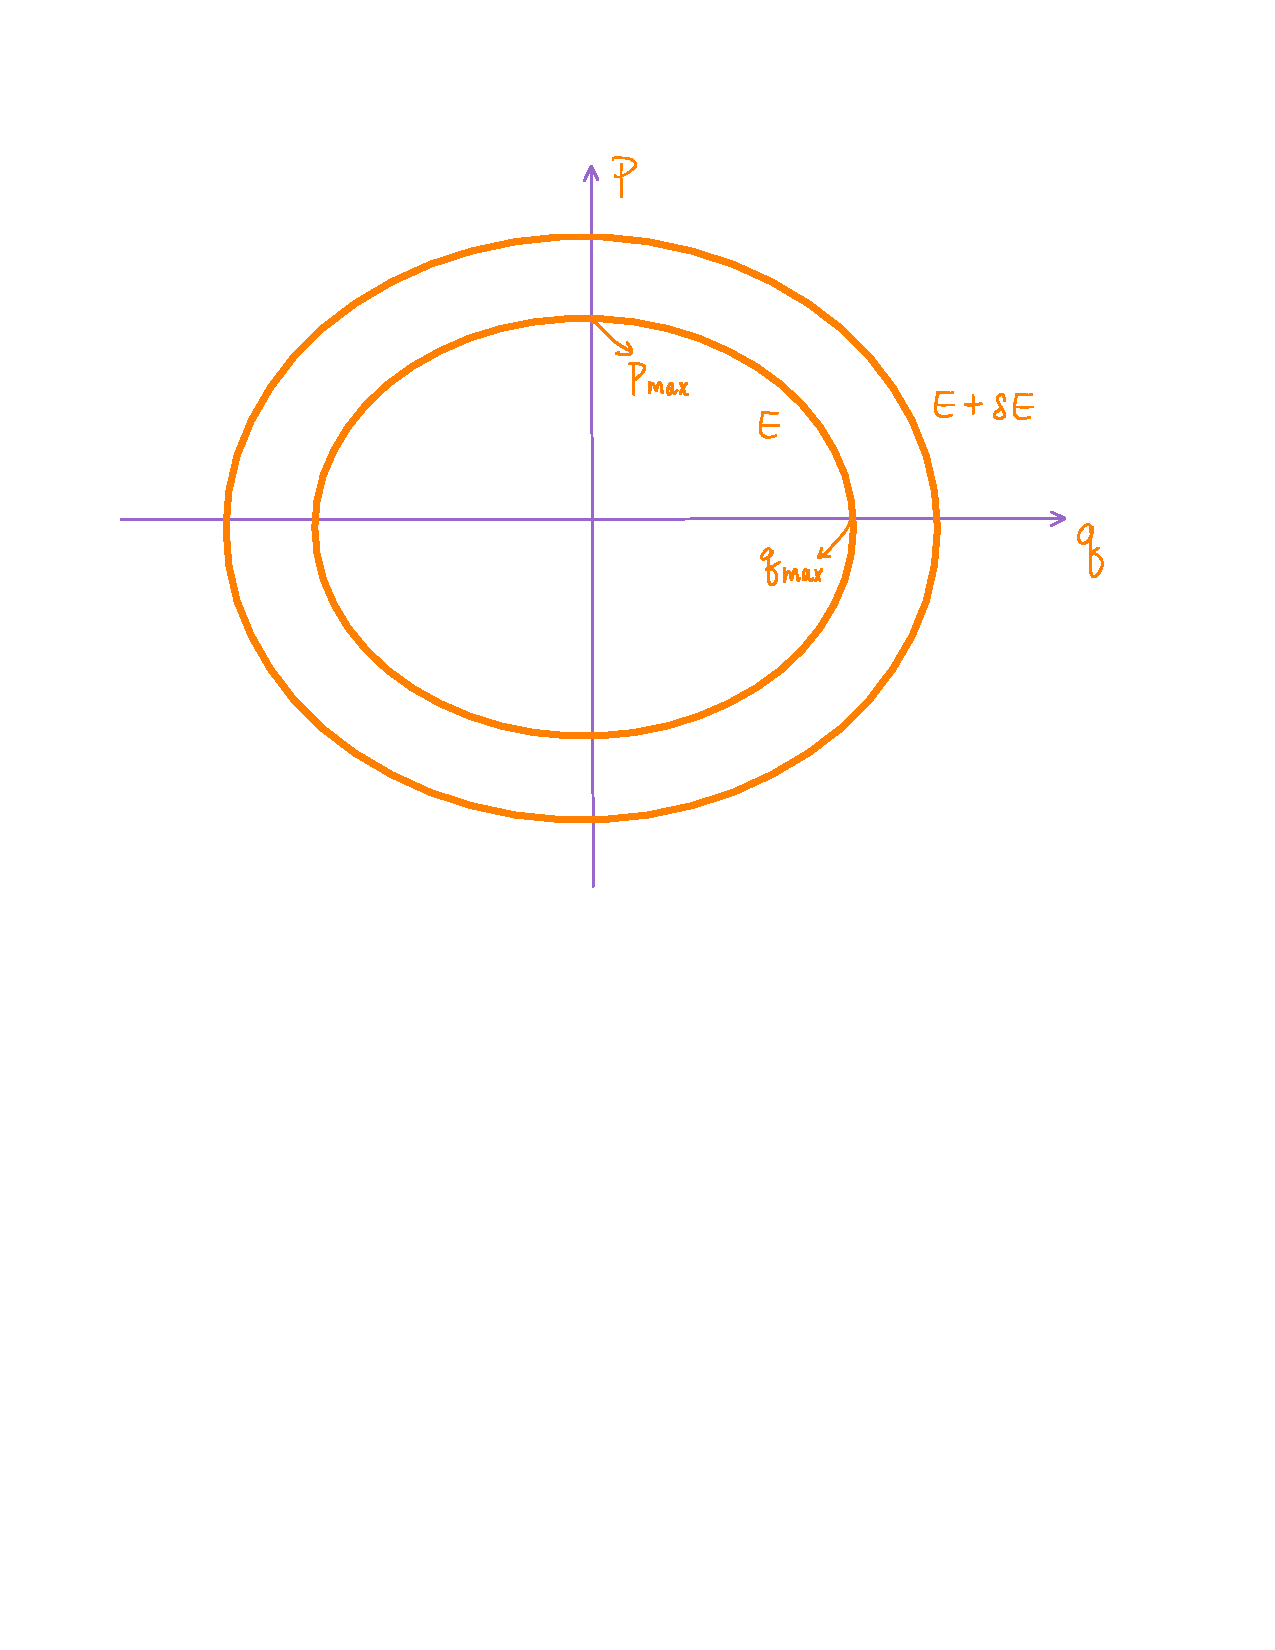
\includegraphics[scale=0.5]{pqPhaseSpace.pdf}
\end{center}
Let $\Phi(E)$ be the number of microstates with energy less than or equal to $E$. Let $\Omega(E)$ be the number of microstates with energy with energy between $E$ and $E+\delta E$. Here we get the following:
$$\Phi(E) = \frac{\pi p_{max} \cdot q_{max}}{h_0} = \frac{\pi (2mE)}{h_0(m\omega)} = \frac{E}{\frac{h_0}{2\pi} \omega}$$
For $\delta E << E$, we get the following:
$$\Omega(E) = \Phi(E+\delta E) - \Phi(E) = \frac{\partial \Phi}{\pd E}\delta E = \frac{\delta E}{\frac{h_0}{2\pi}\omega}$$

\hfill\break
Let $f$ be the degrees of freedom, $f$ momenta and $f$ coordinates. The dimension of phase space is them $2f$. Hence the volume of each cell in such phase space is given by: $$\delta q_1 \cdot \delta q_2 \cdot \cdots \cdot \delta q_f \cdot \delta p_1 \cdot \delta p_2\cdot \cdots \cdot \delta p_f = h_0^f$$


\example\\
For $1$-dimensional harmonic oscillation, with quantum theory, we can write:
$$E = \left(n+\frac{1}{2}\right) \hbar \omega$$
with $n\in \N$ being the energy level. A microstate is completely specified by a given $n$. Spacing between energy levels is $\hbar \omega$. Assuming $\delta E > \hbar \omega$, the number of microstates between $E$ and $E+ \delta E$ is then given by the following: 
$$\Omega(E) = \frac{\delta E}{\hbar \omega}$$
Comparing with what we get above for classical description of $1$-dimensional harmonic oscillation, the classical and the quantum description agree for $h_0 \approx h$, with $h$ being the Plank's Constant. \\


\example\\
We would like to find the number of accessible microstates for a monatomic ideal gas of $N$ particles in a volume $V$. Note that there is no interaction between particles, so the total energy of such system is given by the following:
$$E = \sum_{i=1}^N \frac{||\vec{p}_i||^2}{2m}$$ which is the sum of the kinetic energy of all particle. Hence we get a constraint:
$$\sum_{i=1}^N (p_{ix}^2 + p_{iy}^2 + p_{iz}^2) = 2mE$$
For $3$-dimensional, suppose there are $N$ particles, each with $3$ degrees of freedom, so total of $3N$ degrees of freedom. The volume of each elementary region in the phase space is given by:
$$dq_1\cdot dq_2 \cdot \cdots \cdot dq_{3N}\cdot dp_1\cdot dp_2\cdot \cdots \cdot dp_{3N} = (h_0)^{3N}$$
Then we have: 
\begin{align*}
\Phi(E) &= \frac{1}{(h_0)^{3N}}\int dq_{1} \cdots dq_{3N} dp_1 \cdots dp_{3N}\\
&= \frac{1}{(h_0)^{3N}} \int dq_1 \cdot dq_2 \cdots \cdot dq_{3N} \int dp_1 \cdot dp_2 \cdots \cdot dp_{3N}
\end{align*}
Integrating over $dq_{1} \cdots dq_{3N}$ under the volume constraint $V$ gives $V^N$, and integrating over $ dp_1 \cdot dp_2 \cdots \cdot dp_{3N}$ under the constraint $\sum_{i=1}^N (p_{ix}^2 + p_{iy}^2 + p_{iz}^2) = 2mE$, which is a equation for a $3N$-dimensional sphere, gives $k(\sqrt{2mE})^{3N}$ for some constant $k$. Hence we can write:
$$\Phi(E) = \frac{k}{h_0} V^N E^{3N/2} \qquad \qquad \Omega(E) = \Phi(E + \delta E) - \Phi(E) \approx \frac{\partial \Phi(E)}{\partial E} \delta E = \frac{k}{h_0} V^N E^{\frac{3N}{2}-1} \delta E$$
The approximation for $\Omega(E)$ is obtained through Taylor Expansion of $\Phi$. \\

\example\\
For a particle trapped between two walls. Let $L$ be the distance between two walls, we get: $$E_n = \frac{\pi^2 \hbar^2}{2m} \left(\frac{n^2}{L^2}\right)$$ for $n \in \N$ being the quantum number. One can specify the microstate by giving $n$. \\
For a particle in a $3$-dimensional box, which dimension is given by $L_x\times L_y\times L_z$, 
$$E = \frac{\pi^2 \hbar^2}{2m}\left(\frac{n_x^2}{L_x^2} + \frac{n_y^2}{L_y^2}+ \frac{n_z^2}{L_z^2}\right) $$
where $n_x$, $n_y$ and $n_z$ are quantum numbers. One can specify the microstate by giving $n_x$, $n_y$, and $n_z$. \\
\newpage

A microcanonical ensemble describes an isolated system in equilibrium in which all microstates are equally probable. We use $\Omega(E)$ denote the number of microstates with energy between $E$ and $E+\delta E$, where $\delta E$ is greater than the amount of energy required to go between quantum levels in quantum theory. In the following we want to investigate how $\Omega(E)$ depends on $E$ for a system with high degrees of freedom. We will show in fact, by estimation, $\Omega(E) \propto E^f$ where $f$ is the number of degrees of freedom. In the following we denote $\Phi(E)$ as the number of microstates with energy less than or equal to $E$.\\


Consider a system of large number $(\geq 10^{23})$ degrees of freedom, and particles in such system are considered to be indistinguishable and non-interacting. Each degree of freedom, which could be considered as a particle moving in only one single direction, has its own energy levels. Let $\epsilon$ denote the energy of such particle, and $\Delta \epsilon$ denote the amount of energy required to go from one energy level to the consecutive one. For the entire system. Let $\Delta E$ denote the energy spacing between levels, with $\delta E > \Delta E$. Typically, we can write $\epsilon = \frac{E}{f}$. First note that, for $\delta E <<E$, we can write:
\begin{align*}
\Omega(E) = \Phi(E+\delta E) - \Phi(E) \approx \frac{\partial \Phi(E)}{\partial E}\delta E \tag{1}
\end{align*}
If two particles each has $m$ microstates with energy level less than $\epsilon$, then the total microstates in the system consisting of the two particles only, with energy level less than $E = 2\epsilon$, is $n^2$. With such argument, we can write the following:
$$\Phi(E) = \left(\Phi(\epsilon)\right)^f$$
Hence we can rewrite equation (1) as the following:
\begin{align*}
\Omega(E) \approx \frac{\partial \Phi(E)}{\partial E}\delta E =  (f)(\Phi(\epsilon))^{f-1}\left(\frac{\partial \Phi(\epsilon)}{\partial \epsilon}\frac{\partial \epsilon}{\partial E}\right) \delta E \tag{2}
\end{align*}
Notice that we also have:
$$\Phi(\epsilon) = \frac{\epsilon}{\Delta \epsilon} \quad \Rightarrow \quad \frac{\partial \Phi(\epsilon)}{\partial \epsilon} = \frac{1}{\Delta \epsilon}\qquad\qquad\qquad\qquad\qquad\qquad \epsilon = \frac{E}{f}\quad \Rightarrow \quad \frac{\partial \epsilon}{\partial E} = \frac{1}{f}$$
Hence equation (2) can be rewritten as the following:
$$\Omega(E)  = (f)(\Phi(\epsilon))^{f-1}\left( \frac{1}{\Delta \epsilon}\frac{1}{f}\right) \delta E = (\Phi(\epsilon))^{f-1} \frac{\delta E}{\Delta \epsilon}$$
One can show that $\Phi(\epsilon) \propto \epsilon^\alpha$ with $\alpha$ of order $1$, then we can write: 
$$\Phi(\epsilon) = \Phi(E/f) \propto E \qquad \Rightarrow \qquad \Omega(E) \propto E^{f-1} \frac{\delta E}{\Delta \epsilon}$$
Here we observe that we have: 
$$\ln(\Omega(E)) = (f-1)\ln (E) + \ln \left( \frac{\delta E}{\Delta \epsilon}\right) + constant$$
so for a good approximation, we have
$$\ln(\Omega(E)) \approx f\ln(E) + constant$$
or we have 
$$\Omega(E) \propto E^f$$
when $f$ is large enough. Here we see that $\Omega(E)$ is a rapidly varying function of $E$.

\newpage
\chapter{Mathematics in Thermodynamics}

\section[Thermal and Mechanical Interactions]{\color{red}Thermal and Mechanical Interactions\color{black}}
Now we will introduce interactions between subsystems of an equilibrium system. \\There are two types of interaction: (1) the thermal interaction and (2) the mechanical interaction. \\

\example\\
Consider an isolated system, denoted as $A^0$, composed of two parts, $A$ and $A'$, which are themselves not isolated. The systems $A$ and $A'$ are connected by a thermally conducting movable wall. Here we can specify the macrostate of $A^0$, with $N,\ V,\ E,\ $ etc. for both $A$ and $A'$. \\
\begin{center}
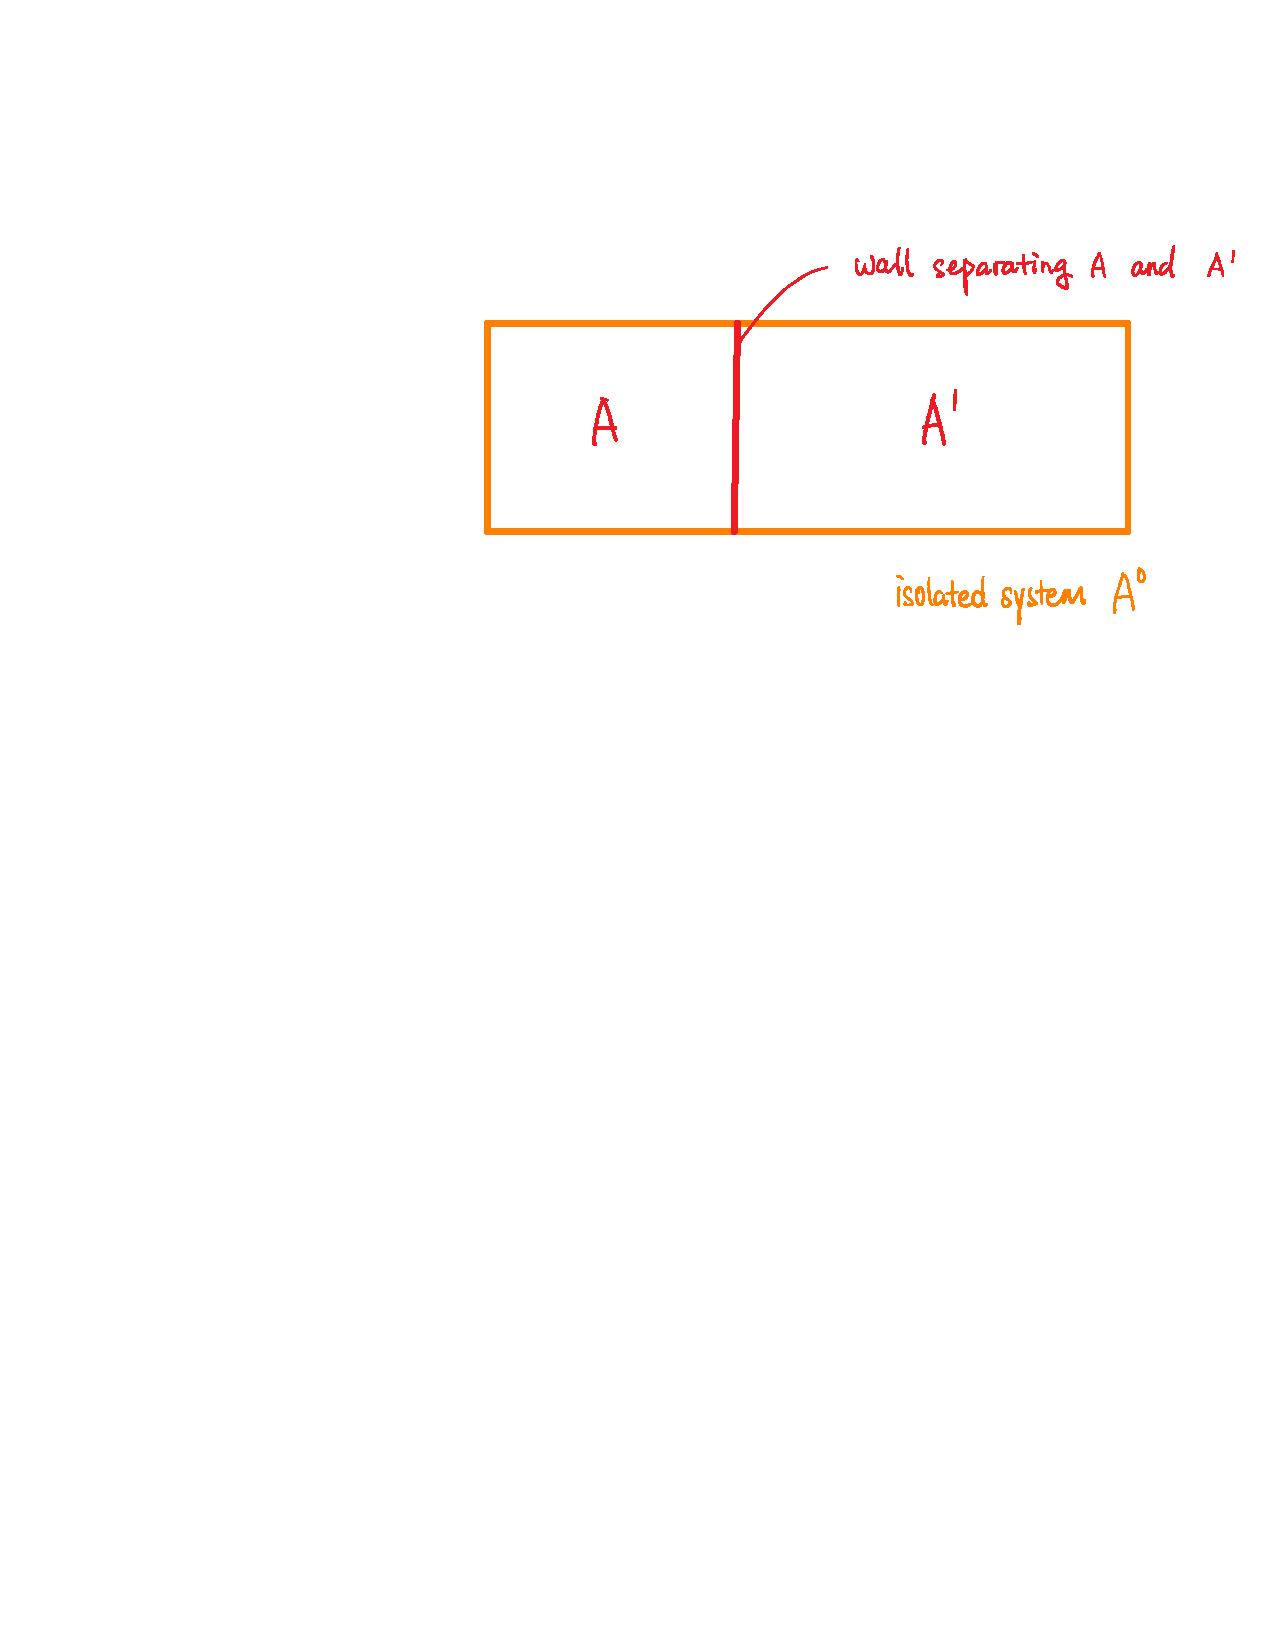
\includegraphics[scale=0.5]{interaction.pdf}
\end{center}

Note that energy is a function of external parameters. As we saw from the last example, particle in a $3$-dimensional box have $E\propto \frac{n_x^2}{L_x^2} +\frac{n_y^2}{L_y^2}+ \frac{n_z^2}{L_z^2}$, where $L_x, L_y, L_z$ are external parameters. \\

In a macroscopic description, it is always useful to distinguish the two types of interaction, which are the thermal and mechanical interactions. For thermal interaction, external parameters of $A$ and $A'$ are fixed, but mean energies of $A$ and $A'$ will change. The mean energy transferred from one system to the other, say $A$ to $A'$, as a result of thermal interaction, and the energy transferred is called the heat. For mechanical interaction, external parameters of $A$ and $A'$, such as position of the wall separating $A$ and $A'$, will change, and one does work on the other. In this way, the mean energies of $A$ and $A'$ also change. \\

Also note that, when external parameters are kept fixed, then the energy for each probable microstate $E_r$ is fixed. If $\bar{E} = \sum_r p_r E_r$ changes, with $E_r$ being fixed, then we know that $p_r$ must have been changed.   \\

Microscopically, consider a single particle in a $1$-dimensional box.\\
First we consider a purely thermal interaction. 
\begin{center}
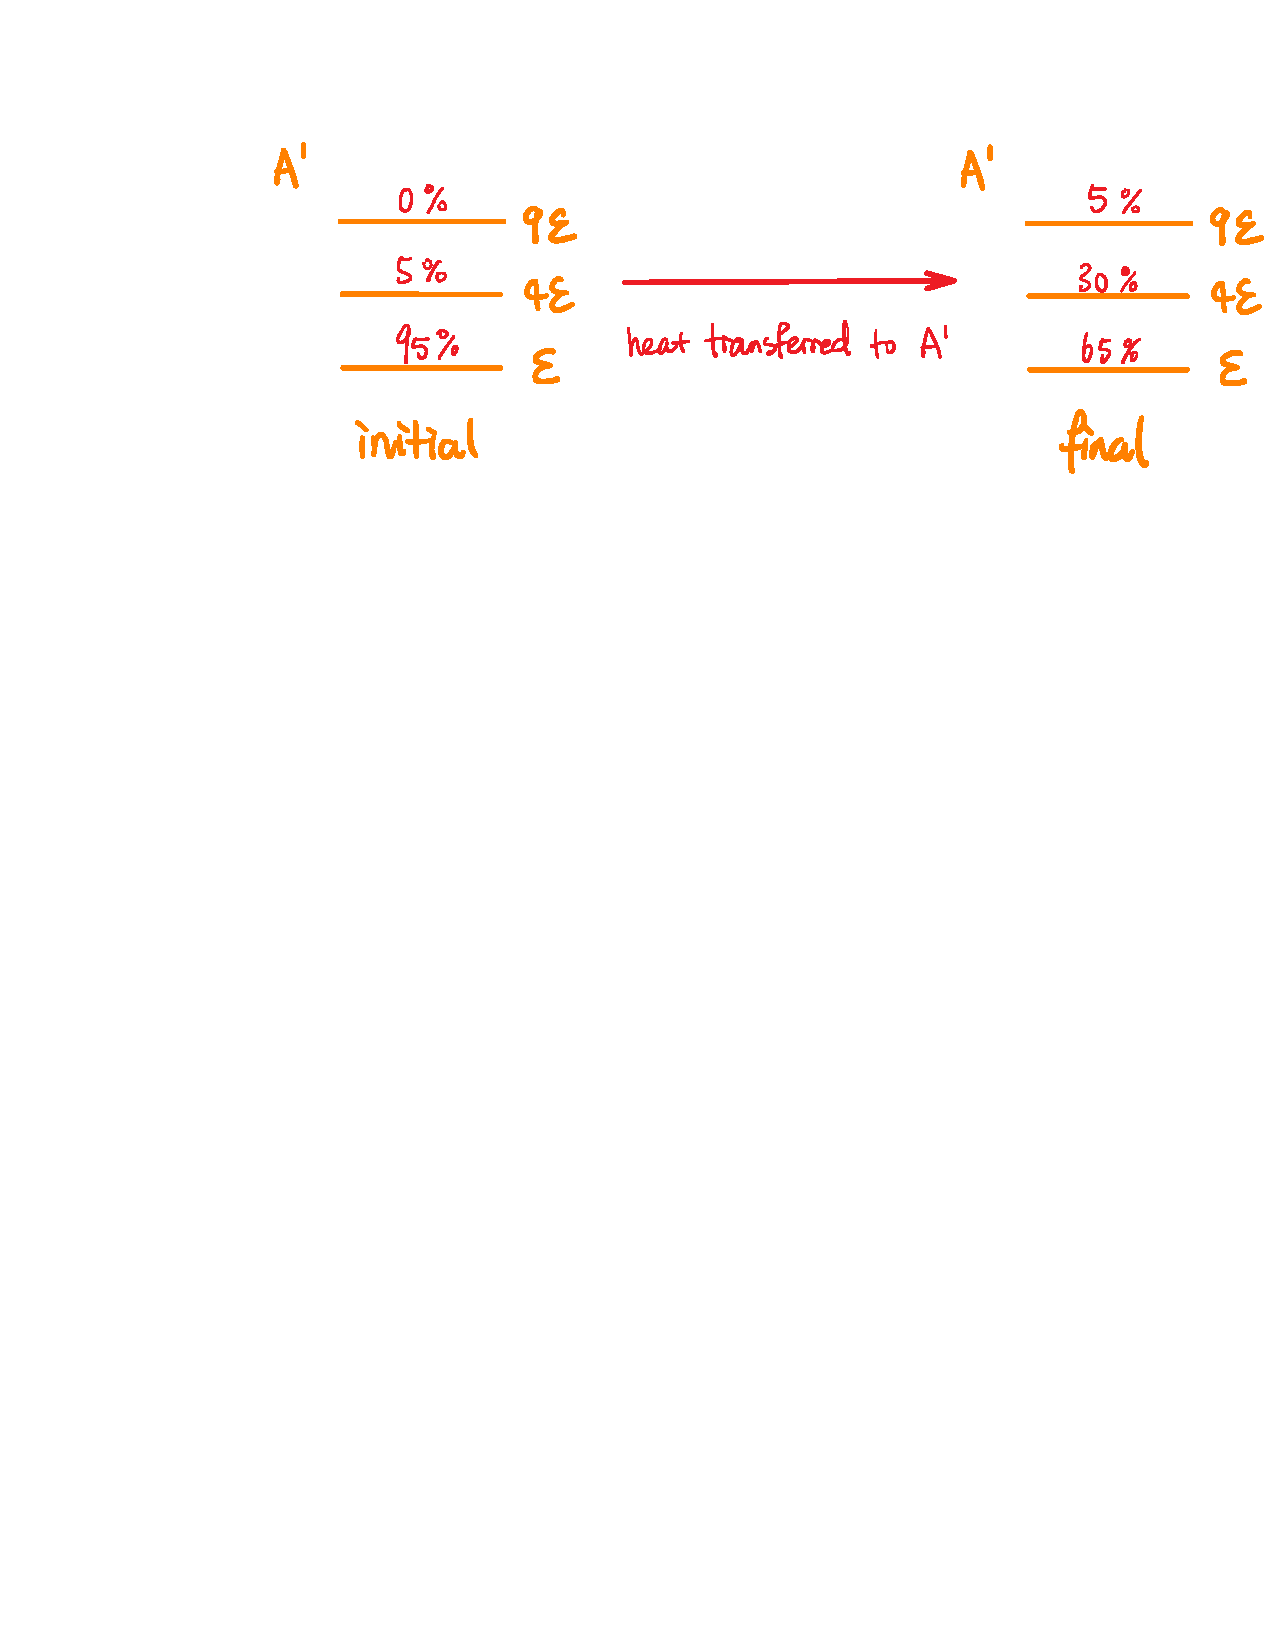
\includegraphics[scale=0.5]{thermalInteraction.pdf}
\end{center}
Here we can write:
$$\bar{E}_{intial} = 0.95 \epsilon + (0.05)(4\epsilon) = 1.15\epsilon$$
$$\bar{E}_{final} = 0.65 \epsilon + (0.3) (4\epsilon) + (0.05)9\epsilon = 2.3\epsilon$$
$$\text{Energy transferred: } Q = \Delta \bar{E} = 2.3\epsilon - 1.15\epsilon = 1.15\epsilon$$
Note that $E + E' = E^0$ is being fixed, where $E^0$ is the total energy of the system, $E,E'$ are energies for $A$ and $A'$, respectively. \\

Now consider a purely mechanical interaction. Here energy levels change. Say we compress $A'$ and make the wall between $A$ and $A'$ thermally insulating. As we do that, since the box of $A'$ is smaller, then the external parameters for $A'$ change. We compress $A'$ slowly such that $E^0$ is still fixed. 
\begin{center}
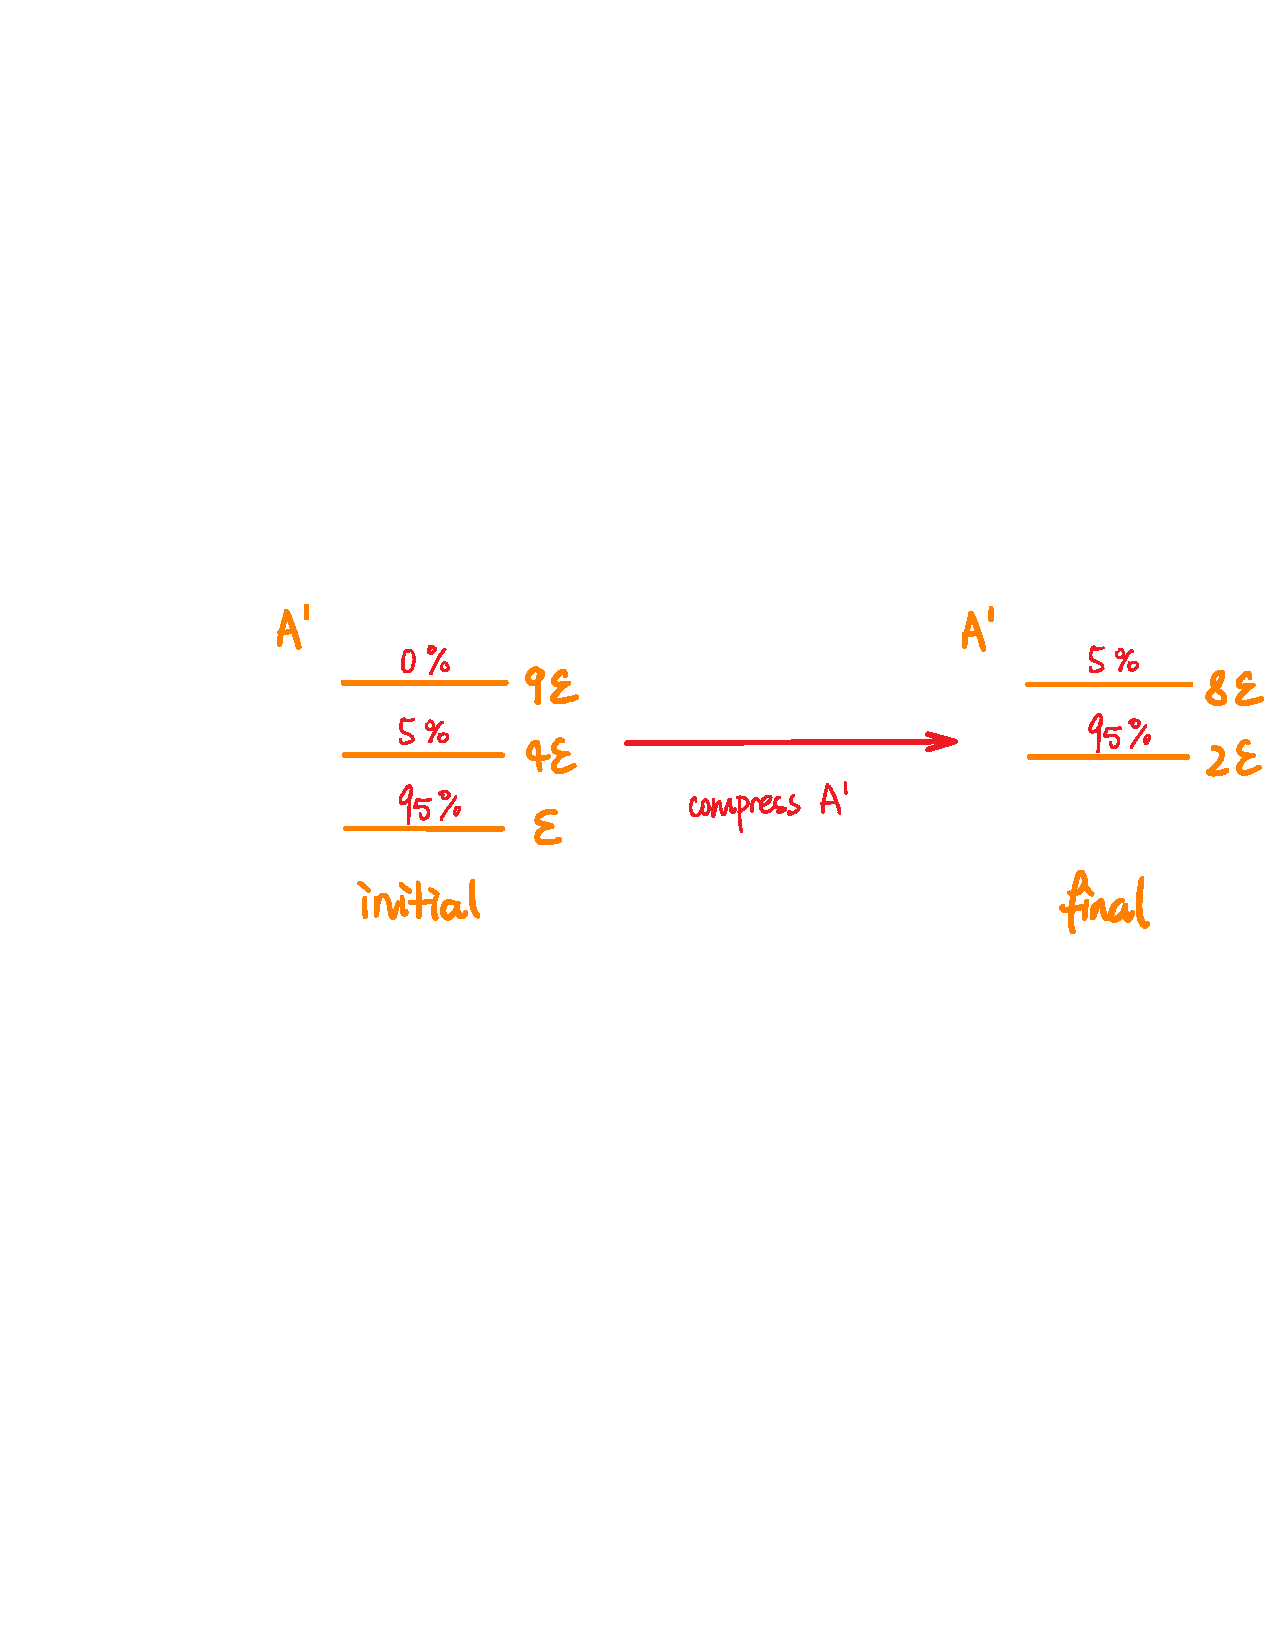
\includegraphics[scale=0.5]{mechanicalInteraction.pdf}
\end{center}
Now we can write:
$$\bar{E}_{initial} = 1.15\epsilon$$
$$\bar{E}_{final} = 2.3\epsilon$$
$$\text{Work done by }A' \text{ is given by }W = -\Delta \bar{E} = -1.15\epsilon$$


For a general interaction, both the external parameters change and the wall is thermally conducting, the division of energy transfer to heat and work is not so straightforward. Now consider a general interaction. That is, the wall of partition is thermally conducting and is movable. The average energy is given by:
$$\bar{E} = \sum p_r E_r$$
where both $p_r$ and $E_r$ might change. Now the division of energy transfer into heat and work is not well defined, in fact, they are process dependent. Energy is a function of external parameters, denoted as $E_r(x_1,x_2,\cdots, x_n)$, where $x_1,x_2,\cdots, x_n$ are external parameters, including volume, length, mechanic or electric field, and so on. Before interaction, we write $\bar{E} = \sum_r p_r E_r$. During interaction, $p_r$ could be changed to $p_r + \delta p_r$, and the external parameters would change, hence we have $E_r$ changes to $E_r + \delta E_r$, so the change in average energy is given by the following:
\begin{align*}
\overline{\Delta E} = \sum_r (p_r +\delta p_r)(E_r+\delta E_r) - \sum_r p_r E_r \tag{1}
\end{align*}
Now consider an infinitesimal change, which implies we could ignore the $\delta p_r \cdot \delta E_r$ terms, here we can rewrite equation (1):
\begin{align*}
\overline{\Delta E} = \sum_r \delta p_r E_r + \sum_r p_r \delta E_r \coloneqq \dbar Q -\dbar W
\end{align*}
here $\dbar W$ and $\dbar Q$ are not exact differentials. That is, we write:
$$\int_a^b \dbar W \neq W(b)-W(a)$$ 
Instead, $\int_a^b \dbar W$ is path dependent. Nevertheless, we will see that $\int_i^f \overline{ \Delta E} = E_f - E_i$, that is, $E$ depends only on endpoints, not the path, but both $\int_i^f \dbar Q$ and $\int_i^f \dbar W$ are both path dependent. \\


First, for $\sum_r p_r \delta E_r = -\dbar w$, as $E_r$ is a function of $x_1,x_2,\cdots, x_n$, we have:
\begin{align*}
\delta E_r = \sum_{\alpha=1}^n \frac{\partial E_r}{\partial x_{\alpha}}dx_{\alpha} \qquad \Rightarrow \qquad -\dbar W = \sum_r p_r \left(\sum_{\alpha} \frac{\partial E_r}{\partial x_{\alpha}}dx_{\alpha}\right) = \sum_{\alpha}\sum_r\left( p_r\frac{\partial E_r}{\partial x_{\alpha}}\right)dx_{\alpha}
\end{align*}
Hence we can define the generalized force as the following: 
$$\bar{X}_{\alpha} = -\sum_r p_r \frac{\partial E_r}{\partial x_{\alpha}} = -\frac{\partial \bar{E}}{\partial x_{\alpha}}$$
It follows that we can write: 
$$\dbar W = \sum_{\alpha} \bar{X}_{\alpha} dx_{\alpha}$$
$\bar{X}_{\alpha}$ is called the generalized force associated with the parameter $x_{\alpha}$. \\
Note that $\bar{X}_{\alpha}$ is a well defined macroscopic quantity.\\

Now $\dbar W = \sum_{\alpha} \bar{X}_{\alpha} dx_{\alpha}$ makses sense both microscopically and macroscopically. \\
To get a better sense of it, here we consider examples as the followings:\\

\example\\
Let $x_{\alpha}$ be volume. Then we have:
$$\bar{X}_{\alpha} = -\frac{\partial \bar{E}}{\partial V} = \bar{p} = \text{pressure}$$
Hence we can write $\dbar W = \bar{p}\, dV$. \\

Instead, if we have $x_{\alpha}$ being the length of a wire, then we have:
$$\bar{X}_{\alpha} = -\frac{\partial \bar{E}}{\partial l} = -\bar{T} = \text{tension}$$
Hence we can write $\dbar W = \bar{T}\, dV$.

\newpage
\section[Energy in Finite Quasi-static Process]{\color{red} Energy in Finite Quasi-static Process\color{black}}

\begin{thm}[Finite Quasi-static Process]
In this process, the system stays close to equilibrium at all times.\\ For such a process, the work done is given by: 
$$W \coloneqq \int \dbar W = \int \sum_{\alpha} \bar{X}_{\alpha} dx_{\alpha}$$
Then we write:
$$Q \coloneqq \overline{\Delta E} + W$$
In general, both $Q$ and $W$ depend on the process, but $\overline{ \Delta E} = E_f - E_i$ depends only on the initial and final states, being path independent. In particular, $d\bar{E}$ is exact differential.
\end{thm}

Adiabatic process is a Quasi-static process for which $\dbar Q = 0$, so we would write $Q= 0 $. \\

\example\\
If the only external parameter is $V$, the generalized force is then $p$. Any point on the $pV$-diagram specifies an equilibrium macrostate. Work done during a Quasi-static process is area under the curve, which depends on the process. \\

\example\\
We know that $\int_i^f dE = \int_i^f \dbar Q - \int_i^f \dbar W$, here we can write:
$$E_f - E_i = Q_{i\to f} - W_{i\to f}$$
For an Finite Quasi-static adiabatic process, we then have:
\begin{align*}
E_f - E_i = -W_{i \to f} = -\int p\, dV
\end{align*}

\hfill\break
More generally, $Q_{i\to f} = E_f - E_i + W_{i \to f}$. Here $E_f - E_i$ is measured mechanically in adiabatic process, and $W_{i \to f}$ is measured in process of interest.\\


Now consider a isolated system of equilibrium $A^0$, divided into two subsystems $A$ and $A'$, each with energy $E$ and $E'$ respectively, with $E^0 = E+E'$ being the total energy of $A^0$. Here $E^0$ is fixed as $A^0$ is an isolated system. Since $E^0$ is fixed, we take $E$ to be the only independent variable, and $E' \coloneqq E^0 - E$. The energy here is a function of both external $x_1,x_2,\cdots, x_n$ and internal parameters $y_1,y_2,\cdots, y_n$. Originally $A$ and $A'$ were separated by some constraint, now we remove the constraint between them and allow them to interact, in terms of both heat transfer and work. After interaction, the number of states accessible to the system increases. The most likely values of the internal parameters $y_1,y_2,\cdots,y_n$ after interactions are those that maximize missing information, here we denote the missing information as $\Omega(y_1,y_2,\cdots, y_n)$.\\

Consider first a purely thermal interaction, let $\Omega^0$ be the number of microstates accessible to $A^0$. Let $\Omega(E)$ be the number of states accessible to $A$, and $\Omega'(E')$ be the number of states accessible to $A'$. With energy for $A$ between $E$ and $E+\delta E$.
Here we have:
$$\Omega^0(E^0) = \Omega(E) \cdot \Omega' (E')$$
Recall that $\Omega(E)$ is a rapidly increasing function of $E$ as $E$ increases, with $\Omega(E) \propto E^f$ with $f$ being the degrees of freedom. $\Omega'(E') = \Omega'(E^0-E)$ is a rapidly  decreasing function of $E$ as $E $ increases. So the product will have a very sharp maximum. To maximize missing information, we want to maximize $\Omega^0(E^0)$. 
\begin{align*}
 \ln \Omega^0(E^0) = \ln \Omega(E) + \ln \Omega' (E')
\end{align*}
we have:
$$\frac{\partial \Omega^0(E^0)}{\partial E} = 0 \text{ at the maximum}$$
hence it follows that:
\begin{align*}
\frac{\partial }{\partial E}\ln \Omega(E) + \frac{\partial }{\partial E}\ln \Omega'(E') = 0 = \frac{\partial}{\partial E} \ln \Omega(E) - \frac{\partial }{\partial E'}\ln \Omega'(E') \tag{T}
\end{align*}
Here maximizing the missing information requires to find the condition that maximize $\Omega^0$. In such case, the two subsystems, with the new $E$ and $E'$ that maximize $\Omega^0$, is in equilibrium. Then here we have a way to define the temperature of the system $A^0$.
Rearranging equation (T) we get:
\begin{align*}
\frac{\partial }{\partial E}\ln \Omega(E) = \frac{\partial }{\partial E'}\ln \Omega'(E')
\end{align*}

Now we define:
\begin{align*}
\beta(E) \coloneqq \frac{\partial}{\partial E}\ln (\Omega(E))\qquad\qquad\qquad\beta'(E') \coloneqq \frac{\partial}{\partial E'}\ln (\Omega'(E'))
\end{align*}
At equilibrium where $E = \widetilde{E}$, we get the following:
\begin{align*}
\beta(\widetilde{E}) = p'(E_0-\widetilde{E})
\end{align*}
this property defines the temperature of the system:
$$T \coloneqq \frac{1}{k\beta}$$
with some convenient constant $k$. Now we can defined missing information as $$S \coloneqq k\ln(\Omega)$$ 
so $\beta = \frac{1}{k}\frac{\partial S}{\partial E}$, or we can write $\frac{1}{T} = \frac{\partial S}{\partial E}$. \\


In equilibrium thermodynamics, temperature is defined by $T^{-1} =\frac{\partial S}{\partial E}$, where $S$ is called the entropy. This allows us to define $S =k\ln(\Omega)$ being the entropy of the system. \\

Now we will investigate some properties of the given definitions. \\
Expand $\ln(\Omega(E))$ around $E = \widetilde{E}$, we can write the following:
\begin{align*}
\ln(\Omega(E)) &= \ln(\Omega(\widetilde{E})) + \left.\frac{\partial}{\partial E}\ln(\Omega(E))\right|_{E=\widetilde{E}} \Delta E + \left.\frac{1}{2}\frac{\partial^2}{\partial E^2}\ln(\Omega(E))\right|_{E=\widetilde{E}} (\Delta E)^2 + \cdots \\
&= \ln(\Omega(\widetilde{E})) + \beta(\widetilde{E}) \Delta E - \frac{1}{2}\lambda(\widetilde{E})(\Delta E)^2 + \cdots\\
\end{align*}
with $\lambda(\widetilde{E}') \coloneqq -\left.\frac{\partial^2}{\partial E^2}\ln(\Omega(E)) \right|_{E = \widetilde{E}}$. Let $\widetilde{E}'\coloneqq E^0 - \widetilde{E}$, similarly, we get the following:
\begin{align*}
\ln(\Omega'(E')) = \ln(\Omega'(\widetilde{E}')) - \beta'(\widetilde{E}') \Delta E - \frac{1}{2}\lambda'(\widetilde{E}') (\Delta E)^2
\end{align*}
Here we get:
\begin{align*}
\ln(\Omega^0(E)) = \ln(\Omega(\widetilde{E})\cdot \Omega'(\widetilde{E}')) - \frac{1}{2}(\lambda+\lambda') (\Delta E)^2
\end{align*}

Therefore, we get that: 
\begin{align*}
\Omega^0(E) = K e^{-1/2(\lambda+\lambda')(\Delta E)^2} \tag{D}
\end{align*}
with some constant $K$ because $\ln(\Omega(\widetilde{E})\cdot \Omega'(\widetilde{E}'))$ is a constant. Equation (D) gives us a Gaussian distribution. The dispersion of the Gaussian distribution is given by:
\begin{align*}
\frac{1}{\sqrt{\lambda+\lambda'}} \coloneqq \Delta^* E
\end{align*}
The distribution tells us that energy lies between $\widetilde{E}$ and $\widetilde{E}' + \Delta^* E$.\\ 
Recall that we estimated that $\Omega(E) \propto E^f$, hence we can write:
\begin{align*}
\beta(E) = \frac{\partial }{\partial E}\ln(\Omega(E)) \propto \frac{f}{E}\qquad\Rightarrow\qquad \frac{1}{\beta} \propto \frac{E}{f}
\end{align*}
Hence energy per degree of freedom is proportional to $kT$. Here we also have:
$$\lambda - \frac{\partial \beta}{\partial E} \propto -\left(-\frac{f}{E^2}\right) = \frac{f}{E^2}$$
The fractional width of the distribution is then given by the following:
\begin{align*}
\frac{\Delta^*E}{E}=\frac{1}{E\sqrt{\lambda}} \propto  \frac{1}{E\sqrt{\frac{f}{E^2}}} = \frac{1}{\sqrt{f}}
\end{align*}
which suggests that a system with large degrees of freedom would guarantee all definitions for entropy and temperature above well defined. 

\newpage
\section[Heat Reservoir]{\color{red} Heat Reservoir\color{black}}
Let $A^0$ be a system, $A$ and $A'$ be subsystems of $A^0$. Consider $A$ to be a large system, with many more degrees of freedom than $A'$, such that if heat flows from $A'$ to $A$, effective the temperature of $A$ does not change compared to the temperature change in $A'$. Let $\dbar Q$ denote the amount of heat flowing from $A'$ to $A$. All other parameters of $A'$ are kept fixed, that is, we assume $dE = \dbar Q$. Then we can write:
\begin{align*}
dS = \frac{\partial (k\ln(\Omega))}{\partial E'} \dbar Q = k \beta \dbar Q = \frac{k\dbar Q}{kT} = \frac{\dbar Q}{T}
\end{align*}
so when infinitesimal amount of heat flows into the system, entropy increases by $\frac{\dbar Q}{T}$. \\
Next consider finite heat transfer $Q$. We can write the following:
\begin{align*}
\Delta S = k\ln(\Omega(E+Q)) - k\ln(\Omega(E)) = k\frac{\partial \ln(\Omega)}{\partial E} Q + \frac{k}{2}  \frac{\partial^2 \ln(\Omega)}{\partial E^2}Q^2 + \cdots = k\beta Q + \frac{k}{2}\frac{\partial \beta}{\partial E} Q^2+\cdots  \tag{$\mathcal{S}$}
\end{align*}
but we found that: $$\beta \propto \frac{f}{E} \qquad \qquad \Rightarrow \qquad\qquad -\frac{\partial \beta}{\partial E} \propto \frac{f}{E^2}$$ 
so the second term of equation ($\mathcal{S}$) is of order $\left(\frac{Q}{E}\right)^2$. Therefore, the second term is small when $|\frac{Q}{E}|^2 <<1$, in which case system $A$ is called a heat reservoir, the second term vanishes, and we write the following:
\begin{align*}
 \Delta S = \frac{Q}{T}
\end{align*}


\begin{thm}[Zero-th Law of Thermodynamics]
The concept of temperature is useful in characterizing thermal equilibrium. There is no thermal interaction for systems with the same value of $\beta$. If systems $A$ and $C$ are in thermal equilibrium, then we must have $\beta_A = \beta_C$. If systems $C$ and $B$ are in thermal equilibrium, then we must have $\beta_A = \beta_B$, hence we must have $\beta_A = \beta_B$. That is, if two systems is in thermal equilibrium with a third system are in equilibrium with each other, then the third system is called a thermometer. 
\end{thm}
\newpage

\section[Laws of Thermodynamics]{\color{red} Laws of Thermodynamics\color{black}}
Consider an isolated system in equilibrium $A^0$ with separated subsystems $A$ and $A'$, each with energy $E$ and $E'$ respectively, and volumes $V$ and $V'$ respectively. Just as we related $\frac{\partial }{\partial E}\ln (\Omega)$ to macroscopic $T$, we want to relate $\frac{\partial}{\partial X}\ln(\Omega)$ to generalized force $X = -\frac{\partial \bar{E}}{\partial x}$. Consider purely mechanical interaction. Energy is a function of external parameter $x$, when $x$ changes, energy goes from $E$ to $\frac{\partial E}{\partial x} \, dx$. Assuming that $\frac{\partial E}{\partial x}$ is same for all energy levels. Let $\Omega(E_1,x_1)$ denote the microstate accessible to energy $E_1$ with external parameter $x_1$. Since the interaction is purely mechanical, here we get:
\begin{align*}
\Omega\lr{E- \frac{\partial E}{\partial x}\, dx, x} = \Omega(E, x + dx)
\end{align*}  
Here we get the following by expanding the LHS through Taylor polynomial to leading order:
\begin{align*}
\Omega(E, x) - \frac{\partial \Omega}{\partial E} \frac{\partial E}{\partial x}\, dx = \Omega(E,x) + \frac{\partial\Omega}{\partial x}\, dx
\end{align*}
rearranging we get:
\begin{align*}
\frac{1}{\Omega}\frac{\partial \Omega}{\partial x} &= -\frac{1}{\Omega}\frac{\partial \Omega}{\partial E}\frac{\partial E}{\partial x}\\
\frac{\partial }{\partial x}\ln(\Omega) &= - \frac{\partial }{\partial E}\ln(\Omega) \cdot \frac{\partial E}{\partial x}\\
\frac{\partial}{\partial x}\ln(\Omega)&= \beta\left(-\frac{\partial E}{\partial x}\right)
\end{align*}
If $\frac{\partial E}{\partial x}$ is the same for all levels, we can replace $\frac{\partial E}{\partial x}$ by $\frac{\partial \bar{E}}{\partial x}$. 
Here we get:
\begin{align*}
\frac{\partial}{\partial x}\ln (\Omega) = \beta\left(-\frac{\partial\bar{E}}{\partial x}\right) = \beta X
\end{align*}
From here we get the Ideal gas law.\\

We have seen that for a non-interacting gas of $N$ particles in a volume $V$ with total energy $E$, we have the following:
$$\Omega = C V^N \chi (E)$$
where $C$ is a constant, and $\chi (E)$ is a function depending on the property of the gas. \\
For monoatomic gas, we have $\chi(E) = E^{3/2 N}$. Here we can write the following:
\begin{align*}
\ln (\Omega) = N\ln (V) + \ln (\chi(E)) + \text{constant}
\end{align*}
hence we have:
\begin{align*}
\frac{\partial}{\partial V}\ln(\Omega) = \frac{N}{V} = \beta \bar{p}
\end{align*}
where $\bar{p}$ is the pressure of the system, so we have $\bar{p}V = NkT$. \\

For monoatomic gas, we can write the following:
\begin{align*}
\ln(\Omega) = N\ln(V) + \frac{3}{2}N \ln(E) + \text{constant}
\end{align*}
hence we get:
\begin{align*}
\beta = \frac{\partial}{\partial E}\ln(\Omega) = \frac{3}{2}\frac{N}{E} = \frac{1}{kT} \qquad \Rightarrow\qquad E = \frac{3}{2}NkT
\end{align*}


Next consider what happens when both energy and external parameters change in infinitesimal interaction. Here we can write the following:
\begin{align*}
d\,\ln(\Omega)&= \frac{\partial \ln(\Omega)}{\partial E} d\bar{E} + \sum_{\alpha} \frac{\partial \ln(\Omega)}{\partial x_{\alpha}}dx_{\alpha}\\
&= \beta d\bar{E} + \sum_{\alpha} \beta X_{\alpha} dx_{\alpha}\\
&= \beta (dE + \sum_{\alpha} X_{\alpha}dx_{\alpha})
\end{align*}
For a Quasi-static process, we have:
\begin{align*}
d \ln (\Omega)&= \beta(dE + \dbar W) = \beta \dbar Q \qquad \Rightarrow \qquad d(k\ln(\Omega)) = \frac{1}{T}\, \dbar Q = dS
\end{align*}


Concepts that can be described purely macroscopically includes equilibrium, Quasi-static, adiabatic processes, thermometers, external parameters, generalized forces, work, and so on. Concepts that need some clarification includes temperature, internal energy. Concepts that need a lot of clarification includes entropy. The macroscopic ideas can be put together as the laws of thermodynamics.\\

The zero-th law of thermodynamics stated that two systems in thermal equilibrium with a third system are in thermal equilibrium with each other, which provides notion of temperature because we can define the third system as the thermometer. Here we note that $\beta$ itself is not clarified purely macroscopically.\\


\begin{thm}[First Law of Thermodynamics]
Every equilibrium macrostate of a system has a well defined internal energy $\bar{E}$ which is a constant for isolated system. For a thermally isolated system, we have the following holds:
\begin{align*}
E_f - E_i = -W_{i \to f}
\end{align*}
and in a general interaction, we have the following holds:
\begin{align*}
Q_{i\to f} = W_{i\to f} + E_f -E_i
\end{align*}
\end{thm}

\begin{thm}[Second Law of Thermodynamics]
Any equilibrium macrostate has a well defined entropy with the following properties:
\begin{enumerate}
\item For a thermally isolated system, we have $\Delta S \geq 0$ in any process.
\item In an infinitesimal Quasi-static process, we get $\frac{\dbar Q}{T} = dS$
\end{enumerate}
\end{thm}

\begin{thm}[Third Law of Thermodynamics]
As temperature $T$ approaches $0$ from positive, we have $S$ approaches $0$. 
\end{thm}

These laws must be supplemented by statistical relation that we have:
\begin{align*}
S = k\ln(\Omega)
\end{align*}
where $\Omega$ is a function external and internal parameters. 

\newpage
\section[Math Review]{\color{red}Math Review\color{black}}
\subsection{Partial Derivative}
There are two types of variables in Thermodynamics: 
\begin{enumerate}
\item The Extensive Variables are the variables which double when the system is doubled. That is, if we divide a system into two subsystems, those variables that are halved in the subsystem compared to the original system is called the extensive variables. Example includes volume, energy, entropy, and so on.
\item The Intensive Variables are the variables which stay the same when the system is doubled.  That is, if we divide a system into two subsystems, those variables that stay the same in the subsystem compared to the original system is called the extensive variables. Example includes temperature, pressure, and so on.
\end{enumerate}

In the theory of thermodynamics, we can calculate everything about a system if we know the fundamental relation: $S(E,V)$, that is, entropy $S$ as a function of energy $E$ and volume $V$. In such case, we can derive:
\begin{align*}
\frac{1}{T} = \left( \frac{\partial S}{\partial E}\right)_V \qquad\qquad\qquad \frac{p}{T} = \left( \frac{\partial S}{\partial V}\right)_E
\end{align*}
here the subscript denote the constant when taking a partial derivative. \\

The first derivatives of a fundamental relation are known as equations of state.\\

\example Ideal monatomic gas.\\
Here we have $S(E,V) = kN\ln(V) +\frac{3}{2}Nk \ln(E)+ \text{constant}$ which gives a fundamental relation. From here we see that:
\begin{align*}
\frac{1}{T} =  \left( \frac{\partial S}{\partial E}\right)_V = \frac{3}{2}\frac{Nk}{E} \qquad\qquad \Rightarrow\qquad\qquad E = \frac{3}{2}NkT \tag{1}
\end{align*}
\begin{align*}
\frac{p}{T} = \left( \frac{\partial S}{\partial V}\right)_E = \frac{Nk}{V} \qquad\qquad \Rightarrow\qquad\qquad pV = NkT \tag{2}
\end{align*}
here equation (1) and (2) are equations of state of the system, they give us full information of the system, namely the energy, volume, pressure, and so on. \\


\example Typical Problem in Thermodynamics.\\
A gas is expanded adiabatically, one might want to find how the temperature is changed during such process. Here $S$ is a constant. We can think of $T$ as a function of $S$ and $V$, then we can write:
\begin{align*}
dT = \left( \frac{\partial T}{\partial S} \right)_V \, dS + \left( \frac{\partial T}{\partial V}\right)_S \, dV = \left( \frac{\partial T}{\partial V}\right)_S dV
\end{align*}
By writing $dT$ as $dV = \left( \frac{\partial T}{\partial V}\right)_S dV$, we write it in terms of quantities which can be easily measured. \\
\hfill\break
\hfill\break
Let $z(x,y)$ be a function of $x$ and $y$. Then we can write the followings:
\begin{align*}
dz = \left( \frac{\partial z}{\partial x}\right)_y \, dx + \left( \frac{\partial z}{\partial y}\right)_y \, dy
\end{align*}
Now suppose we fix $y$, that is, let $y$ be a constant, then $dy = 0$, hence we have:
\begin{align*}
dz = \left( \frac{\partial z}{\partial x}\right)_y \, dx 
\end{align*}
Now suppose instead, we fix $z$, that is, let $z$ be a constant, then we can write:
\begin{align*}
 \left( \frac{\partial z}{\partial x}\right)_y \, dx + \left( \frac{\partial z}{\partial y}\right)_y \, dy = 0 \qquad \qquad \Rightarrow \qquad \left( \frac{\partial x}{\partial y}\right)_z = - \frac{\left(\frac{\partial z}{\partial y} \right)_x}{\left(\frac{\partial z}{\partial x}\right)_y}
\end{align*}

Suppose we have a function $f(x,y)$ and we want partial derivatives of $f$, under the constraint $z(x,y) = $constant. Note here $z(x,y)$ being constant gives us a relation $x(y)$, or $y(x)$. Then we can write the following:
\begin{align*}
\left( \frac{\partial f}{\partial x}\right)_z &= \frac{d}{dx}f(x,y(x)) = \left( \frac{\partial f}{\partial x}\right)_y + \left( \frac{\partial f}{\partial y}\right)_x \left( \frac{\partial y}{\partial x}\right)_z 
\end{align*}

\begin{align*}
\left( \frac{\partial f}{\partial y}\right)_z &= \frac{d}{dx}f(x(y),y) = \left( \frac{\partial f}{\partial x}\right)_y \left( \frac{\partial x}{\partial y}\right)_z + \left( \frac{\partial f}{\partial y}\right)_x 
\end{align*}

Now we get:
\begin{align*}
\frac{\left( \frac{\partial f}{\partial x}\right)_z}{\left(\frac{\partial f}{\partial y}\right)_z} = \left( \frac{\partial y}{\partial x}\right)_z = \frac{ \left( \frac{\partial f}{\partial x}\right)_y + \left( \frac{\partial f}{\partial y}\right)_x \left( \frac{\partial y}{\partial x}\right)_z }{\left( \frac{\partial f}{\partial x}\right)_y \left( \frac{\partial x}{\partial y}\right)_z + \left( \frac{\partial f}{\partial y}\right)_x }
\end{align*}


Now we can relate the properties of partial derivatives to the fundamental relations. We have said that $S(E,V)$ is a fundamental relation, but one might also write $E(S,V)$, that is, energy as a function of entropy and volume. Here we get the equations of state as the followings:
\begin{align*}
\left(\frac{\partial E}{\partial S} \right)_V = \frac{1}{\left(\frac{\pd S}{\pd E} \right)_V} = \frac{1}{T^{-1}}  = T
\end{align*}
\begin{align*}
\left(\frac{\pd E}{\pd V} \right)_S = - \frac{\left( \frac{\pd S}{\pd V}\right)_E}{\left( \frac{\pd S}{\pd E}\right)_V} = -\frac{p/T}{1/T} = -p 
\end{align*}
\begin{align*}
dE = \left(\frac{\pd E}{\pd S} \right)_V \, dS + \left( \frac{\pd E}{\pd V}\right)_S \, dV = T\, dS - p\, dV = \dbar Q - \dbar W
\end{align*}


\example\\
Suppose we can write: $$S = Nk\ln (V) + \frac{3}{2}N k \ln(E) + C$$
with $C$ being a constant, then we can write:
\begin{align*}
\frac{S}{k} = \ln(V^N) + \ln(E^{3/2 N}) + K
\end{align*}
with $K$ being a constant. Then we can write:
\begin{align*}
E = A\, e^{\frac{2S}{3Nk}}\, V^{-2/3}
\end{align*}
with $A$ being a constant. One can check that the equation of state are the same as before.\\

\newpage
\subsection{Legendre Transform}
We want to look for other fundamental relation where the independent variables are different. The Legendre transformation allows us to do that.\\

Consider a function $y(x)$. The slope of the function is given by:
\begin{align*}
\rho \coloneqq \frac{dy}{dx}
\end{align*}
We want to construct a function of $\rho$ which will reconstruct $y(x)$. We call such function $\psi (\rho)$. The choice that works is letting $\psi(\rho)$ be the $y$ intercept of tangent line which the slope is $\rho$. 

\begin{align*}
\rho = \frac{y - \psi}{x-0} \qquad \Rightarrow \qquad\rho x = y-\psi \qquad \Rightarrow \qquad \psi = y-\rho x 
\end{align*}
\begin{align*}
\rho  = \frac{dy}{dx} = \rho(x) \qquad \Rightarrow \qquad y(x) = y(x(\rho))
\end{align*}

\example
\begin{align*}
y = x^2 \qquad \Rightarrow \qquad \frac{dy}{dx} = \rho = 2x \qquad \Rightarrow \qquad x = \frac{\rho}{2} \qquad \Rightarrow \qquad y = \lr{\frac{\rho}{2}}^2 = \frac{\rho^2}{4}
\end{align*}
Hence we have:
\begin{align*}
\psi = y - \rho x = \frac{\rho^2}{4} - \rho\cdot \lr{\frac{\rho}{2}} = -\frac{\rho^2}{4}
\end{align*}
\hfill\break
\hfill\break
\hfill\break
For reverse Legendre Transform, we have given $\psi$, we can write the following:
\begin{align*}
d\psi = dy - d\rho x - \rho dx
\end{align*}
Since $dy = \rho dx$, then we have:
\begin{align*}
d\psi = -xd\rho \qquad\Rightarrow \qquad \frac{d\psi}{d\rho}= -x
\end{align*}
That is, we have:
\begin{align*}
y(x) =  \psi(\rho(x)) + \rho(x)\cdot x
\end{align*}


\example.\\
The transformation from Lagrangian to Hamiltonian formulation is also an example of a Legendre transformation. For Lagrangian formulation, we have $L(q,\dot{q})$, with $\beta = \frac{\partial L}{\partial \dot{q}}$, we get $-H(p,q) = L(q,\dot{q}) - p \dot{q}$, or $H = p\dot{q}-L$. \\

\newpage
\section[Fundamental Relations and Maxwell's Relations]{\color{red}Fundamental Relations and Maxwell's Relations\color{black}}
Starting with $E(S,V)$, $T = \lr{\frac{\pd E}{\pd S}}_V$, and $p = - \lr{\frac{\pd E}{\pd V}}_S$. We want to find a new equivalent fundamental relation with $T$, $V$ as fundamental relation. Let $y=E$, $x=S$, $T = \frac{\pd E}{\pd S} = \frac{d y}{dx} = \rho$, let the Legendre transform be $F(T,V)$, we get: $$F(T,V) = E- TS$$ 
which gives the Helmholtz Free Energy. Note here we can write:
\begin{align*}
dF = dE - TdS - SdT = TdS - pdV - TdS - SdT = -pdV - SdT
\end{align*}
here we see explicitly that $F$ is a function of $T$ and $V$. The equation of state is then given by:
\begin{align*}
\left(\frac{\pd F}{\pd V} \right)_T = -p \qquad \qquad \qquad \lr{\frac{\pd F}{\pd T}}_V = -S
\end{align*}
With the fact that partial derivatives commute, we see that:
\begin{align*}
 -\lr{\frac{\pd S}{\pd V}}_T =\left(\frac{\pd}{\pd V} \left(\frac{\pd F}{\pd T} \right)_V\right)_T = \lr{\frac{\pd}{\pd T} \lr{\frac{\pd F}{\pd V}}_T}_V = -\lr{\frac{\pd P}{\pd T}}_V
\end{align*}
That is, we get:
\begin{align*}
\lr{\frac{\pd S}{\pd V}}_T = \lr{\frac{\pd P}{\pd T}}_V
\end{align*}

Now we wan tot find fundamental relation with $S$, $p$ as independent variables. Here we have $E(S,V)$, $p = -\lr{\frac{\pd E}{\pd V}}_S$, let $E = y$ and $V = x$, $P = - \frac{\pd E}{\pd V} = -\frac{dy}{dx} = -\rho$, with Legendre Transform, we get $H = E+pV$, here $H(S,p)$ is called enthalpy. Here we can write the following:
\begin{align*}
dH = dE + pdV + Vdp = TdS - pdV + pdV + Vdp
\end{align*}
Rearranging we get:
\begin{align*}
\lr{\frac{dH}{dS}}_P = T \qquad \qquad \qquad \lr{\frac{dH}{dP}}_S = V
\end{align*}
From commutation of partial dervatives, we get:
\begin{align*}
\lr{\frac{\pd T}{\pd p}}_S = \lr{\frac{\pd V}{\pd S}}_p
\end{align*}
which gives us a Maxwell relation. \\

Now we want to find a fundamental relation with $T$, $p$ as fundamental variables. Now we do both Legendre transforms together, let $G(T,p)$ be the resulting fundamental relation, we can write:
\begin{align*}
G(T,p) = E-TS+pV
\end{align*}
Here $G(T,p)$ is called the Gibbs Free Energy. Note that we can write:
\begin{align*}
dG = dE - TdS - SdT + pdV+Vdp = TdS-pdV-TdS-SdT+pdV+Vdp = -SdT + Vdp
\end{align*}
Hence we get:
\begin{align*}
\lr{\frac{\pd G}{\pd T}}_P = -S \qquad\qquad\qquad \lr{\frac{\pd G}{\pd p}}_T = V
\end{align*}
and by commutation of derivatives, we have:
\begin{align*}
-\lr{\frac{\pd S}{\pd P}}_T = \frac{\pd V}{\pd T}_P
\end{align*}

Also recall that we can write:
\begin{align*}
\lr{\frac{\pd E}{\pd S}}_V = T \qquad\qquad\qquad \lr{\frac{\pd E}{\pd V}}_S = -p
\end{align*}
from here, by the commutation of derivatives, we can write:
\begin{align*}
-\lr{\frac{\pd p}{\pd S}}_V = \lr{\frac{\pd T}{\pd V}}_S
\end{align*}

Here we get the fundamental relations:
\begin{align*}
\begin{cases}
E(S,V) \\
F(T,V) =E-TS\\
H(S,p) =E+pV\\
G(T,p) =E-TS+pV
\end{cases}
\end{align*}
and the Maxwell's relations:
\begin{align*}
\lr{\frac{\pd p}{\pd T}}_V = \lr{\frac{\pd S}{\pd V}}_T \qquad&\qquad \qquad \lr{\frac{\pd T}{\pd p}}_S = \lr{\frac{\pd V}{\pd S}}_p \\
-\lr{\frac{\pd S}{\pd p}}_T = \lr{\frac{\pd V}{\pd T}}_p\qquad&\qquad\qquad
-\lr{\frac{\pd p}{\pd S}}_V = \lr{\frac{\pd T}{\pd V}}_S
\end{align*}

\hfill\break\hfill\break
In the followings we will discuss about the fundamental relations.\\

The total energy needed to create a system out of nothing in a constant pressure environment is given by the Enthalpy $H = E+pV$. In other words, the Enthalpy of a thermodynamic system is defined as the sum of its internal energy and the product of its pressure and volume. Here we assume that pressure $p$ is constant.\\

The total energy needed to create a system, subtracted by the heat one can get for free from the environment of constant temperature, gives us the Helmholtz Free energy $F=E-TS$, which is also the energy that must be provided as work if one wants to create the system from nothing. Conversely, if one annihilates the system, $F$ is the energy that comes out as work, and the other goes as heat dumped into the environment. In other words, $F$ denotes the available energy, or the free energy, at constant temperature $T$ of the environment.\\

The Gibbs Free Energy is just the sum of the effects in Enthalpy and Helmholtz Free Energy.\\

The issue remained is which of the fundamental relations has the most meaningful derivative. This requires us to determine which variables can be held fixed and which can be measured when varied.\\

$S$ can be held fixed in adiabatic process, while is not quite easy to be measured when changed because $dS = \frac{dQ}{T}$ and $dQ$ is hard to be measured.\\

$T$ is easy to be held fixed because one can just keep the system in constant temperature by using a heat bath. The change in temperature can also be measured using a thermometer.\\

$V$ is not easy to kept fixed because containers might expand when heat is added or removed, while its change is easy to be measured.\\

$p$ is easy to be kept fixed because we can keep the system in mechanically equilibrium with the atmosphere. The change in pressure is also easy to be measured by using a barometer.\\

Here we conclude that $T$ and $p$ are the most convenient variables. Here we see that $G(T,p)$ is the fundamental relation with the most meaningful derivative. \\

Here we get the standard form for the derivatives of $G(T,p)$, with independent variables $T$ and $p$.
\begin{align*}
\lr{\frac{\pd G}{\pd T}}_p = -S\qquad\qquad\qquad\qquad\qquad \lr{\frac{\pd G}{\pd p}}_T = V
\end{align*}
the second partial derivatives are given by:
\begin{align*}
\lr{\frac{\pd^2 G}{\pd T^2}}_p = -\lr{\frac{\pd S}{\pd T}}_p \coloneqq -\frac{C_p}{T}
\end{align*}
where $C_p$ is the heat capacity at constant pressure, normalized by the mass of the object one could get the specific heat at constant pressure, that is, the specific heat $c_p$ is defined by $C_p/M$ where $M$ is the mass of the object. Note here if we can write $\dbar Q = T dS$, then we have: 
$$\lr{\frac{dQ}{dT}}_p \coloneqq C_p$$
Now we can also define the following:
\begin{align*}
\lr{\frac{\pd^2 G}{\pd p^2}}_T = \lr{\frac{\pd V}{\pd p}}_T \coloneqq V\kappa
\end{align*}
where $\kappa$ is the isothermal compressibility.\\
\begin{align*}
\lr{\frac{\pd^2 G}{\pd p \pd T}} = \lr{\frac{\pd V}{\pd T}}_p \coloneqq V\alpha
\end{align*}
where $\alpha$ is the volume coefficient of expansion under constant pressure. There are all the derivatives that we need for any thermodynamic experiments. \\


Now we define:
\begin{align*}
\frac{C_V}{T} \coloneqq \lr{\frac{\pd S}{\pd T}}_V 
\end{align*}
here $C_V$ is called the heat capacity at constant volume, normalized by the mass $M$ of the object, $c_V \coloneqq C_V/M$ is called the specific heat at constant volume. Since we have: 
$$\lr{\frac{\pd f}{\pd x}}_z = \lr{\frac{\pd f}{\pd x}}_y + \lr{\frac{\pd f}{\pd y}}_x\lr{\frac{\pd y}{\pd x}}_z$$
Then we can write the following:
\begin{align*}
\frac{C_V}{T} = \lr{\frac{\pd S}{\pd T}}_V = \lr{\frac{\pd S}{\pd T}}_p + \lr{\frac{\pd S}{\pd p}}_T \lr{\frac{\pd p}{\pd T}}_V
= \lr{\frac{\pd S}{\pd T}}_V -\lr{-\frac{\pd V}{\pd T}}_p \frac{\lr{\frac{\pd V}{\pd T}}_p}{\lr{\frac{\pd V}{\pd p}}_T} = \frac{C_p}{T} -V\alpha \left(\frac{V\alpha}{V\kappa} \right) 
\end{align*}
Rearranging we get:
\begin{align*}
C_V = C_p - VT \frac{\alpha^2}{\kappa} \qquad\qquad\qquad C_p = C_V + VT\frac{\alpha^2}{\kappa}
\end{align*}
here we observe that $C_p > C_V$ for most systems. \\

Here we define $\gamma \coloneqq \frac{C_p}{C_V}$.\\

\newpage
\section[The Derivative Crusher Algorithm]{\color{red} The Derivative Crusher Algorithm\color{black}}
\begin{thm}
Any partial derivative of the form $\lr{\frac{\partial x}{\partial y}}_z$, where the set $\{x,y,z\}$ are any subset of $\{S,T,p,V,E,F,G,H\}$, can be expressed in terms of the first and second partial derivatives of a fundamental relation. $G(T,P)$ is usually the referred one because it has the most meaningful derivative. 
\end{thm}
The proof of this theorem follows from the derivative crasher algorithm. \\

We first name the following steps:
\begin{align*}
\lr{\frac{\pd x}{\pd y}}_z = \frac{1}{\lr{\frac{\pd y}{\pd x}}_z} \qquad\qquad\qquad\text{bring the }y \text{ to the nemurator}
\end{align*}
\begin{align*}
\lr{\frac{\pd x}{\pd y}}_z = -\frac{\lr{\frac{\pd z}{\pd y}}_x}{\lr{\frac{\pd z}{\pd x}}_y} \qquad\qquad\qquad\text{bring the }z \text{ to the nemurator}
\end{align*}
\begin{align*}
\lr{\frac{\pd x}{\pd y}}_z = \frac{\lr{\frac{\pd x}{\pd w}}_z}{\lr{\frac{\pd y}{\pd w}}_z} \qquad\qquad\qquad\text{introduce new variable }w
\end{align*}
\textbf{Step 1.} Bring potentials $(E,F,G,H)$ to numerator and eliminate the potentials one by one, so that the only remaining terms are $(S,T,V,P)$\\
\textbf{Step 2.} Bring $S$ to the numerator. Depending on which of $T,V,P$ are fixed, do the following:
\begin{enumerate}[topsep=3pt,itemsep=-1ex,partopsep=1ex,parsep=1ex]
\item At fix $T$, use Maxwell's relations: 
$$\lr{\frac{\pd S}{\pd V}}_T = \lr{\frac{\pd p}{\pd T}}_V \qquad\qquad\qquad\qquad\qquad\lr{\frac{\pd S}{\pd p}}_T = -\lr{\frac{\pd V}{\pd T}}_p$$
\item At fixed $V$ or $P$, introduce $T$ and write as specific heat: 
$$\lr{\frac{\pd S}{\pd T}}_p = \frac{C_p}{T}\qquad\qquad\qquad\qquad\qquad\lr{\frac{\pd S}{\pd T}}_V = \frac{C_V}{T}$$
\end{enumerate}
\textbf{Step 3.} Bring $V$ to the numerator to get $\alpha$ or $\kappa$.\\ 
\textbf{Setp 4.} Eliminate $C_V$ in terms of $C_p$, $\alpha$, and $\kappa$ by using the relation:
\begin{align*}
C_V = C_p - VT \frac{\alpha^2}{\kappa}
\end{align*}


\example\\
In a thermodynamic experiment, an adiabatic process is detected, one fixes $S$ and change $p$. 
\begin{align*}
dT = \lr{\frac{\pd T}{\pd p}}_S \, dp + \lr{\frac{\pd T}{\pd S}}_p \, dS &= \lr{\frac{\pd T}{\pd p}}_S \, dp
&= -\frac{\lr{\frac{\pd S}{\pd p}}_T}{\lr{\frac{\pd S}{\pd T}}_p}\, dp =  \frac{\lr{\frac{\pd V}{\pd T}}_p}{\lr{\frac{\pd S}{\pd T}}_p}\, dp = \frac{V\alpha}{C_p/T}\,dp = \frac{TV\alpha}{C_p} \, dp
\end{align*}
\begin{align*}
\lr{\frac{\pd V}{\pd p}}_S = -\frac{\lr{\frac{\pd S}{\pd p}}_V}{\lr{\frac{\pd S}{\pd V}}_p} = -\frac{\lr{\frac{\pd S}{\pd T}}_V}{\lr{\frac{\pd p}{\pd T}}_V}\frac{\lr{\frac{\pd V}{\pd T}}_p}{\lr{\frac{\pd S}{\pd T}}_p} = \frac{C_V/T}{\lr{\frac{\pd V}{\pd T}}_p /\lr{\frac{\pd V}{\pd p}}_T} \cdot \frac{\lr{\frac{\pd V}{\pd T}}_p}{C_p / T} = \frac{C_V}{C_p}\lr{\frac{\pd V}{\pd p}}_T = -\frac{C_V}{C_p}V\kappa
\end{align*}
Hence here we found that $dT = \frac{TV\alpha}{C_p}\, dp$, and $dV = -\frac{C_V}{C_p}V\kappa \, dp$.\\



Specializing to one mole of ideal gas, in which case we have $pV = RT$, and hence $V = \frac{RT}{p}$. \\
Here we can write:
\begin{align*}
\lr{\frac{\pd V}{\pd T}}_p = \frac{R}{p} = V\alpha \qquad \qquad \Rightarrow \qquad\qquad \alpha = \frac{R}{pV} = \frac{1}{T}
\end{align*}
\begin{align*}
\lr{\frac{\pd V}{\pd p}}_T = -\frac{RT}{p^2} = -V\kappa \qquad \qquad \Rightarrow\qquad \qquad \kappa = \frac{RT}{Vp^2}= \frac{1}{p}
\end{align*}
Here we can also write the following in an adiabatic process:
\begin{align*}
-\frac{1}{V}\lr{\frac{\pd V}{\pd p}}_S = \kappa \frac{C_V}{C_p} = \frac{\kappa }{\gamma} = \frac{1}{p\gamma}
\end{align*}
Now we get the following relationship in the case where we have adiabatic expansion, $S$ being fixed:
\begin{align*}
\frac{dV}{V} = - \frac{1}{\gamma} \frac{dp}{p} \qquad \Rightarrow \qquad \ln(V) = -\frac{1}{\gamma} \ln (p) + \text{constant}
\end{align*}
That is, we have $pV^{\gamma}$ being constant in adiabatic expansion for ideal gas law, or we can write: 
$$V = (\text{constant})\, p^{-1/\gamma}$$
in adiabatic expansion for ideal gas.\\



Here we will find $C_p - C_V$ for an ideal gas. We can write:
\begin{align*}
C_p - C_V = VT \frac{\alpha^2}{\kappa} = VT \frac{{1}/{T^2}}{{1}/{p}} = \frac{pV}{T} = R
\end{align*}
For a monoatomic ideal gas, we have $E = \frac{3}{2}RT$, in which case we can write:
\begin{align*}
C_V = \lr{\frac{\pd Q}{\pd T}}_V = \lr{\frac{\pd E}{\pd T}}_V = \frac{3}{2}R\qquad \qquad \Rightarrow \qquad\qquad
C_p  = \frac{5}{2}R \qquad \qquad \Rightarrow \qquad \qquad \gamma = \frac{C_p}{C_V} = \frac{5}{3}
\end{align*}
\newpage

\section[Thermodynamic Processes]{\color{red}Thermodynamic Processes\color{black}}
Next we will look at two thermodynamics important processes:
\begin{enumerate}
\item Free expansion of a gas
\item Joule Thompson Expansion
\end{enumerate}
\hfill\break
\hfill\break

\subsection{Free Expansion of a Gas}
For Free expansion of a gas, suppose we have a thermally insulated container, initially the gas is contained in the left side in the container, with a valve preventing the gas expanding to the right. Initially, the gas has a volume $V_i$. Then open the valve and gas fills the entire container with volume $V_f$. This process is irreversible, with $V_f > V_i$ and $\Omega_f > \Omega_i$, for this isolated system, so entropy increases. This process is not Quasi-static either. The equilibrium prevails only at the beginning and at the very end. Entropy is a state function and it exists and is defined for initial and final states. Since the container is insulated, we know that $Q = 0$, and the gas does no work, so we have:
\begin{align*}
\Delta E = E_f - E_i = \Delta E = Q_{i\to f} - W_{i \to f} = 0
\end{align*}
here $\Delta E=0$, or $E$ is constant in a free expansion. We will want to find how the temperature of gas change with volume,
\begin{align*}
\lr{\frac{\pd T}{\pd V}}_E &= -\frac{\lr{\frac{\pd E }{ \pd V}}_T}{\lr{\frac{\pd E}{\pd T}}_V} \\
&= -\frac{T\lr{\frac{\pd S}{\pd V}}_T - p}{C_V} \\
&= - \frac{T\lr{\frac{\pd p}{\pd T}}_V-p}{C_V} \\
&= -\frac{T\left( - \lr{\frac{\pd V}{\pd T}}_p / \lr{\frac{\pd V}{\pd p}}_T\right) - p}{C_V} \\
&= -\frac{-T\frac{V \alpha}{-V\kappa} - p}{C_V} \\
&= -\frac{\frac{T\alpha}{\kappa} - p}{C_V} \\
&= -\frac{T\alpha - p\kappa}{\kappa C_V}
\end{align*}
Note here, for ideal gas, we get $\alpha = \frac{1}{T}$, $\kappa = \frac{1}{p}$, so we have:$$\lr{\frac{\pd T}{\pd V}}_E = -\frac{T\alpha - p\kappa}{\kappa C_V} = 0$$

\example Example of non-ideal equation of state is Van der Waals equations:
\begin{align*}
\left(p+\frac{a}{V^2}\right)(V-b) = RT  \tag{V}
\end{align*}
which includes the effect of short range repulsion factor $-b$, and the effect of long range attraction factor $\frac{a}{V^2}$. Rearranging equation (V) we get the following:
\begin{align*}
p = \frac{RT}{V-b} - \frac{a}{V^2}
\end{align*}

Here we can consider a free expansion of a Van der Waals gas:
\begin{align*}
\lr{\frac{\pd T}{\pd V}}_E = - \frac{\lr{\frac{\pd E}{\pd V}}_T}{\lr{\frac{\pd E}{\pd T}}_V} = - \frac{T\lr{\frac{\pd S}{\pd V}}_T - p}{\lr{\frac{\pd E}{\pd T}}_V} =- \frac{T\lr{\frac{\pd p}{\pd T}}_V - p}{C_V} \tag{*}
\end{align*}
where we have:
\begin{align*}
\lr{\frac{\pd p}{\pd T}}_V = \frac{R}{V-b}
\end{align*}
Hence equation (*) becomes the following:
\begin{align*}
\lr{\frac{\pd T}{\pd V}}_E =- \frac{T\lr{\frac{\pd p}{\pd T}}_V - p}{C_V} =- \frac{T \lr{\frac{R}{V-b}} - p}{C_V}  = -\frac{\frac{RT}{V-b} - \left( \frac{RT}{V-b}-\frac{a}{V^2}\right)}{C_V} = - \frac{1}{C_V} \frac{a}{V^2}
\end{align*}
Here we see that free expansion measures the long range interaction, and free expansion will cools a Van der Waals gas, while free expansion does not cool an ideal gas.\\


\example Free expansion compared with isothermal expansion.\\
Note that isothermal process is an Quasi-static process, it happens in a non-thermally insulated container. As the gas expand, work is done by the gas, and heat flows into the container to maintain the temperature of the gas. Process is Quasi-static, and reversible, and the system is not isolated. Here we can write the following:
\begin{align*}
\lr{\frac{\pd E}{\pd V}}_T = T \lr{\frac{\pd S}{\pd V}}_T - p = \frac{T \alpha  - p\kappa}{\kappa} = 0
\end{align*}
The isothermal expansion for Van der Waals gas is given by the following:
\begin{align*}
\lr{\frac{\pd E}{\pd V}}_T &= T\lr{\frac{\pd S}{\pd V}}_T - p\\
&= T\lr{\frac{\pd p}{\pd T}}_V - p\\
&= T\lr{\frac{R}{V-b}} - \lr{\frac{RT}{V-b} - \frac{a}{V^2}}\\
&= \frac{a}{V^2}
\end{align*}
\hfill\break
\hfill\break
\hfill\break
Here we note that $S,T,E,V,P,F,G,H$ are all state functions, and measure properties of equilibrium states. Relations between them do not depend on how we go from one equilibrium state to another. This contrast with heat and work, which depends on the path we go from one equilibrium to another. Heat and work measure properties of the processes. For infinitesimal processes, we have $dE = T\, dS - p\,dV$. Only if the process is Quasi-static, $\dbar Q= T\, dS$ and $\dbar W = p\, dV$. For finite processes, $Q$ and $W$ are process dependent. Here we note that $dS = \dbar Q /T$, here $T$ is the integrating factor that makes $\dbar Q$ to an exact differential $dS$. 

\newpage
\subsection{Joule Thompson Expansion}
Consider a thermally insulated pipe, the LHS and RHS of the cube is maintained in constant pressure, and gas on the LHS is maintained at pressure $p_1$, and on the RHS is maintained at pressure $p_2$. Between the LHS and the RHS there is a porous plug, a constriction, separating them. 

\begin{center}
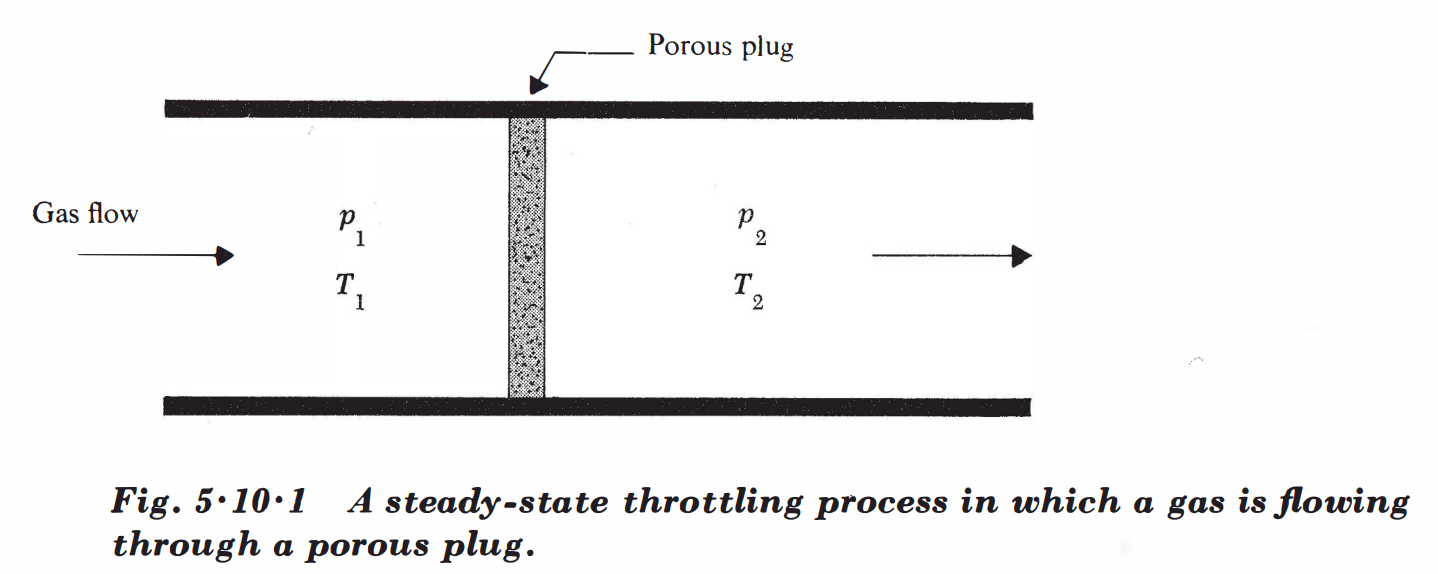
\includegraphics[scale=0.39]{plug.png}
\end{center}

A constant pressure difference is maintained with $p_1>p_2$. The question that we are interested in is that, if $T_1$ is temperature of gas on the LHS, what is the temperature of the RHS. Consider a mass $M$ of the gas on the LHS with volume $V_1$, the gas is being pushed by pressure $p_1$, hence work is done on the gas of mass $M$ on the LHS, by an amount of $p_1 V_1$. When the gas of mass $M$ is pushed to the RHS and now have volume $V_2$, then the gas of mass $M$ does work to other gas in pushing out the gas on the RHS, and the work done by the gas of mass $M$ is given by $p_2V_2$. Energy difference, that is, the energy increases as the gas is pushed through, is given by:
\begin{align*}
E_2 - E_1 = p_1 V_1 - p_2 V_2
\end{align*}
because the pipe is thermally insulated, energy only involves work, so rearranging we get:
\begin{align*}
E_2 + p_2 V_2 = E_1 + p_1 V_1
\end{align*}
\begin{center}
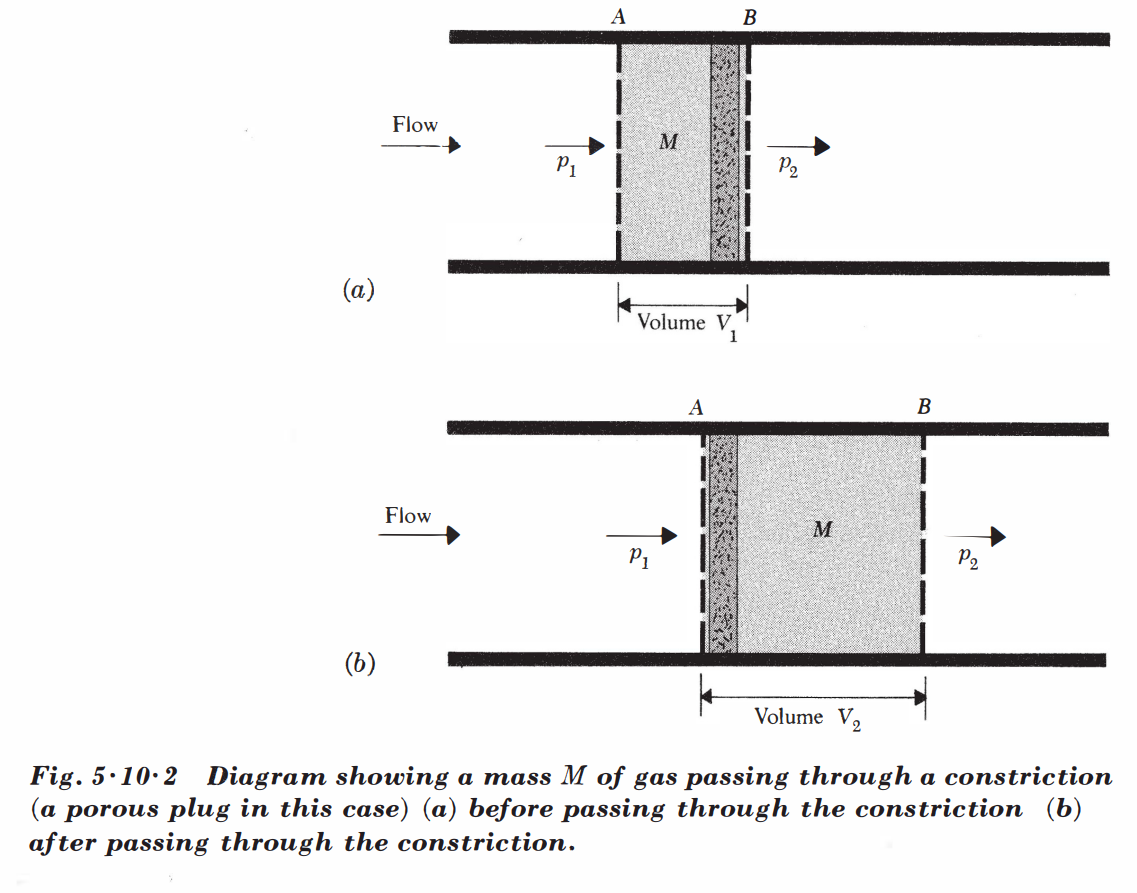
\includegraphics[scale=0.39]{plugAndM.png}
\end{center}

Hence the enthalpy is a constant in the Joule Thompson Process. That is, we write $H(T_1,p_1) = H(T_2, p_2)$. Now we will find the change in temperature of the gas of mass $M$. Now we can write $T(p,H)$ with the following:
\begin{align*}
dT = \lr{\frac{\pd T}{\pd p}}_H \, dp
\end{align*}
here $\lr{\frac{\pd T}{\pd p}}_H$ determines the change in temperature called Joule Thomson coefficient, denoted as:
\begin{align*}
\mu \coloneqq \lr{\frac{\pd T}{\pd p}}_H
\end{align*} 
Here we can write the following:
\begin{align*}
\lr{\frac{\pd T}{\pd p}}_H = -\frac{\lr{\frac{\pd H}{\pd p}}_T}{\lr{\frac{\pd H}{\pd T}}_p} 
= - \frac{T\lr{\frac{\pd S}{\pd p}}_T+V}{T \lr{\frac{\pd S}{\pd T}}_p} &= -\frac{-T\lr{\frac{\pd V}{\pd T}}_p + V}{T\lr{\frac{\pd S}{\pd T}}_p}\\
&= \frac{T\lr{\frac{\pd V}{\pd T}}_p - V}{C_p} \\
&= \frac{TV\alpha - V}{C_p} \\
&= \frac{V}{C_p}(T\alpha-1)
\end{align*}
For an ideal gas, we have $\mu = 0$ because $\alpha = \frac{1}{T}$.\\

For non-ideal gas, let us first analyze dependence of $T$ on $p$ at fixed $H$ for some real gasses Nitrogen (as given as example on Reif).
Here $H$ is a function of $T$ and $p$, when $H$ is fixed, we can expresses $T$ in terms of $p$, that is, $T$ as a function of $p$, and for different values of $H$, these relations between $T$ and $p$ form curves. That is, as the initial $T_1$ and $p_1$ are being specified on one curve, of fixed value $H$, the final temperature and pressure lie on the same curve as the initial ones. 
\begin{center}
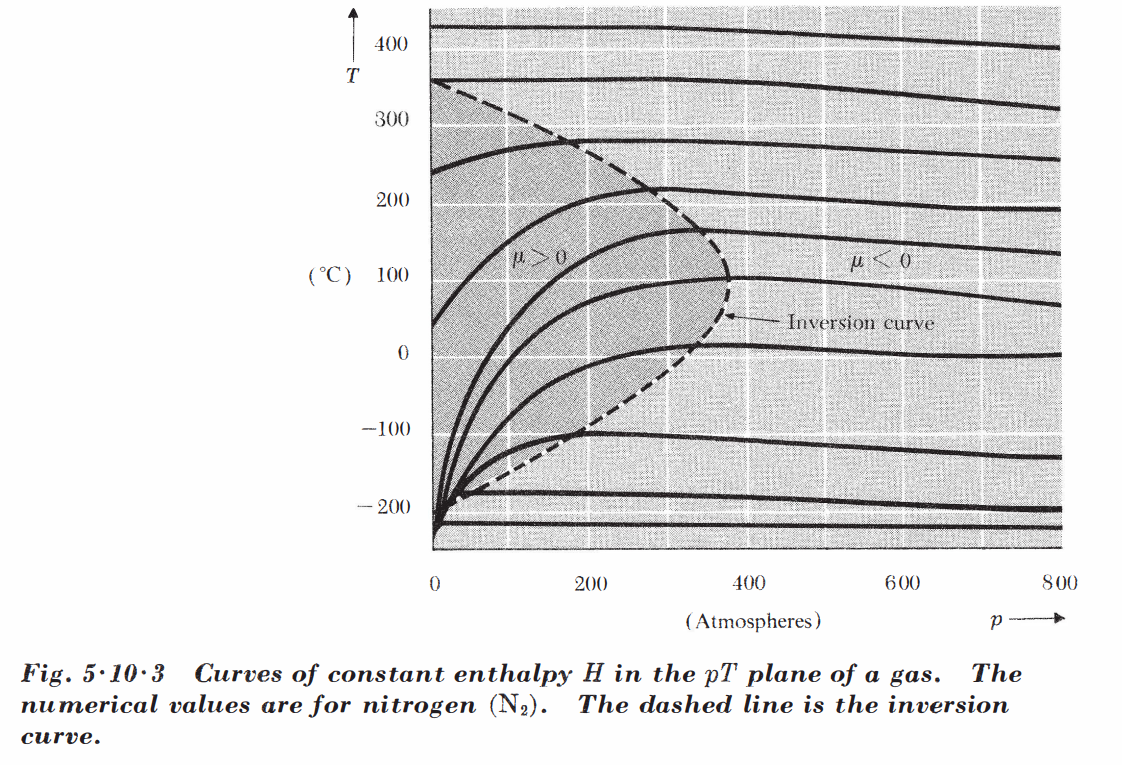
\includegraphics[scale=0.5]{N2JoulesThomson.png}
\end{center}
Note that $\mu$ by definition defines the slope of the curves. Then we know that $\mu = 0$ locates the maxima of the curves. The locas of the maxima is called the inversion curve. That is, the inversion curve passes through the point at $\mu = 0$ for all the level curves of fixed $H$. Note that $\mu>0$, and by construction we have $dp<0$ across the constriction, so for $\mu >0$, we have $dT<0$, and for $\mu<0$, we have $dT >0$.  That is, for values of $T,p$ inside the inversion curve, gas is cooled when pushed through the constriction. For values of $T,p$ outside the inversion curve, gas is heated when pushed through the constriction.\\

Here we want to investigate quantitative features using equation of state of a non-ideal gas.
For virial expansion, here we have:
$$\frac{p}{kT} = \frac{N}{V}\left(1+ B_2(T)N+\cdots \right)$$
where $B_2(T)$ is called the second virial coefficient, its behavior can be obtained from molecular consideration. \\

Here we can write:
\begin{align*}
\frac{p}{kT} \approx \frac{N}{V\left(1- B_2(T) \frac{N}{V}\right)} = \frac{N}{V - NB_2(T)} \qquad \Rightarrow \qquad V =\frac{NkT}{p} + NB_2(T)
\end{align*} 
where the first term comes from ideal gas, and the second term $NB_2(T)$ is the effect of interaction between particles. Quantum mechanics theory tells us that for long distance, the interaction forces are attractive. Consider now for small $T$ and large distance, that is, the kinetic energy of molecule is small, and interaction forces are mostly attractive. This setting tends to make interaction smaller, so $B_2(T)$ is negative for small $T$ and large distance. For large temperature and small distance, the kinetic energy of molecules is large and short range repulsion between molecules is dominant, so $B_2(T)$ is positive for large $T$ and small distance. \\

Here we can write:
\begin{align*}
V= \frac{NkT}{p}+NB_2(T) \qquad \Rightarrow \qquad \mu = \frac{1}{C_p}\left( T\lr{\frac{\pd V}{\pd T}}_p - V\right) = \frac{N}{C_p}\lr{T \frac{dB_2(T)}{dT} - B_2(T)}
\end{align*}
when $\mu = 0$, we have:
\begin{align*}
\frac{dB_2(T)}{dT} = \frac{B_2(T)}{T}
\end{align*}
For small $T$, we have $T\frac{dB_2}{dT} >0$, and $B_2<0$, so $\mu>0$. For large $T$, $B_2>0$, and at sufficiently large $T$, $\mu$ becomes negative. The inversion curve repeats the competing influence of the intermolecular force. \\

The Joule Thomson Process is not Quasi-stiatc.\\ 
Initial and final macrostates, and hence $H(T_1, p_1)$ and $H(T_2, p_2)$ are well defined.\\


For change in entropy, we have $S(p,H)$, and we can write:
\begin{align*}
dS = \lr{\frac{\pd S}{\pd p}}_H \, dp = - \frac{\lr{\frac{\pd H}{\pd p}}_S}{\lr{\frac{\pd H}{\pd S}}_p } \, dp = -\frac{V}{T}\, dp
\end{align*}
so we have $T\, dS = -V\, dp \neq 0$, but for the thermally insulated process, $\dbar Q = 0$, hence we have $T\, dS \neq \dbar Q$ because the process is not Quasi-static.\\

\newpage
\section[Heat Engine]{\color{red}Heat Engine\color{black}}
The most general heat engine is an isolated system consisting of heat sources, work sources, working subsystems. Note that the system is isolated, so no energy transferred into or out of the system. \\

Reversible heat sources are heat reservoirs at constant $V$ and $T$, which cannot do work, and all processes are Quasi-static. Here we can write the following since there is no work done:
\begin{align*}
\Delta S = \frac{Q}{T} = \frac{\Delta E}{T}
\end{align*}
Reversible work sources have fixed $p$ and fixed $S$, which cannot absorb heat, and all processes are Quasi-static. Here we can write the following:
\begin{align*}
W = -\Delta E \qquad\qquad\qquad\qquad\qquad \Delta S= 0
\end{align*}
Working subsystems can exchange both heat and work between the heat source and the work source, example includes gas in a thermally conducting cylinder with moving piston. \\

When constraints are removed, the whole system will adjusts to maximize entropy. \\

For irreversible processes, we have $\Delta S >0$. Consider the following example: suppose we have two heat sources, one with temperature $T_H$ and the other one with temperature $T_C$, with $T_H>T_C$, heat $Q$ is flowing from the source with $T_H$ to the one with $T_C$. Then we can write:
\begin{align*}
\frac{Q}{T_C} > \frac{Q}{T_H}
\end{align*}
If any step is not Quasi-static, then process is irreversible. \\

For reversible process, we have $\Delta S = 0$.\\

Now we want to investigate in what condition work is done a maximum. Consider in an heat engine we have heat source $T_C$, a work source, and a working subsystem changing state from $A$ to $B$. In state $A$, energy is $E_A$ and entropy is $S_A$, in state $B$, energy is $E_B$ and entropy is $S_B$.\\ 

Going from state $A$ to state $B$: \\
For the total system, entropy increases by $\Delta S \geq 0$, and energy increases by $0$ because the system is isolated. For the subsystem, change in entropy is $S_B - S_A$, and change in energy is $E_B-E_A$. For the heat source, change in entropy is given by $\Delta S - (S_B - S_A)$, and the energy increase is give by $T_C(\Delta S-(S_B - S_A)) = T_C \Delta S - T_C(S_B-S_A)$. For the work source, increase in entropy is $0$, and the increase in energy is given by $E_A - E_B - T_C\Delta S + T_CS_B -T_CS_A = (E_A - T_CS_A) - (E_B - T_CS_B)-T_C\Delta S$. \\

Here we observe that, since $\Delta S \geq 0$, energy delivered to work source is at maximum when $\Delta S = 0$, in which case the process is reversible. Here $E - T_CS$ represents the potentials for doing work, if a heat source is available to absorb heat at temperature $T_C$.\\

For subsystem undergoing a cyclic process, the system return to the initial state for each cycle, so no change in $S$ for subsystem, Maximum work requires reversible process for whole system such that $\Delta S = 0$. If the working subsystem absorbs heat $Q_H$ from heat source $T_H$, dumps heat to the heat source $Q_C$, and perform work $W$ to the work source, then we have we have:
\begin{align*}
\Delta S = 0 \qquad \Rightarrow \qquad \frac{Q_C}{T_C} - \frac{Q_H}{T_H} = 0 \qquad \Rightarrow \qquad \frac{Q_C}{T_C} = \frac{Q_H}{T_H}
\end{align*}
with the following:
\begin{align*}
Q_C = \frac{Q_HT_C}{T_H}\qquad \Rightarrow \qquad W = Q_H - Q_C= Q_H \left(1- \frac{T_C}{T_H}\right)
\end{align*}

The efficiency of such system is then given by:
\begin{align*}
\eta = \frac{W}{Q_H} = 1-\frac{T_C}{T_H}
\end{align*}
note that the efficiency is the ratio of the work done to the heat provided by heat source $T_H$. 

\newpage
\subsection{Carnot Engine Cycle}
The process of Carnot Cycle:
\begin{enumerate}[topsep=3pt,itemsep=-1ex,partopsep=1ex,parsep=1ex]
\item Open the valve $C$, and compress the gas isothermally. Some heat will go out, denoted as $Q_C$.
\item Close the valve $C$, and compress the gas adiabatically. 
\item Open the valve $H$, and expand the gas isothermally. Some heat is absorbed, denoted as $Q_H$.
\item Close the valve $H$, and expand the gas adiabatically.
\end{enumerate}

\hfill\break
In process (1), heat goes out from the system, hence $Q_C<0$, and hence the change in entropy is negative. Also, the gas is compressed, so work done is negative.\\

In process (2), no heat transfer, so change in heat is zero, and hence the change in entropy is zero. Also, the gas is compressed, so work done is negative.\\

In process (3), heat goes into the system, hence $Q_C>0$, and hence the change in entropy is positive. Also, the gas is expanded, so work done is positive.\\

In process (4), no heat transfer, so change in heat is zero, and hence the change in entropy is zero. Also, the gas is expanded, so work done is positive.\\

The net heat absorbed by the gas is then given by:
\begin{align*}
Q_H - Q_C
\end{align*}

After each cycle, the gas, the subsystem of the whole system, is back to the original state, but the whole system is not. To restore the system back, one can reverses the entire process: (4) close valve $C$ and compress adiabatically, (3) open valve $H$ and compress isothermally, (2) close valve $H$ and expand adiabatically, and (1) open valve $C$ and expand isothermally. Each of these processes is Quasi-static.\\

\newpage
\chapter{Canonical Ensemble}
\section[The Partition Function]{\color{red} The Partition Function\color{black}}
Canonical ensemble describes a system in contact with a heat bath at temperature $T$.\\

An isolated system in equilibrium with energy $E$ is represented by a microcanonical ensemble. Each state $r$ in such ensemble has equal probability $p_r$, written as the following:
\begin{align*}
p_r = \begin{cases}
\text{constant} & E\leq E_r \leq E+\delta E\\
0 & \text{otherwise}
\end{cases}
\end{align*}

\begin{center}
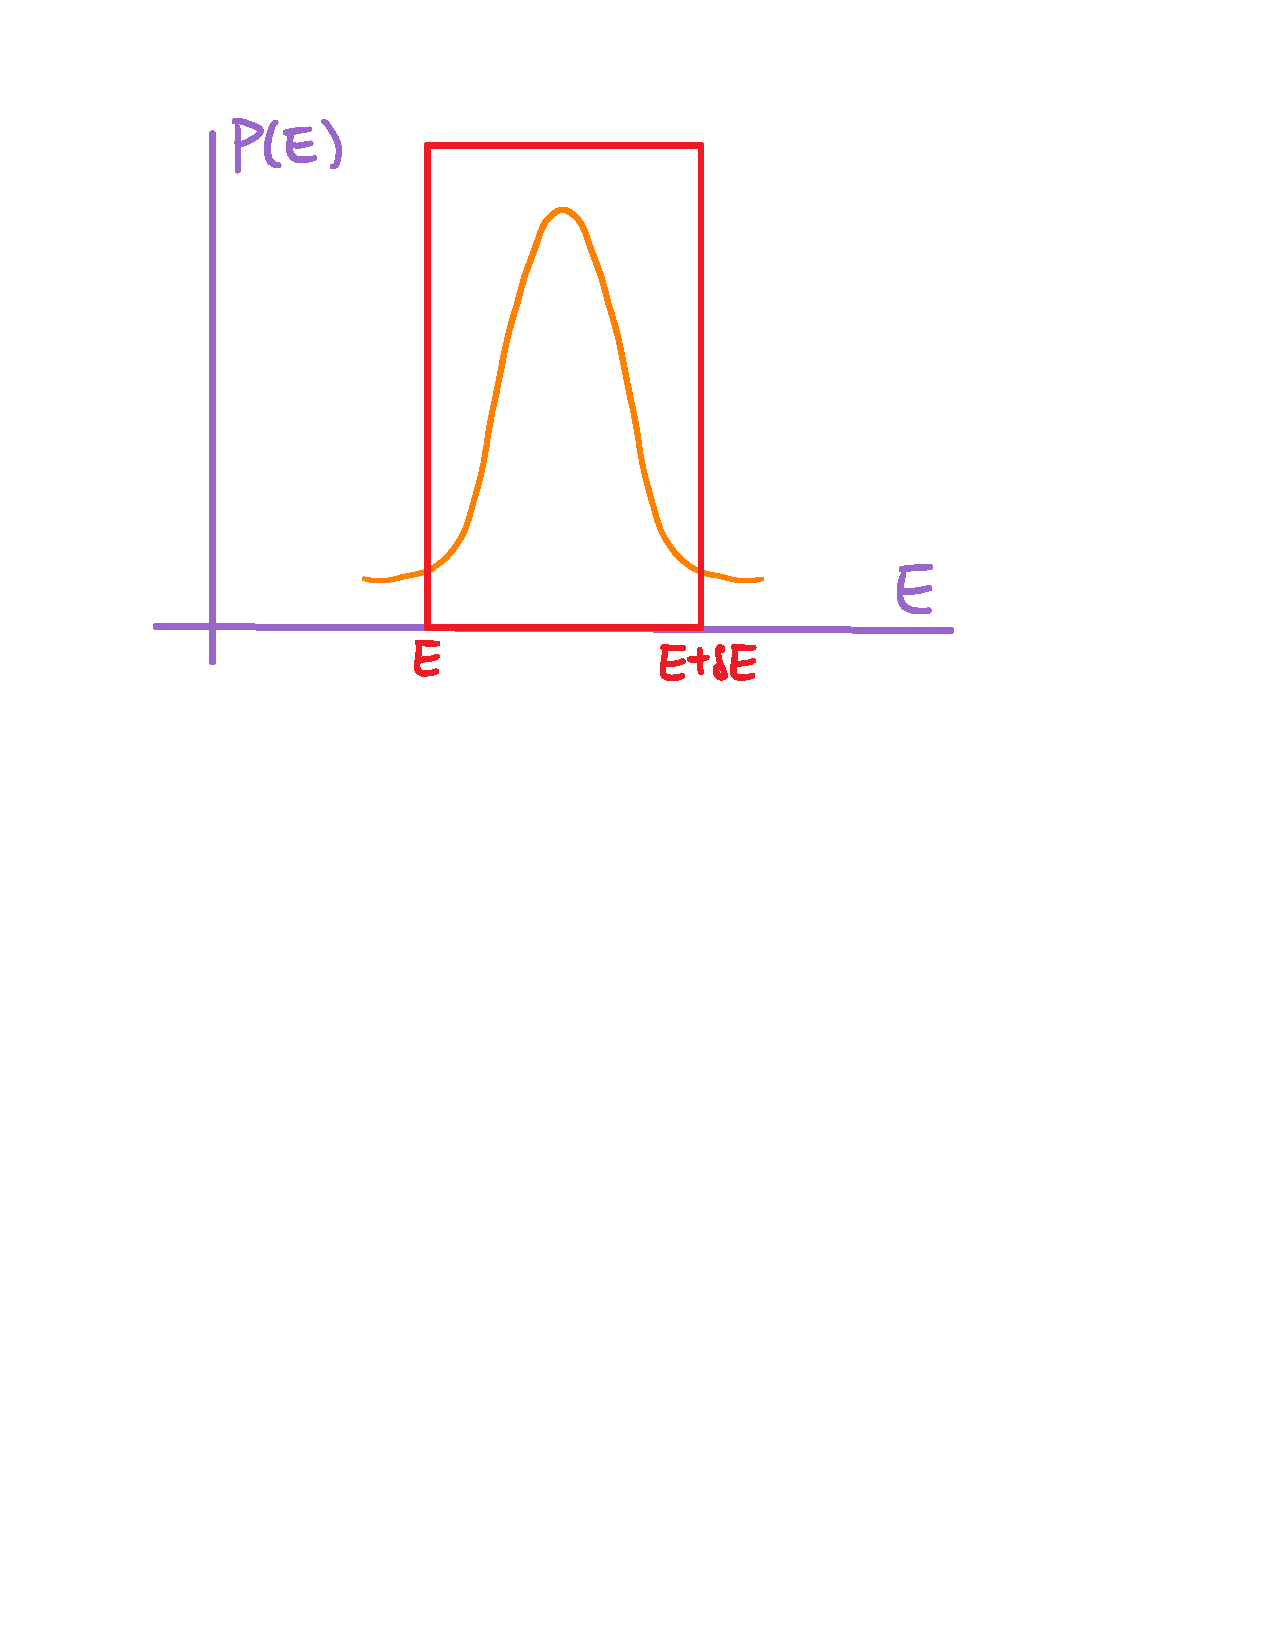
\includegraphics[scale=0.5]{peak.pdf}
\end{center}

This has some unpleasant features once interaction between subsystems is introduced:
\begin{enumerate}[topsep=3pt,itemsep=-1ex,partopsep=1ex,parsep=1ex]
\item Hard to count the number of states in this system
\item It is unrealistic to assume such sharp boundary for the allowed energy
\item When subsystems interact thermally, the probability distribution changes, even when the whole system is isolated. 
\end{enumerate}
Hence a microcanonical ensemble is not a very realistic description. \\

\hfill\break
A canonical ensemble represents a system $A$ in thermal equilibrium with a heat reservoir $A'$ at temperature $T$. We want to find the probability for a state $r$ in $A$ with energy $E_r$. Note that $A$ along with $A'$ is assumed to be isolated, denote the energy of $A'$ as $E'$, here we have $E_r + E' = E_0$, with $E_0$ being fixed. Also note that we can write:
\begin{align*}
p_r \propto \Omega \cdot \Omega'(E_0 - E_r) \propto \Omega'(E_0 - E_r)
\end{align*}
where $\Omega$ is the state accessible to $A$, since we are interested in state $r$ particularly, then $\Omega = 1$. 
Assuming that $E_r<< E_0$, then we can write the Taylor Expansion of $\Omega'(E_0-E_r)$ about $E_r = 0$:
\begin{align*}
\ln\left(\Omega'(E_0 - E_r)\right)  &= \ln(\Omega'(E_0))+ \lr{\frac{\partial (\ln(\Omega'))}{\partial E_r}}_{E_r = 0}\, E_r + \cdots  \\
&= \ln(\Omega'(E_0))- \lr{\frac{\partial (\ln(\Omega'))}{\partial E'}}_{E_r = 0}\, E_r + \cdots 
\end{align*}
Note that $p_r = \text{constnat } \cdot \Omega'(E_0 - E_r)$, hence we have:
\begin{align*}
 \ln (p_r) = \text{constant} + \ln(\Omega'(E_0) )- \lr{\frac{\partial (\ln(\Omega'))}{\partial E'}}_{E_r = 0} E_r + \cdots 
\end{align*}
Since we have $\beta ' (E') = \beta(E)$ at equilibrium, then with $c = \text{constant}+\ln(\Omega'(E_0))$, we have:
\begin{align*}
\ln(p_r) \approx c - \beta E_r\qquad\Rightarrow \qquad p_r = ce^{-\beta E_r} = ce^{-\frac{E_r}{kT}}
\end{align*}
Normalize the distribution, we require $\sum_r p_r = 1$, hence we have:
\begin{align*}
 c \sum_r e^{-\beta E_r} = 1 \qquad \Rightarrow \qquad c = \frac{1}{\sum_r e^{-\beta E_r}} \qquad \Rightarrow \qquad p_r = \frac{e^{-\beta E_r}}{\sum_r e^{-\beta E_r}}\tag{PR}
\end{align*}
The quantity $z = \sum_r e^{-\beta E_r}$ is called the partition function, we will see that knowing $z$ gives us complete information about the system. There is therefore a relationship between partition function and thermodynamic potentials. \\

Note here the ground state with the least energy is the most probable state by equation (PR). \\

The probability that the system $A$ has an energy $E$, denoted as $p(E)$, is given by:
\begin{align*}
p(E) \propto p_r(E) \cdot \Omega(E)
\end{align*}
here $\Omega(E)$ is the number of states with energy $E$. \\

\begin{center}
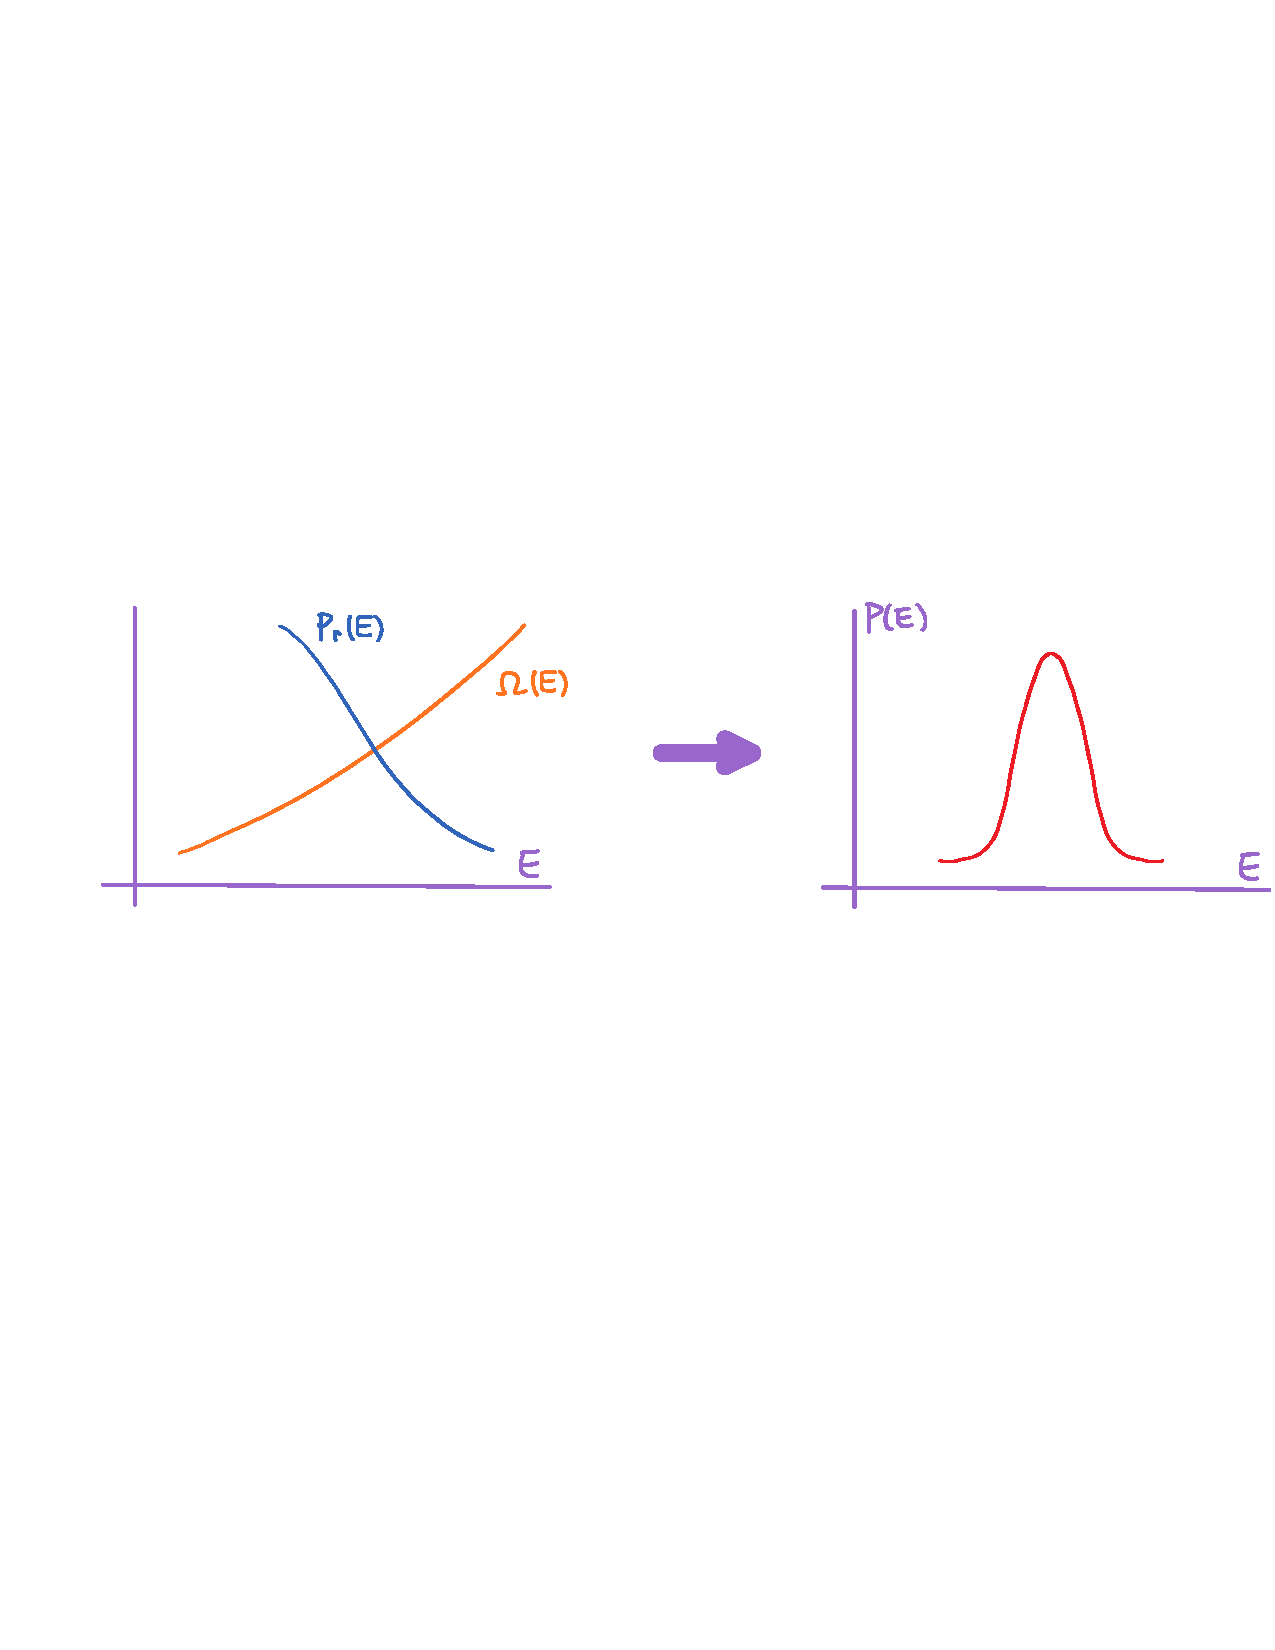
\includegraphics[scale=0.65]{canEnsemble.pdf}
\end{center}

For a system with many degrees of freedom $f$, we have $\Omega(E) \propto E^f$, $p(E) = p_r(E) \Omega(E) \propto e^{-\beta E} E^f$, and hence we can write the following:
\begin{align*}
 \ln(p(E)) = -\beta E + f\ln(E) + \text{constant}
\end{align*}
Hence the maximum of the probability distribution is given by:
\begin{align*}
\frac{\partial \ln(p(E))}{\partial E} = 0 \qquad \Rightarrow \qquad -\beta + f/E = 0
\end{align*}
So the most likely energy is given by: 
$$\widetilde{E} = \frac{f}{\beta} = \frac{f}{kT}$$\\

\subsection*{Another Approach to the Derivation of Canonical Ensemble}
The criteria for choosing an ensemble is maximizing missing information subject to constraints. That is, we are maximizing $S/k = -\sum_r p_r \ln(p_r)$, under constraint $\sum_r p_r = 1$, and $\bar{E} = \sum_r p_r E_r$ being fixed. In other words, we can write, with $\alpha$ and $\beta$ being constants:
\begin{align*}
\frac{\partial}{\partial p_i}\left(\frac{S}{k} - \alpha\sum_r p_r - \beta \sum_r  p_r E_r \right) = 0
\end{align*}
That is, we have:
\begin{align*}
-\ln(p_i) - 1 - \alpha - \beta E_i = 0 \qquad \Rightarrow \qquad p_i = (e^{-1 - \alpha})e^{-\beta E_i}
\end{align*}
pick $\alpha$ and $\beta$ such that $\sum_i p_i = 1$ and $\sum_r p_i E_i = \bar{ E}$. \\

\newpage
\subsection{Connection of the Partition Function with Thermodynamics}
Here we can write:
\begin{align*}
\bar{E} = \sum_r p_r E_r = \frac{\sum_r E_r e^{-\beta E_r}}{z}
\end{align*}
where $z = \sum_r e^{-\beta E_r}$. Note that we have:
\begin{align*}
\frac{\partial z}{\partial \beta} = -\sum_r E_r e^{-\beta E_r}
\end{align*}
Combining we get:
\begin{align*}
\bar{E} = -\frac{1}{z}\frac{\partial z}{\partial  \beta} = -\frac{\partial }{\partial \beta}\ln(z)
\end{align*}
The generalized force can be written as:
\begin{align*}
\bar{X} = -\frac{\partial \bar{E}}{\partial x} = -\sum_r p_r \frac{\partial E_r}{\partial x} = \frac{-\sum_r e^{-\beta E_r} \frac{\partial E_r}{\partial x}}{z}
\end{align*}
hence we have:
\begin{align*}
\frac{\partial z}{\partial x} = \sum_r -\beta \frac{\partial E_r}{\partial x}e^{-\beta E_r} \qquad \Rightarrow \qquad \bar{X} = \frac{1}{\beta}\frac{\partial \ln(z)}{\partial x}
\end{align*}
Note that $z$ is a function of $\beta$ and $x$, hence we have:
\begin{align*}
d(\ln(z)) = \left.\frac{\partial (\ln(z))}{\partial \beta}\right|_{x}\, d\beta + \left.\frac{\partial (\ln(z))}{\partial x}\right|_{\beta}\, dx = -\bar{E}\, d\beta + \beta \bar{X}\, dx = -\bar{E}\, d\beta + \beta \dbar W 
\end{align*}

For Quasi-static process, we get:
\begin{align*}
dS = \frac{\dbar Q}{T} = k\beta \, \dbar Q &= k(\beta \dbar W+ \beta d\bar{E})= k\left(d\ln(z) + \bar{E}\, d\beta + \beta d\bar{E}\right)= d(k\ln(z) + k\beta \bar{E})
\end{align*}
Here we see that we can identify $S$ up to a constant:
\begin{align*}
S = k\left( \ln(z) + \beta \bar{E}\right) +C
\end{align*}
In fact, this relation is true in general, not just for Quasi-static process, because we have:
\begin{align*}
S = -k\sum_r p_r \ln(p_r) &= -k\sum_r p_r \ln \left(\frac{e^{-\beta E_r}}{z} \right) \\
&= -k \sum_r p_r \left( \ln(e^{-\beta E_r}) - \ln(z)\right) \\
&= -k \sum_r p_r\left( -\beta E_r - \ln(z) \right) \\
&= k\sum_r\left( p_r \beta E_r + p_r \ln(z) \right) \\
&= k\beta \bar{E} + k \ln(z)
\end{align*}

Now we can write:
\begin{align*}
k\ln(z) &= S- k\beta \bar{E} \qquad\Rightarrow\qquad  kT\ln(z) = TS - (kT)\beta \bar{E}= TS -\bar{E}=-F 
\end{align*}
where $F$ is the Helmholtz free energy, hence we obtain the following:
\begin{align*}
F(T,V) = -kT\ln(z)
\end{align*} 
Note that, thermodynamically, everything can be derived from $F(T,V)$, and in statistical mechanics, everything can be derived from the partition function. \\
\newpage

\subsection{Partition Function for a Weakly Interacting System}
In discussion above, $z$ was introduced by considering a system in contact with a heat bath, the same argument can be applied if the system $A$ is a small identifiable part of the whole system $A^0$, with $A'$ being the heat bath. Here $A,A'$ constitutes subsystems of $A^0$.\\

Now consider two weakly interacting systems in thermal contact.\\
${}$\quad System A: states $r$, energies $E_R$, temperature defined by $\beta$\\
${}$\quad System B: states $s$, energies $E_s$, temperature defined by $\beta'$\\
Question: When the total system can be represented by a canonical ensemble.\\
 
For system $A$, we can write the following:
\begin{align*}
p_r = \frac{e^{\beta E_r}}{z_A} \qquad \qquad \qquad z_A = \sum_r e^{-\beta E_r}
\end{align*}
and for system $B$, we can write the following:
\begin{align*}
p_s = \frac{e^{\beta' E_s}}{z_B} \qquad \qquad \qquad z_B = \sum_s e^{-\beta' E_s}
\end{align*}
when the two are in contact with each other, we can write:
\begin{align*}
p_{rs} = p_r \cdot p_s = \frac{e^{-(\beta E_r + \beta' E_s)}}{z_A z_B}
\end{align*}
This distribution is canonical only if $\beta = \beta'$.\\ 

Now consider a system composed of $N$ identifiable parts.
\begin{center}
Part 1 has states $r_1$, energies $E^{(1)}_{r_1}$\\
Part 2 has states $r_2$, energies $E^{(1)}_{r_2}$
$$\vdots$$
Part $N$ has states $r_N$, energies $E^{(N)}_{r_N}$
\end{center}

For the entire system, we can write:
\begin{align*}
E_{r_1,r_2,\cdots, r_n} = E_{r_1}^{(1)}+E_{r_2}^{(2)}+\cdots + E_{r_N}^{(N)} 
\end{align*}
Here we assumed that the parts are weakly interacting, then we can write:
\begin{align*}
z &= \sum_{r_1,r_2,\cdots, r_n} e^{-\beta E_{r_1,r_2,\cdots, r_n}}\\
&= \sum_{r_1,r_2,\cdots, r_n} e^{-\beta \left( E_{r_1}^{(1)}+E_{r_2}^{(2)}+\cdots + E_{r_N}^{(N)}  \right)}\\
&= \left( \sum_{r_1} e^{-\beta E_{r_1}^{(1)}}\right)\left( \sum_{r_2} e^{-\beta E_{r_2}^{(2)}}\right)\cdots \left( \sum_{r_N} e^{-\beta E_{r_N}^{(N)}}\right)\\
&= z^{(1)} z^{(2)}\cdots z^{(N)}
\end{align*}
so we have 
$$\ln(z) = \sum_{i=1}^N \ln (z^{(i)}) + \text{quantiles such as }F, E, S, \bar{X}$$
\hfill\break
To find partition function of many weakly interacting portions, which are considered to be identifiable, of a system. First we need to calculate $\ln(\rho)$ for each portion of partition, where $\rho$ is the partition function of that portion, then add up $\ln(\rho)$ to find $\ln(z)$ for the whole system. Note that we can differentiate $z$ to get thermodynamics quantities of interest. \\

\newpage

\example Spin half atoms in a magnetic field.\\
There are two types of atoms in space, one has magnetic moment $\mu$ and the other one has magnetic moment $\mu'$. There are $N$ of them have magnetic moment $\mu$ and $N'$ of them have magnetic moment $\mu'$\\

Each atom plays the role of an identifiable part, and they only have two possible energy levels, $\mu H$ or $-\mu H$ for atoms with magnetic moment $\mu$, and $\mu' H$ or $-\mu' H$ for atoms with magnetic moment $\mu'$.\\

Partition function for each atom with $\mu$ is then given by the following:
\begin{align*}
\rho = e^{-\beta \mu H} + e^{\beta \mu H} = 2\cosh (\beta \mu H)
\end{align*}
Partition function for each atom with $\mu'$ is given by the following:
\begin{align*}
\rho' = e^{-\beta \mu' H} + e^{\beta \mu' H} = 2\cosh (\beta \mu' H)
\end{align*}
Hence the partition function for the whole system $z$ satisfies:
\begin{align*}
\ln(z) = N \ln(\rho) + N' \ln (\rho') = N \ln(2\cosh(\beta \mu H)) + N' \ln( 2\cosh(\beta \mu' H))
\end{align*}


\newpage
\section[The Gibbs Paradox]{\color{red}The Gibbs Paradox\color{black}}
Consider a classical monoatomic gas, the Hamiltonian of such gas is given by the following:
\begin{align*}
\mathcal{H} = \sum_{i=1}^N \frac{p_i^2}{2m}+\text{negligible potential energy }U(r_1,r_2,\cdots, r_n) 
\end{align*}
where $p_i$ is the momentum of each of the gas molecule, and there are $N$ molecules in the system.\\

Each molecule can be considered as an identifiable portion, the rest of the gas serve as a heat bath for the molecule. Here we will try to find the partition function for each molecule. We can write the following to denote the partition function for each of the molecules:
\begin{align*}
\rho = \sum_{\text{states } r} e^{-\beta E_r}
\end{align*}
For classical weakly interacting gas, we have $E_r$ is a function of momentum of the molecules, and the momentum $p$ is continuous. Divide the entire phase space into cells of size $h_0$, then the following is the number of states in a cell of volume $h_0^3$:
\begin{align*}
\frac{dx\, dp_x}{h_0} \frac{dy\, dp_y}{h_0} \frac{dz dp_z}{h_0} \tag{*}
\end{align*}
Summing all the states is equivalent to integrating equation (*) over the phase space.\\ 
Hence we have:
\begin{align*}
\rho  &=  \frac{1}{h_0^3}\int_V dx\, dy\, dz \int_{-\infty}^{\infty} dp_x \, \int_{-\infty}^{\infty} dp_y \, \int_{-\infty}^{\infty} dp_z \ e^{-\frac{\beta}{2m}{(p_x^2+p_y^2+p_z^2)}} \\
&=  \frac{V}{h_0^3}\int_{-\infty}^{\infty}e^{-\frac{\beta}{2m}{p_x^2}} dp_x \, \int_{-\infty}^{\infty} e^{-\frac{\beta}{2m}{p_y^2}}dp_y \, \int_{-\infty}^{\infty} e^{-\frac{\beta}{2m}{p_z^2}} dp_z \  \\
&= \frac{V}{h_0^3}\left(\sqrt{\frac{2m\pi}{\beta}}\sqrt{\frac{2m\pi}{\beta}}\sqrt{\frac{2m\pi}{\beta}}\right)\\
&= \frac{V}{h_0^3}\left( \frac{2\pi}{\beta}\right)^{3/2}
\end{align*}
For $N$ molecules in the gas, each identifiable, we have:
\begin{align*}
\ln(z) = N \ln (\rho) = N \left( \ln(V) - \frac{3}{2}\ln(\beta) + \frac{3}{2}\ln\left( \frac{2m \pi}{h_0^2}\right)\right)
\end{align*}
Here we see that we have:
\begin{align*}
E = -\frac{\partial \ln(z)}{\partial \beta} = -N\left(- \frac{3}{2\beta}\right) = \frac{3}{2}\frac{N}{\beta} = \frac{3}{2}NkT
\end{align*}
and we have:
\begin{align*}
\bar{p} = \frac{1}{\beta}\frac{\partial \ln(z)}{\partial V} = \frac{1}{\beta} \frac{N}{V} = \frac{NkT}{V}
\end{align*}
For the entropy, we can write:
\begin{align*}
S 
&= k\left( \ln(z) +\beta \bar{E}\right) \\
&= Nk\left( \ln(V) + \frac{3}{2}\ln\left(kT\right) + \frac{3}{2}\ln\left(\frac{2m\pi}{h_0^2}\right)\right) + \frac{3}{2}Nk\\
&= Nk\left(\ln(V) + \frac{3}{2}\ln(T)+ \sigma\right) \tag{PSE}
\end{align*}
where we have:
\begin{align*}
\sigma = \frac{3}{2}\left( \ln\left( \frac{2mk\pi}{h_0^2}\right) + 1\right)
\end{align*}
Here we see that $\sigma$ is a constant. In fact, this expression for entropy given by equation (PSE) is not correct. Problems with this expression for entropy where we have assumed that gas molecules are identifiable has to do with the fact that in quantum mechanics particles are considered identical.\\

\hfill\break
\hfill\break
Now consider a box of gas split into two halves by a partition. Each with parameters $N,V,S$. That is, we have same gas in both compartments. For each half of the box, and results from discussion above, the entropy for the gas in this half of the box is given by the following:
\begin{align*}
S = Nk\left(\ln(V) + \frac{3}{2}\ln(T) + \sigma\right)
\end{align*}

Now we remove the partition, since the gas in both compartments are the same, nothing should happen while removing the partition, hence we must have $\Delta S = 0$ because we can restore the original configuration by putting the partition back. However, after the partition is removed, we have $2N$ molecules, $2V$ volumes, and entropy given by:
\begin{align*}
S_{\text{new}} = 2Nk\left( \ln(2V)+ \frac{3}{2}\ln(T) + \sigma\right)
\end{align*} 
Note here the entropy, if nothing happened, should be:
\begin{align*}
2S = 2Nk\left( \ln(V) + \frac{3}{2}\ln(T) + \sigma\right)
\end{align*}
and here we have: 
\begin{align*}
S_{\text{new}} - 2S = 2Nk\ln(2) \neq 0
\end{align*}
If the gases were different $\Delta S \neq 0$ is fine because the gas would mix, but for the same kind of gas on both sides, $2S$ must be equal to $S_{\text{new}}$ such that $\Delta S = 0$. The entropy we have obtained is not additive. This problem is known as the Gibbs Paradox.\\

\begin{center}
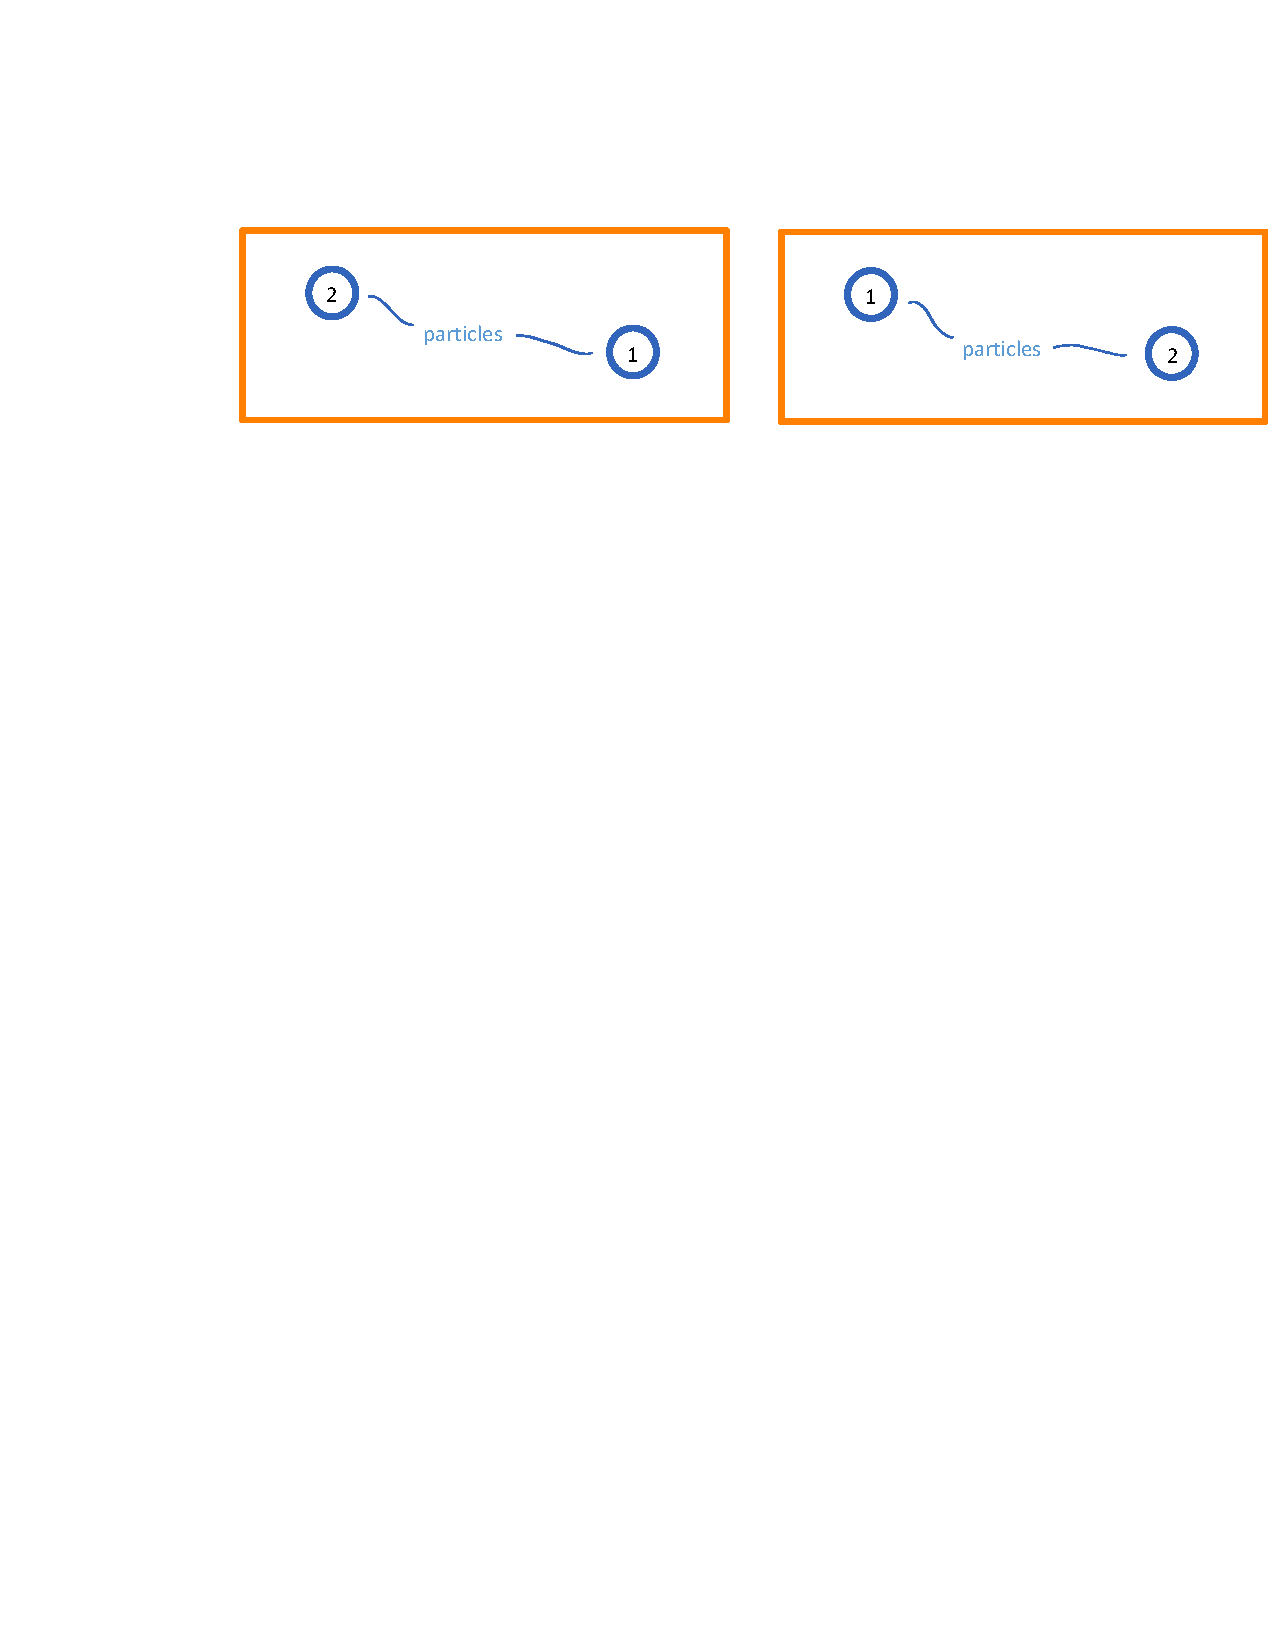
\includegraphics[scale=0.69]{gibbsPar.pdf}
\end{center}

These two situations were counted differently as identifiable portions in our derivation. While in quantum mechanics, they describe the same state using the same wave function because of the identity of molecules 1 and 2, as they are exactly identical molecules. Hence we have overcounted the number of states. The two states above should be counted as a single state, not two separate states. For $N$ molecules, we have overcounted $N!$ states because there are $N!$ permutations which give the same state, so ad hoc remedy is to divide number of state by $N!$. \\

Denote the new partition function, after the correction, as $z$, and denote the old partition function, before the correction, as $z_{old}$, here we require:
\begin{align*}
z_{new} = \frac{z_{old}}{N!}
\end{align*}
and hence we can write:
\begin{align*}
\ln(z) = \ln(z_{old}) - \ln(N!)
\end{align*}
note that $\ln(N!) \approx N \ln(N) - N$ for large $N$, so we can write:
\begin{align*}
\ln(z) &= N\left( \ln(V) + \frac{3}{2}\ln(T) + \sigma - \ln(N) + 1\right) \\
&= N \left( \ln\left(\frac{V}{N}\right) +\frac{3}{2}\ln(T) + \sigma_0\right)
\end{align*}
where we define $\sigma_0 = \sigma + 1$, hence we obtain:
\begin{align*}
S = k\left(\ln(z) + \beta \bar{E} \right) = Nk\left( \ln\left(\frac{V}{N}\right) + \frac{3}{2}\ln(T) + \sigma_0\right)
\end{align*}
with $\sigma_0$ being independent of $N,V,T$. Now we will check that the entropy is extensive variable. Consider two gasses of the same type but with different number of molecules in different volume, gas A has parameters $N,V,T$, and gas B has parameter $2N, 2V, T$, and the mixture of gas $A$ and gas $B$ has parameters given by $2N$, $2V$, $T$. Here we can write:
\begin{align*}
S_A = Nk\left( \ln\left(\frac{V}{N}\right) + \frac{3}{2}\ln(T) + \sigma_0\right) \qquad\qquad\qquad
S_B = 2Nk\left( \ln\left(\frac{2V}{2N}\right) + \frac{3}{2}\ln(T) + \sigma_0\right)
\end{align*}
\begin{align*}
S_{A+B} &= Nk\left( \ln\left(\frac{2V}{N}\right) + \frac{3}{2}\ln(T) + \sigma_0\right)+  Nk\left( \ln\left(\frac{2V}{N}\right) + \frac{3}{2}\ln(T) + \sigma_0\right)\\
&= 2Nk\left( \ln\left(\frac{2V}{N}\right) + \frac{3}{2}\ln(T) + \sigma_0\right)
\end{align*}
Here we see that $S_B = 2S_A$ which shows that entropy is extensive, and we have $S_{A+B} - S_B = 2Nk\ln(2) \neq 0$ because there is entropy of mixing. Now everything is consistent. \\
\newpage



\newpage
\section[Paramagnetism]{\color{red}Paramagnetism\color{black}}
$N_0$ atoms each with magnetic moment $\vec{\mu}$ are palced in a magnetic field $\vec{H}$. \\
For each atom, the energy is given by:
\begin{align*}
E = -\vec{\mu}\cdot \vec{H}
\end{align*}
where we have:
\begin{align*}
\vec{\mu} = g\mu_0 \vec{J} \qquad\qquad\qquad \mu_0 =\frac{e\hbar}{2m_e c}
\end{align*}
here $g$ is of order $1$, called the $g$-factor. Energy of each atom is given by:
\begin{align*}
E = -g \mu_0 J_z H
\end{align*}
according to quantum mechanics, allowed values of $J_z$ is given from $-J$ to $J$. \\
Then the Partition Function for each atom is given by the following:
\begin{align*}
\rho &= \sum_r e^{-\beta E_r} \\
&= \sum_{m=-J}^{J} e^{\beta \mu_0 gmH}\\
&= e^{-\beta \mu_0 gJH} \lr{1+ e^{\beta \mu_0 gH}+ e^{2\beta \mu_0 gH}+\cdots + e^{2\beta \mu_0 gJH}} \\
&= e^{-\beta g\mu_0 JH} \frac{1- e^{\beta \mu_0 gH (2J+1)}}{1-e^{\beta \mu_0 gH}}\\
&= \frac{\sinh\lr{J+\frac{1}{2}}\beta \mu_0 gH}{\sinh\lr{\frac{1}{2}\beta \mu_0 gH}}
\end{align*}
For partition function $z$ for $N_0$ atoms, we get:
\begin{align*}
\ln(z) = N_0 \ln(\rho) = N_0 \lr{\ln\lr{\sinh\lr{J+\frac{1}{2}} \beta \mu_0 gH} - \ln\lr{\sinh\lr{\frac{1}{2}\beta \mu_0 gH}} }
\end{align*}
Mean magnetic moment is given by:
\begin{align*}
\left< \mu_z\right> = M \qquad\qquad\qquad\qquad \mu_z = g\mu_0 m
\end{align*}
For each atom:
\begin{align*}
\left< \mu_z \right>_0 = \frac{\sum_{m=-J}^{J} g\mu_0 me^{\beta \mu_0 gmH}}{\sum_{m=-J}^{J}e^{\beta \mu_0 gmH}} = \frac{1}{\beta}\frac{\partial }{\partial H}\lr{\ln(\rho)}
\end{align*}
For $N_0$ atom, we get:
\begin{align*}
M = \frac{1}{\beta}\frac{\partial}{\partial H}\lr{\ln(z)} = N_0 \mu_0 g\lr{\lr{J+\frac{1}{2}}\coth\lr{\lr{J+\frac{1}{2}}\beta \mu_0 gH}-\frac{1}{2}\coth\lr{\frac{1}{2}\beta\mu_0 gH}}
\end{align*}
Now consider the high temperature limit, that is, we have $kT >> \mu_0 gH$, or $\beta << \mu_0 gH$, one can use the expansion of $\coth$ given by the following:
\begin{align*}
\coth(x)\approx \frac{1}{x}+ \frac{x}{3}+\cdots \qquad\text{for small }x
\end{align*}
and get a simplification for $M$:
\begin{align*}
M \approx \frac{N_0\mu_0 g}{3}J(J+1) \beta \mu_0 gH = \frac{N_0 \mu_0^2 g^2 J(J+1)}{3kT}\, H
\end{align*}
Define suseptibility $\chi$ by $M = \chi H$, we get:
\begin{align*}
\chi = \frac{N_0 \mu_0^2 g^2 J(J+1)}{3kT} \tag{Curie's Law}
\end{align*}
Curie's Law has been verified experimentally.
\newpage

\chapter{Equipartition}
\section[The Equipartition Theorem]{\color{red} The Equipartition Theorem\color{black}}
\begin{thm}[Equipartition Theorem]
Suppose we are dealing with a classical model, and we assume that the energy of the system can be expressed in the following, with $q_i$ denoting the positions, and $p_i$ denoting the momenta:
\begin{align*}
E = \epsilon_i(p_i) + E'(q_1, q_2,\cdots, q_f, p_1,p_2,\cdots, p_{i-1}, p_{i+1}, \cdots, p_k)
\end{align*}
where $f$ is the number of degree of freedom. One can use this model for theory with some kinds of interaction between molecules, which results in energy described by the term $E'$, all we need is the leading term $\epsilon_i (p_i)$ involves only one of the variables and that does not appear in $E'$. Note that one can propose a similar statement for $q_i$ instead of $p_i$. One can calculate the mean energy associated to $p_i$, denoted as $\bar{\epsilon}_i$, as the following:
\begin{align*}
\bar{\epsilon}_i &= \frac{\int \epsilon_i(p_i) e^{-\beta(\epsilon_i +E')}\,dq_1\,dq_2 \cdots dq_f\,dp_1\, dp_2\,\cdots dp_f }{\int  e^{-\beta(\epsilon_i +E')}\,dq_1\,dq_2 \cdots dq_f\,dp_1\, dp_2\,\cdots dp_f}= \frac{\int \epsilon_i (p_i) e^{-\beta \epsilon_i}\, dp_i}{\int e^{-\beta \epsilon_i}\, dp_i}
\end{align*}
One can define:
\begin{align*}
\rho_i \coloneqq \int e^{-\beta \epsilon_i}\, dp_i \qquad \Rightarrow \qquad \frac{\partial \rho_i}{\partial \beta} = -\int \epsilon_i (p_i) e^{-\beta \epsilon_i}\, dp_i
\end{align*}
and hence we get:
\begin{align*}
\bar{\epsilon}_i = -\frac{\partial}{\partial \beta} \ln(\rho_i)
\end{align*}
The rest of degrees of freedom other than $p_i$ act as a heat bath.\\ 
In the case where we have $\epsilon_i(p_i) = bp_i^2$, that is, $\epsilon_i$ is quadratic in momentum $p_i$, we can write:
\begin{align*}
\rho_i = \int e^{-\beta bp_i^2} \, dp_i = \sqrt{\frac{\pi}{b\beta}}
\end{align*}
and hence we get:
\begin{align*}
\ln(\rho_i) = \frac{1}{2}\ln\left( \frac{\pi}{b}\right) - \frac{1}{2}\ln(\beta)
\end{align*}
then we can write:
\begin{align*}
\bar{\epsilon}_i = -\frac{\partial }{\partial \beta}\ln(\rho_i) = \frac{1}{2\beta} = \frac{1}{2}kT
\end{align*}
Here we see that the average energy associated with each degree of freedom is given by $\frac{1}{2}kT$.
\end{thm}

\example\\
In classical model, energies associated to momentum $p_x$ and position $x$ are quadratic in $p_x$ and $x$ respectively. Hence apply argument from above we get the following:
\begin{align*}
\frac{\overline{p_x^2}}{2m} =b\overline{x^2} =\frac{1}{2}kT
\end{align*}
Note that $\frac{1}{2}kT$ is independent of mass. In $3$-dimensions, we get the following:
\begin{align*}
\frac{\overline{p^2}}{2m} = \frac{\overline{p_x^2}}{2m}+\frac{\overline{p_y^2}}{2m}+\frac{\overline{p_z^2}}{2m} = \frac{3}{2}kT
\end{align*}
For rotational energy, with $I_{xx}$ being the component of the momenta inertia tensor, we have:
\begin{align*}
\frac{1}{2}I_{xx}\overline{\omega_x^2} = \frac{1}{2}kT
\end{align*}
For a diatomic molecule, we get:
\begin{align*}
\text{Total }\bar{E} = \text{Rotational average energy} + \text{Kinetic average energy} = kT + \frac{3}{2}kT = \frac{5}{2}kT
\end{align*}
Here we see that classical description is valid whenever energy associated with a particular degree of freedom can be expressed as a quadratic form.\\

For 1-dimensional harmonic oscillation, the classical description gives the following:
\begin{align*}
E = \frac{p^2}{2m}+ \frac{kq^2}{2}\qquad\qquad\qquad\qquad\qquad \bar{E} = {\frac{\overline{p^2}}{2m}}+	{\frac{k\overline{q^2}}{2}} = \frac{1}{2}kT + \frac{1}{2}kT = kT
\end{align*}
Here we get $\bar{E}$ from the Equipartition Theorem. \\
From Quantum mechanical treatement, we get the following:
\begin{align*}
E_n = \left( n+\frac{1}{2}\right) \hbar \omega
\end{align*}
where $\omega = \sqrt{k/m}$, and here we get:
\begin{align*}
z = \sum_n e^{-\beta E_n} = \sum_n e^{-\beta\left( n+\frac{1}{2}\right) \hbar \omega} = e^{-\frac{1}{2}\beta \hbar \omega} \left( 1+ e^{-\beta \hbar \omega}+ e^{-2\beta \hbar \omega}+\cdots \right) = \frac{e^{-\frac{1}{2}\beta \hbar \omega}}{1-e^{-\beta \hbar \omega}}
\end{align*}
Then we can write:
\begin{align*}
\ln(z) = \ln\left( e^{-\frac{1}{2}\beta \hbar \omega}\right) - \ln\left( 1- e^{-\beta \hbar \omega}\right) = -\frac{1}{2}\beta \hbar \omega - \ln\left( 1-e^{-\beta \hbar \omega}\right)
\end{align*}
Then the average energy is given by:
\begin{align*}
\bar{E} = -\frac{\partial}{\partial \beta}\ln(z) = \frac{1}{2}\hbar  \omega + \frac{\hbar \omega e^{-\beta \hbar \omega}}{1-e^{-\beta \hbar \omega}} = \frac{1}{2}\hbar \omega + \frac{\hbar\omega}{e^{\beta \hbar \omega}-1} \tag{*}
\end{align*}
Consider high temperature limit, that is, we let $T$ tend to infinity, then $\beta$ is small enough, so one can expand equation (*) and we get the following:
\begin{align*}
\bar{E} \approx \frac{1}{2}\hbar \omega+\frac{1}{\beta} = \frac{1}{2}\hbar \omega +kT
\end{align*}
In this case, we see that the classical result is true only when $kT >> \hbar\omega$, then $\bar{E} = kT$. 



\newpage
\section[Specific Heat of Solids]{\color{red}Specific Heat of Solids\color{black}}
Atoms in a crystal oscillate about their equilibrium position. We assume that the restoring force is linear, that is, the potential energy is quadratic. Here we model the crystal as atoms held together by strings. Suppose there are $N$ atoms, each vibrating in $3$-dimensions, so there are $3N$ degrees of freedom. Then we can write the following:
\begin{align*}
E = \sum_{i=1}^{3N} \left(\frac{p_i^2}{2m} + \text{Potential Energy}\right)
\end{align*}
where potential energy is complicated quadratic form in $q_i$. We next transform to a coordinate basis which diagonalizes the potential energy term. This basis is called normal coordinate basis. In this basis, we can write the following:
\begin{align*}
E = \sum_{i=1}^{3N}\left( \frac{p_i^2}{2m}+\frac{1}{2}k_iq_i^2\right)
\end{align*}
The solid is now equivalent to $3N$ independent one dimensional harmonic oscillators, each with its own frequency $\omega_i = \sqrt{\frac{k_i}{m}}$. For classical treatment, we get the following:
\begin{align*}
\bar{E} = 3N\left(\frac{1}{2}kT + \frac{1}{2}kT\right) = 3NkT
\end{align*}
For $1$ mole of such molecules, we get $\bar{E} = 3RT$, hence we define:
\begin{align*}
C_V = \left(\frac{\partial \bar{E}}{\partial T} \right)_V = 3R \tag{DP}
\end{align*}
Equation (DP) is called the Dulong–Petit Law.\\

Einstein quantum mechanical model assumes that all frequencies are equal to the first approximation, $\omega_i = \omega$. Then from one dimension of quantum mechanical harmonic oscillator, we get:
\begin{align*}
\bar{E} = 3N \left( \frac{1}{2}\hbar \omega + \frac{\hbar\omega}{e^{\beta \hbar \omega}-1}\right)
\end{align*}
Define Einstein temperature as $\theta_E = \frac{\hbar \omega}{k}$, then we get:
\begin{align*}
C_V = \left(\frac{\partial \bar{E}}{\partial T} \right)_V = 3N \left( \frac{-\hbar \omega\left(-\frac{\hbar \omega}{kT^2}\right) e^{-\hbar \omega / (kT)}}{\left( e^{\beta \hbar \omega}-1\right)^2}\right) \tag{EC}
\end{align*}
For $1$ mole, equation (EC) get simplified to the following:
\begin{align*}
C_V = 3R\left( \frac{\theta_E}{T}\right)^2 \frac{e^{\theta_E/T}}{\left( e^{\theta_E/T}-1\right)^2}
\end{align*}
when we have $T>>\theta_E$, we get the following through Taylor expansion:
\begin{align*}
C_V \approx 3R \left( \frac{\theta_E}{T}\right)^2 \frac{1}{(\theta_E /T)^2}= 3R
\end{align*}
which agrees with the classical result when $T>> \theta_E$.\\
\newpage
For most substances, in room temperature, Dulong-Petit Law appears to be valid. However, for diamond, we get the following:\\
\begin{center}
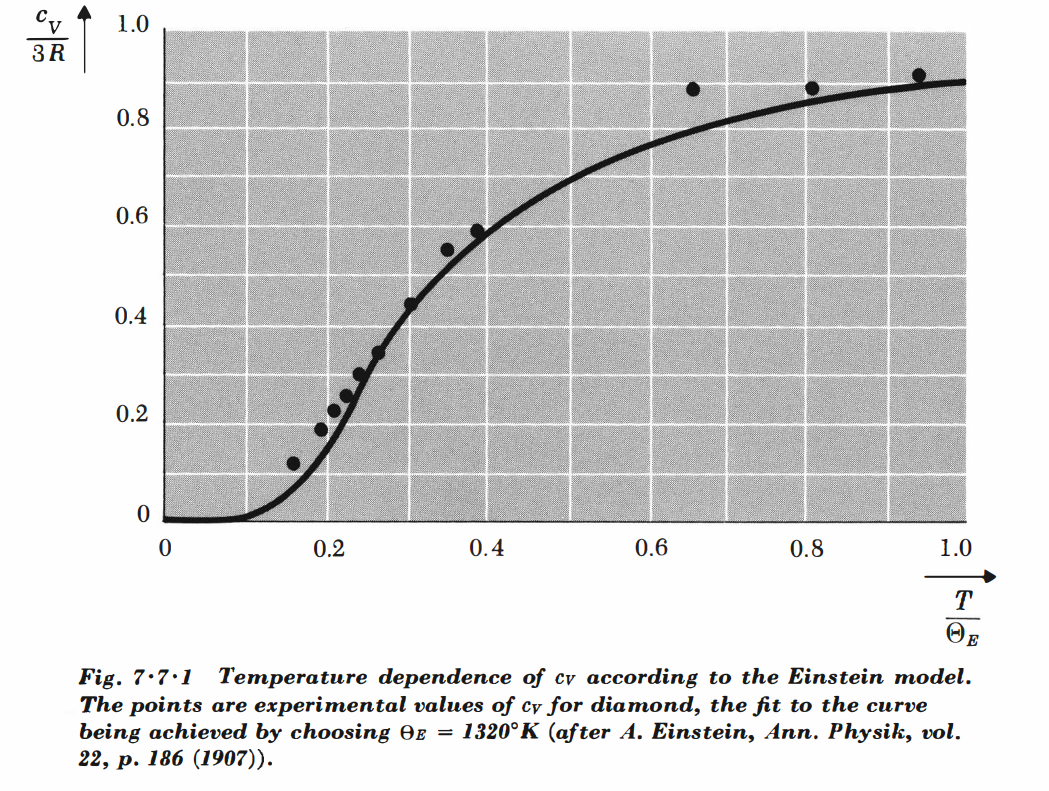
\includegraphics[scale=0.6]{diamond.png}
\end{center}

Note that diamond is hard, the corresponding effective spring constant $k$ is large. So $\hbar \omega$ term is larger for diamond then most other substances because we have:
\begin{align*}
\omega = \sqrt{k/m}
\end{align*}

\newpage
\chapter{Kinetic Theory}
\section[Maxwell Velocity Distribution]{\color{red}Maxwell Velocity Distribution\color{black}}
At a temperature $T$, we want to find the distribution of velocity among the various molecules. Here under a certain set of assumptions, we will get the Maxwell velocity distribution. The assumptions are given by the followings:
\begin{enumerate}
\item The gas is dilute, which means that each molecule in the gas is identifiable, or the molecules are distinguishable and one can follow each without losing track in principle. 
\item The energy of molecule does not depend on its position, but molecules are allowed to have internal energy, such as vibrational and rotational energy. 
\end{enumerate}
Consider a single molecule as a system of interest and the rest of the gas serves as a heat reservoir. We can specify the state of the system of interest by giving $(\vec{r}$, $\vec{p})$ of the single molecule, which gives a point in the phase space with its corresponding internal state. The probability has variables between $\vec{r}$ and $\vec{r}+d\vec{r}$, and between $\vec{p}$ and $\vec{p}+d\vec{p}$, and it has internal state $s$ with energy $E_s$ given by Canonical ensemble. Here we can write:
\begin{align*}
p_s(\vec{r},\vec{p})\, d\vec{r}\, d\vec{p} \propto e^{-\beta\left(\frac{\vec{p^2}}{2m}+E_s\right)}\, d\vec{r}\, d\vec{p}
\end{align*}
where $E_S$ gives energy of rotation and vibration. If we do not care about the internal state of the molecule, then we sum this probability over all internal state which gives us a constant. Now we can write the following:
\begin{align*}
p(\vec{r},\vec{p})\, d\vec{r}\,d\vec{p} \propto e^{-\beta \frac{\vec{p}^2}{2m}}\, d\vec{r}\, d\vec{p}
\end{align*}
Now we integrate over all positions since we only care about the momentum distribution, equivalently the velocity distribution, which is independent of position. Hence we can write the following:
\begin{align*}
p(\vec{p})\, d\vec{p} \propto e^{-\beta \frac{\vec{p}^2}{2m}} \, d\vec{p}
\end{align*}
We note that $\vec{v} = \vec{p}/m$, hence we can write our velocity distribution as the following:
\begin{align*}
p(\vec{v})\, d\vec{v} \propto e^{-\frac{m\vec{v}^2}{2kT}}\, d\vec{v}
\end{align*}
Now we will fix the overall normalization by enforcing that the probability of finding the molecule with any velocity gives us $1$. Let $n = \frac{N}{V}$ be the number of molecules per unit volume. The mean number of molecules with velocity between $\vec{v}$ and $\vec{v}+d\vec{v}$ is given by:
\begin{align*}
f(\vec{v})\,d\vec{v} = nc e^{-\frac{mv^2}{2kT}}\, d\vec{v}
\end{align*}
where $c$ is a constant. $c$ is fixed by the following:
$$nc \int_{\{\text{all possible } \vec{v}\}}  e^{-\frac{mv^2}{2kT}}\,  d\vec{v}= n$$
That is, we have the following:
\begin{align*}
1&= c \int_{-\infty}^\infty\int_{-\infty}^\infty\int_{-\infty}^\infty e^{-\frac{m(v_x^2+v_y^2+v_z^2)}{2kT}}\, dv_x \,dv_y\, dv_z \\
&=c\left( \int_{-\infty}^\infty e^{-\frac{m(v_x^2)}{2kT}}\, dv_x \right)\left( \int_{-\infty}^\infty e^{-\frac{m(v_y^2)}{2kT}}\, dv_y \right)
\left( \int_{-\infty}^\infty e^{-\frac{m(v_z^2)}{2kT}}\, dv_z \right) \\
&= c\left( \int_{-\infty}^\infty e^{-\frac{m(v_x^2)}{2kT}}\, dv_x \right)^3  \\
&= c\left( \frac{2\pi kT}{m}\right)^{3/2}
\end{align*}
Rearranging we get:
$$c= \left( \frac{2\pi kT}{m}\right)^{-3/2} $$
That is, we have:
\begin{align*}
f(\vec{v}) \, d\vec{v} = n  \left( \frac{2\pi kT}{m}\right)^{-3/2}  e^{\frac{-m\vec{v}^2}{2kT}}\, d\vec{v}
\end{align*}
Suppose we are only interested in what the $x$ component of velocity is, irrespective of what the $y$ and $z$ components are. Let $g(v_x)\, dv_x$ be the number of molecules per unit volume with $x$ component of velocity between $v_x$ and $v_x+dv_x$ and $y$ and $z$ components are not measured, so we get:
\begin{align*}
g(v_x)\,dv_x 
&= \int_{\text{all possible }v_y}\int_{\text{all possible }v_z} f(\vec{v})\, d\vec{v}\\
&= n \left( \frac{m}{2\pi kT}\right)^{3/2} e^{-\frac{mv_x^2}{2kT}}\left( \int_{-\infty}^{\infty}e^{-\frac{mv_y^2}{2kT}}\, dv_y \right)\left( \int_{-\infty}^{\infty}e^{-\frac{mv_z^2}{2kT}}\, dv_z \right)\\
&= n \left( \frac{m}{2\pi kT}\right)^{3/2} e^{-\frac{mv_x^2}{2kT}}\left(\frac{2\pi kT}{m}\right)^{1/2}\left(\frac{2\pi kT}{m}\right)^{1/2}\\
&= n\left( \frac{m}{2\pi kT}\right)^{1/2} e^{-\frac{mv_x^2}{2kT}}\,dv_x
\end{align*}
To find the speed distribution. We do not care what solid angle the molecule is going into as long as it has a speed $v$, then $d\vec{v} = v^2 \, dv\, d\Omega$ where $d\Omega = \sin(\theta)d\theta d\phi$ is the solid angle. Let $F(v) \, dv$ be mean number of molecules with speed between $v$ and $v+dv$, then we can rite:
\begin{align*}
F(v)\, dv = \int_{\text{all possible }\Omega} f(\vec{v})\, d\vec{v} = \int_{\text{all possible }\Omega} f(\vec{v})\,v^2 \, dv\, d\Omega
\end{align*}
while $f(\vec{v})$ does not depend on solid angle, hence we get:
\begin{align*}
\int_{\text{all possible }\Omega} f(v)\, d\Omega = 4\pi f(v)
\end{align*} 
Hence we can write:
\begin{align*}
F(v)\, dv = 4\pi v^2 f(v)\, dv = 4\pi v^2 n\left(\frac{m}{2\pi kT}\right)^{3/2} e^{-\frac{mv^2}{2kT}}\, dv
\end{align*}
Now we can write the following, as odd functions integrated to zero:
\begin{align*}
\overline{v_x} = \frac{\int_{-\infty}^{\infty} v_x g(v_x)\, dv_x}{\int_{-\infty}^{\infty} g(v_x) \, dv_x}=0
\end{align*}
For velocity distribution $f(\vec{v})\, d\vec{v}$, the mean value of any function of the form $M(\vec{v})$, is defined by the following:
\begin{align*}
\overline{M(\vec{v})} = \frac{\int_{-\infty}^{\infty} M(\vec{v})\cdot f(\vec{v})\, d\vec{v}}{\int_{-\infty}^{\infty} f(\vec{v})\, d\vec{v}}
\end{align*}
Now we can find the mean value of $v_x^2$:
\begin{align*}
\overline{v_x^2} = \frac{\int_{-\infty}^{\infty} v_x^2 g(v_x)\, dv_x}{\int_{-\infty}^{\infty} g(v_x) d\, v_x}
\end{align*}
The Equipartition Theorem stats that we have:
\begin{align*}
\frac{1}{2}m\overline{v_x^2} = \frac{1}{2}kT \qquad \Rightarrow \qquad \overline{v_x^2 }= \frac{kT}{m}
\end{align*}
One the other hand, we have:
\begin{align*}
\overline{v_x^2} = \frac{\int_{-\infty}^{\infty} v_x^2 g(v_x)\, dv_x}{\int_{-\infty}^{\infty} g(v_x)\, d v_x} &= \left(\frac{m}{2\pi kT}\right)^{1/2} \int_{-\infty}^{\infty} v_x^2 e^{-\frac{mv_x^2}{2kT}}\, dv_x
\end{align*}
Note that we have:
\begin{align*}
\int_{-\infty}^{\infty} v_x^2 e^{av_x^2}\, dv_x = -\frac{\partial }{\partial a}\left(\int_{-\infty}^{\infty} e^{-av_x^2}\, dv_x\right) = -\frac{\partial }{\partial a}\left(\frac{\pi}{a}\right)^{1/2}
\end{align*}
here we take $a = \frac{m}{2kT}$. Hence we get:
\begin{align*}
\overline{v_x^2} &= \left(\frac{m}{2\pi kT}\right)^{1/2}\left( -\frac{\partial}{\partial a}\left(\frac{\pi}{a}\right)^{1/2}\right)\\
&=\left(\frac{m}{2\pi kT}\right)^{1/2}\left( \frac{\sqrt{\pi}}{2}\frac{1}{a^{3/2}}\right) \\
&= \frac{\sqrt{\pi}}{2}\left(\frac{m}{2\pi kT}\right)^{1/2} \left( \frac{2kT}{m}\right)^{3/2}\\
&= \frac{kT}{m} 
\end{align*}

Now we will find the mean speed:
\begin{align*}
\overline{v} = \frac{1}{n}\int_{0}^{\infty} F(v)\,v\, dv = 4\pi \left( \frac{m}{2\pi kT}\right)^{3/2}\int_0^{\infty} v^3 e^{-\frac{mv^2}{2kT}}\, dv = 4\pi \left( \frac{m}{2\pi kT}\right)^{3/2}  \frac{2(kT)^2}{m^2} = \sqrt{\frac{8kT}{m\pi}}
\end{align*}
\hfill\break
\hfill\break
For a distribution, the most probable speed is where the distribution has a maximum. Here we will find the most probable value of $v_x$ distribution. Denote such most probable value as $\widetilde{v}_x$, then we require the following holds:
\begin{align*}
\left.\frac{\partial g(v_x)}{\partial v_x} \right|_{v_x = \widetilde{v}_x} = 0
\end{align*}
so we have:
\begin{align*}
\left.\frac{\partial}{\partial v_x}\left( e^{-\frac{mv_x^2}{2kT}}\right)\right|_{v_x = \widetilde{v}_x} = 0 \qquad \Rightarrow \qquad\left. \frac{mv_x}{kT} e^{-\frac{mv_x^2}{2kT}}\right|_{v_x = \widetilde{v}_x} = 0 \qquad \Rightarrow \qquad \widetilde{v}_x = 0
\end{align*}
Similarly, we can find the most probable speed $\widetilde{v}$:
\begin{align*}
\left.\frac{d}{dv}\left( v^2 e^{-\frac{mv^2}{2kT}}\right)\right|_{v=\widetilde{v}} = 0 \qquad \Rightarrow \qquad \widetilde{v} = \sqrt{\frac{2kT}{m}}
\end{align*}
\hfill\break
Root mean square speed is defined by:
\begin{align*}
v_{rms} = \sqrt{\overline{v^2}} 
\end{align*}
By Equipartition Theorem, we can write the following:
\begin{align*}
\frac{1}{2}m \overline{v^2} = \frac{1}{2}m \overline{v_x^2} + \frac{1}{2}m \overline{v_y^2} + \frac{1}{2}m \overline{v_z^2} = \frac{3}{2}kT
\end{align*}
hence we get:
\begin{align*}
\overline{v^2} = \frac{3kT}{m}\qquad \Rightarrow \qquad v_{rms} = \sqrt{\frac{3kT}{m}}
\end{align*}


The number of molecules per unit volume with velocity between $\vec{v}$ and $\vec{v}+d\vec{v}$ is given by:
\begin{align*}
f(v)\, d\vec{v} = n \lr{\frac{m}{2\pi kT}}^{3/2} e^{-\frac{mv^2}{2kT}}\, dv_x\,dv_y\,dv_z = \frac{ne^{-\frac{mv^2}{2kT}}\, dv_x\,dv_y\,dv_z}{\int_{-\infty}^{\infty}\int_{-\infty}^{\infty}\int_{-\infty}^{\infty} e^{-\frac{mv^2}{2kT}} dv_z \, dv_y \, dv_z}
\end{align*}
\hfill\break
\newpage
\section[Effusion of a Gas]{\color{red} Effusion of a Gas\color{black}}
Effusion is a process which gas leaks out slowly from a container with hole  such that the equilibrium is always maintained inside the container. We want to find the number of particles escaping per unit are per unit time. \\

First we find the number of molecules crossing given area per unit time. Define a coordinate system such that the surface is perpendicular to the $z$-axis. A molecule with velocity $\vec{v}$ will cross $dA$ in time $dt$. So the number of molecules crossing area $dA$ in time $dt$ is given by the following:
\begin{align*}
f(\vec{v})\, d\vec{v} \, v_z \, dt \, dA
\end{align*}
The flux is defined by:
\begin{align*}
\text{Flux} = \frac{\text{number crossing the surface}}{dA\cdot dt} = v_z \, f(\vec{v})\, d\vec{v}
\end{align*}
The total flux through $dA$ from the left is given by:
\begin{align*}
\int_{v_z >0}\, v_z f(\vec{v})\, dv_x\,dv_y\, dv_z &= \frac{n \int_0^{\infty}v_z e^{-\frac{mv_z^2}{2kT}}\,dv_z \int_{-\infty}^{\infty} e^{-\frac{mv_y^2}{2kT}}\, dv_y \int_{-\infty}^{\infty} e^{-\frac{mv_x^2}{2kT}}\, dv_x}{ \int_{-\infty}^{\infty}v_z e^{-\frac{mv_z^2}{2kT}}\,dv_z \int_{-\infty}^{\infty} e^{-\frac{mv_y^2}{2kT}}\, dv_y \int_{-\infty}^{\infty} e^{-\frac{mv_x^2}{2kT}}\, dv_x}\\
&= n \frac{\int_0^{\infty}v_z e^{-\frac{mv_z^2}{2kT}}\,dv_z }{\int_{-\infty}^{\infty}v_z e^{-\frac{mv_z^2}{2kT}}\,dv_z } \\
&= n \frac{\int_0^{\infty} e^{-\frac{mv_z^2}{2kT}}\, d\lr{\frac{1}{2}v_z^2}}{\int_{-\infty}^{\infty}e^{-\frac{mv_z^2}{2kT}}\, dv_z}\\
&= n \frac{\int_0^\infty e^{-\frac{ym}{kT}}\, dy}{\lr{\frac{2\pi kT}{m}}^{1/2}}\\
&= \frac{\frac{nkT}{m}}{\sqrt{\frac{2\pi kT}{m}}} \\
&= n \sqrt{\frac{kT}{2m \pi}} \\
&= \frac{n}{4}\bar{v}
\end{align*}

\newpage
\section[Pressure of a Gas]{\color{red} Kinetic Theory for the Calculation of Pressure\color{black}} 
Consider area $dA$ of the container wall, perpendicular $z$-axis. Particles strike the wall and get scattered back. Momentum transferred to the wall due to molecules of velocity $\vec{v}$ is given by:
\begin{align*}
(2mv_z)(v_z\,dA\,dt)(f(\vec{v})\,d\vec{v})
\end{align*}
where $2mv_z$ gives the momentum transfer of each molecule, $(v_z\,dA\,dt)(f(\vec{v})\,d\vec{v})$ gives the number of molecules with velocity $\vec{v}$ that strikes the wall in time $dt$. The pressure is given by:
\begin{align*}
\text{Pressure} = \frac{\text{momentum transfer}}{\text{time} \cdot \text{area}} = 2mv_z^2 f(\vec{v})\, d\vec{v}
\end{align*}
The total pressure exerted on the wall is given by the following:
\begin{align*}
p &= \int_{v_z>0}2mv_z^2\, f(\vec{v})\, d\vec{v} \\
&= \frac{1}{2}\int_{\text{all possible } \vec{v}} 2mv_z^2\, f(\vec{v})\, d\vec{v}\\
&=\int_{\text{all possible } \vec{v}} mv_z^2 f(\vec{v})\, d\vec{v}\\
&= n m\overline{v_z^2}\\
&= 2n \cdot \frac{1}{2}m \overline{v_z^2}\\ 
&= 2n \left( \frac{1}{2}kT
\right) \\
&= nkT
\end{align*}
Here we get the ideal gas law from kinetic theory:
\begin{align*}
p = \frac{NkT}{V}
\end{align*}



\newpage
\chapter{Equilibriums}

\section[Equilibrium Conditions for Systems]{\color{red}Equilibrium Conditions for Systems\color{black}}
Now we want to find equilibrium conditions under different situations.
\begin{enumerate}[topsep=3pt,itemsep=-1ex,partopsep=1ex,parsep=1ex]
\item Isolated system
\item System in contact with temperature and pressure reservoirs
\end{enumerate}
Here we can find a formulation of equilibrium condition in terms of entropy or other thermodynamics potentials.  \\


First we consider the isolated system. For any spontaneously occurring process in an isolated system, we know that $\Delta S \geq 0$ by the Second Law of Thermodynamics. Hence we have:
\begin{center}
\textit{Equilibrium of the isolated system is characterized by having the maximum of the entropy.}
\end{center} 
Important fundamental relation of such situation is characterized by $S$ being a function of $E$, $V$, and internal or external parameters $y_1,y_2.\cdots. y_n$. Most physical systems are not isolated, they are in contact with temperature and pressure reservoirs.\\

For the systems in contact with temperature and pressure reservoirs, the fundamental relation is given in terms of $G(T,p, y_1,y_2,\cdots,y_n)$, the Gibbs Free Energy, or $F(T,V,y_1,y_2,\cdots, y_n)$, the Helmholtz Free Energy, where $y_1,y_2,\cdots, y_n$ are internal or external parameters. We want to translate the condition $\Delta S \geq 0$ into a statement about $G$ and $F$ for systems in contact with pressure and temperature reservoirs in order to find the equilibrium condition for system in contact with temperature and pressure reservoir. At such equilibrium, again, $S$ is at maximum.\\

Consider the following situation. 
\begin{center}
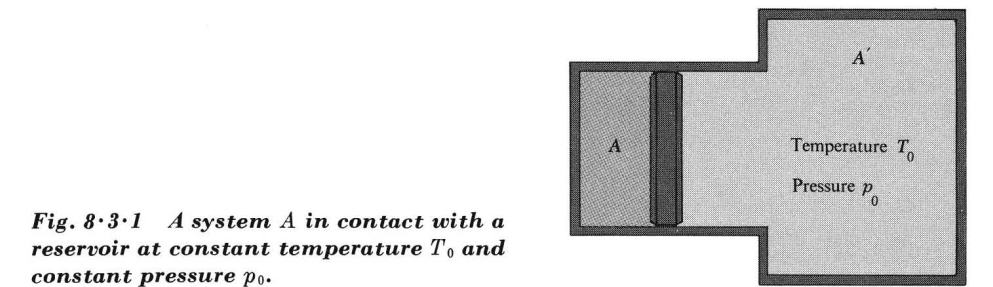
\includegraphics[scale=0.5]{eqAA'.png}
\end{center}
Here we have an isolated system, there is a reservoir with temperature $T_0$ and pressure $p_0$. A subsystem $A$ is in contact with the reservoir, and $A$ is connected to a work source. Consider a general situation when system $A$ changes state, possibly exchanging heat with the reservoir, or doing work in the process. Here we want to find the amount of work $W^*$ that can be done on a work source by $A$. Now we denote system $A$ does work $W^*$, the energy of the subsystem $A$ increases by $\Delta E$, volume increases by $\Delta V$, and entropy changes by $\Delta S$. Here we note that work source is always thermally isolated. For the reservoir, volume increases in $\Delta V_0 = -\Delta V$, and entropy increases in $\Delta S_0$. The First Law of Thermodynamics states the following:
\begin{align*}
W^* + \Delta E - p_0 \Delta V_0 + T_0 \Delta S_0 = 0 \tag{*}
\end{align*}
Note here $p_0 \Delta V_0 =- p_0 \Delta V$ denotes the amount of work done by $A$ to the reservoir $A'$, and $W^*$ denotes the amount of work done by $A$ to the work source only. The Second Law of Thermodynamics states the following:
\begin{align*}
\Delta (S + S_0) \geq 0 \qquad \qquad \Rightarrow \qquad \qquad \Delta S_0 \geq - \Delta S\tag{**}
\end{align*}
combing (*), (**), and $\Delta V_0 = -\Delta V$, we get the following:
\begin{align*}
W^* + \Delta E + p_0 \Delta V - T_0 \Delta S \leq 0 \qquad \Rightarrow \qquad W^* \leq -\Delta E - p_0 \Delta V + T_0 \Delta S
\end{align*}
Since $p_0$ and $T_0$ are constants, then we can write:
\begin{align*}
W^* \leq -\Delta (E - T_0 S + p_0 V) \tag{AW}
\end{align*}
The general result is characterized by equation (AW). Here we can define $G_0 = E - T_0 S + p_0 V$, hence $-\Delta  (E - T_0 S + p_0 V)  = -\Delta G_0$. Here $G_0$ is not the Gibbs Free Energy of $A$ because $T_0$ and $p_0$ refer to parameters of the reservoir, not parameters of $A$.\\

Now consider some special cases, system $A$ starts and ends at $T=  T_0$, $p=p_0$, then $W^* \leq -\Delta (E - TS + pV) = -\Delta G$, where $G$ is the real Gibbs Free Energy of system $A$.\\

Consider another special case, where system $A$ has a fixed volume, $\Delta V = 0$, then we know that $W^* = -\Delta (E - T_0 S) = -\Delta F_0$. If $T = T_0$, then $W^* \leq -\Delta F$ where $F$ is the Helmholtz Free Energy of subsystem $A$. In this case, we have $W^* \leq -\Delta G$ and $W^* \leq -\Delta F$ for fixed volume. Hence $-\Delta G$ and $-\Delta F$ represents the maximum amount of work that can be done by system $A$. This explains why $G$ and $F$ are called the Free Energies. \\

Now consider the case where the process is a spontaneously occurring process, that is, we have $W^* = 0$. Then we can write $0 \leq -\Delta G_0$ or $\Delta G_0 \leq 0$, which implies $G_0$ decreases in such process. For a system with fixed volume, we have further that $\Delta F_0 \leq 0$. \\

Here we see that the equations $\Delta F_0 \leq 0$ and $\Delta G_0 \leq 0$ are analog to the equation $\Delta S \geq 0$, and $\Delta S \geq 0$ gives us a way to characterize the equilibrium of an isolated system. Now we can conclude: 
\begin{center}
\textit{For equilibrium in system $A$ in contact with a temperature and pressure reservoir, $G_0$ is minimized. If we have further that volume of $A$ being fixed, $F_0$ is minimized at equilibrium.}
\end{center}
This is an analogue of $S$ be maximized for isolated system to be in equilibrium. \\

Now we want to look at the stability of a thermodynamics system. Subsystem $A$ is in contact with a reservoir with temperature $T_0$ and pressure $p_0$, system $A$ along with the reservoir are in an isolated system. We want to see whether fluctuation about equilibrium position increase or decrease $G_0$. If the fluctuation decreases $G_0$, then the equilibrium is an unstable equilibrium, and otherwise if the fluctuation increases $G_0$, then the equilibrium is a stable equilibrium. We will characterize the state of $A$ by giving $T$ and $V$. For the extremum, we have:
\begin{align*}
\lr{\frac{\partial G_0}{\pd T}}_V  = 0 \qquad\qquad\qquad \lr{\frac{\pd G_0}{\pd V}}_T = 0 \tag{EQG}
\end{align*}
now we expand about the minimum $G_{min}$:
\begin{align*}
G_0 = G_{min} + \frac{1}{2}\lr{\frac{\partial^2 G_0}{\partial T^2}}_V \lr{\Delta T}^2 +  \frac{1}{2}\lr{\frac{\partial^2 G_0}{\partial V^2}}_T \lr{\Delta V}^2 + \left.\lr{\frac{\partial^2 G_0}{\pd T \pd V}}\right|_{\text{at eq.}}\lr{\Delta T \,\Delta V} + \cdots
\end{align*}
there is no linear terms in Taylor expansion because we have equation (EQG) holds. Here we have:
\begin{align*}
G_0 = E - T_0 S + p_0 V
\end{align*}
hence we can write:
\begin{align*}
 \lr{\frac{\pd G_0}{\pd T}}_V = \lr{\frac{\pd E}{\pd T}}_V -T_0 \lr{\frac{\pd S}{\pd T}}_V = T\lr{\frac{\pd S}{\pd T}}_V - T_0 \lr{\frac{\pd S}{\pd T}}_V \tag{1}
\end{align*}
Here we see that, at equilibrium, we have the following:
\begin{align*}
0 = \lr{\frac{\pd G_0}{\pd T}}_V \qquad \Rightarrow \qquad T = T_0
\end{align*}
With equation (1), we can write:
\begin{align*}
\lr{\frac{\pd^2 G_0}{\pd T^2}}_V = T\lr{\frac{\pd^2 S}{\pd T^2}}_V + \lr{\frac{\pd S}{\pd T}}_V - T_0 \lr{\frac{\pd^2S}{\pd T^2}}_V
\end{align*}
when we have $T = T_0$, we see that we have the following holds:
\begin{align*}
\lr{\frac{\pd^2 G_0}{\pd T^2}}_V  = \lr{\frac{\pd S}{\pd T}}_V = \frac{C_V}{T_0}
\end{align*}
Moreover, with equation (1), we can write:
\begin{align*}
\frac{\pd^2 G_0}{\pd T \pd V} = T \frac{\pd^2 S}{\pd T \pd V} - T_0 \frac{\pd^2 S}{\pd T \pd V} 
\end{align*}
at $T = T_0$, we get:
\begin{align*}
\frac{\pd^2 G_0}{\pd T \pd V} = 0
\end{align*}
On the other hand, we have:
\begin{align*}
\lr{\frac{\pd G_0}{\pd V}}_T = \lr{\frac{\pd E}{\pd V}}_T - T_0 \lr{\frac{\pd S}{\pd V}}_T + p_0 = T\lr{\frac{\pd S}{\pd V}}_T - p - T_0 \lr{\frac{\pd S}{\pd V}}_T + p_0
\end{align*}
when at equilibrium, we have have the following holds:
$$\lr{\frac{\pd G_0}{\pd V}}_T = 0 \qquad\Rightarrow\qquad p= p_0 \quad \text{at}\quad T = T_0$$ 

At equilibrium, we have $T = T_0$ and $p= p_0$, and hence we get:
\begin{align*}
\lr{\frac{\pd^2 G_0}{\pd V^2}}_T = T \lr{\frac{\pd^2 S}{\pd V^2}}_T - \lr{\frac{\pd p}{\pd V}}_T - T_0 \lr{\frac{\pd^2 S}{\pd V^2}}_T =-\lr{\frac{\pd p}{\pd V}}_T = \frac{1}{V\kappa}
\end{align*}
so now we get:
\begin{align*}
G_0 = G_{min} + \frac{C_V}{2T_0} \lr{\Delta T}^2 + \frac{1}{2V\kappa}\lr{\Delta V}^2
\end{align*}
Here we see that, for stability, we require the following holds:
\begin{align*}
\frac{C_V}{2T_0} \lr{\Delta T}^2 + \frac{1}{2V\kappa}\lr{\Delta V}^2 >0
\end{align*}
and hence the system equilibrium is stable if we have both $C_V > 0$ and $\kappa >0$. \\

\newpage
\section[Phase Transition]{\color{red}Phase Transition\color{black}}
Phase Transition is an application of study of thermodynamic instability. A system is thermodynamically stable, as we derived in the previous section, if $C_V>0$ and $\kappa >0$. \\

Matter can exist in different phase: solid, liquid, and gas. Phase transition is what leads to the preference of one phase over a another and is when different phases can co-exist.\\

We will see that the prediction of thermodynamic instability may imply the existence of two phases which may co-exist under certain circumstances. \\

\example
Superconductor and normalconductor are also topics in phase transition.\\

The phase transitions are induced by thermodynamics instability. For ideal gas, there is no phase transition because $\kappa = 1/p$ is always positive. But Van der Waals gas does have phase transition. For $1$-model of Van der Waals gas, we have:
\begin{align*}
\left( p + \frac{a}{V^2}\right) (V-b) = RT
\end{align*}
\hfill\break\hfill\break
\begin{center}
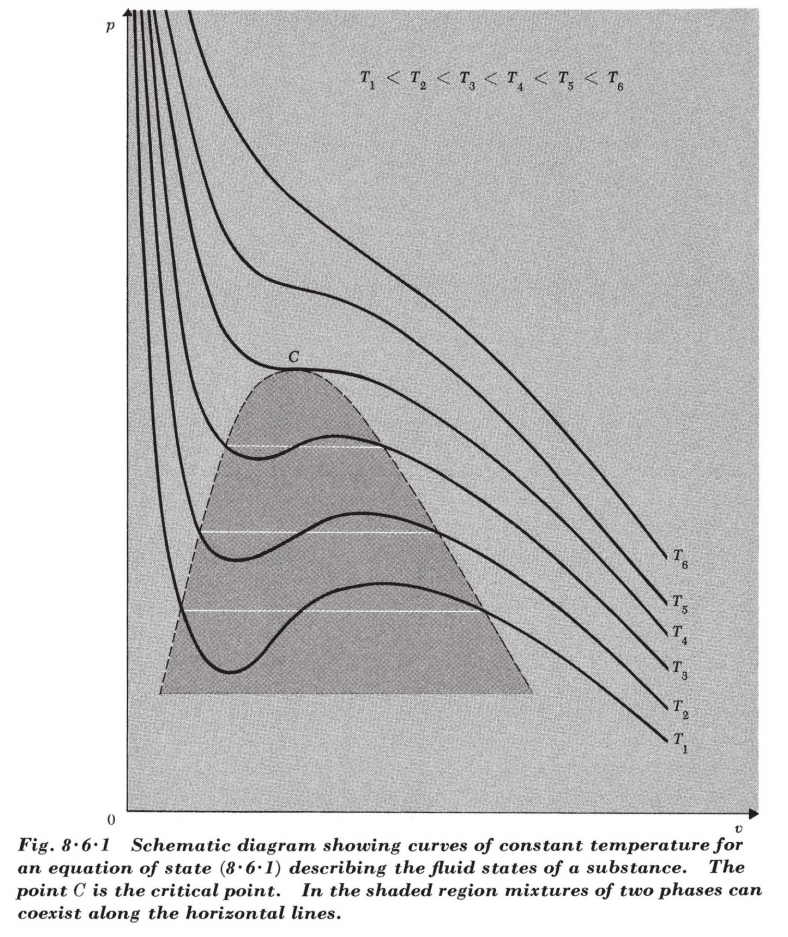
\includegraphics[scale=0.69]{phase1.png}\\
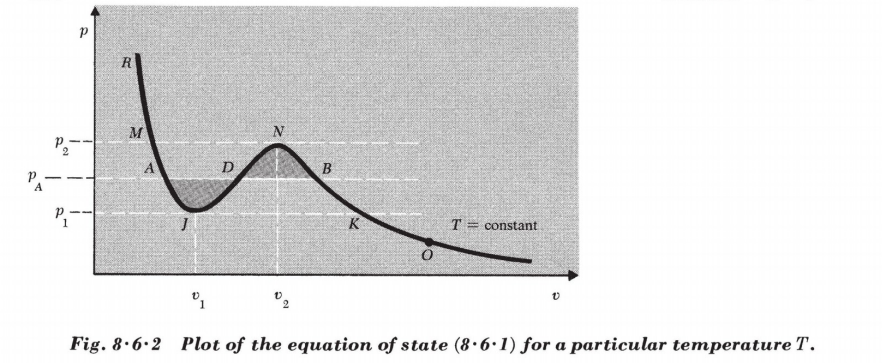
\includegraphics[scale=0.69]{phase2.png}
\end{center}
Between $J$ and $N$, the calculated isotherms predict that we have $\lr{\frac{\partial p}{\partial V}}_T >0$, or $\kappa <0$. Hence the Van der Waals gas undergoes a phase change between liquid and gas.\\


\hfill\break\hfill\break
Now consider a system with molecules of two phases in contact with $T$ reservoir and $P$ reservoir. Let $G$ be the Gibbs Free Energy of the system, let $g_i(T,p)$ be the Gibbs Free Energy for $1$ mole for molecules in phase $i$, let $\nu_i$ be the number of molecules in the phase $i$. At equilibrium we require the following holds:
\begin{align*}
G = \nu_1 g_1 + \nu_2 g_2 = minimum
\end{align*}
and we have a constraint that: 
$$\nu_1 + \nu_2 = \nu$$
where $\nu$ is a given number being the total number of molecules in two phases, $\nu_1$ and $\nu_2$ may vary. For given $p$ and $T$, here we have three possibilities:\\
(1) $g_1(T,p) < g_2(T,p)$, at equilibrium, the minimum of $G$ occurring at $G = \nu g_1$, all in phase $1$.\\
(2) $g_1(T,p) > g_2(T,p)$, at equilibrium, the minimum of $G$ occurring at $G = \nu g_2$, all in phase $2$.\\
(3) $g_1(T,p) = g_2(T,p)$, at equilibrium, arbitrary amounts of $\nu_1$ and $\nu_2$ can coexists with $\nu_1 + \nu_2 = \nu$.\\

The phase diagram for such configuration is a $pT$-diagram. \\
A line on the diagram for two phases defined by $i$ and $j$ specifies the values of $p$ and $T$ for which we have $g_i = g_j$, and the line separates the two phases. 
\begin{center}
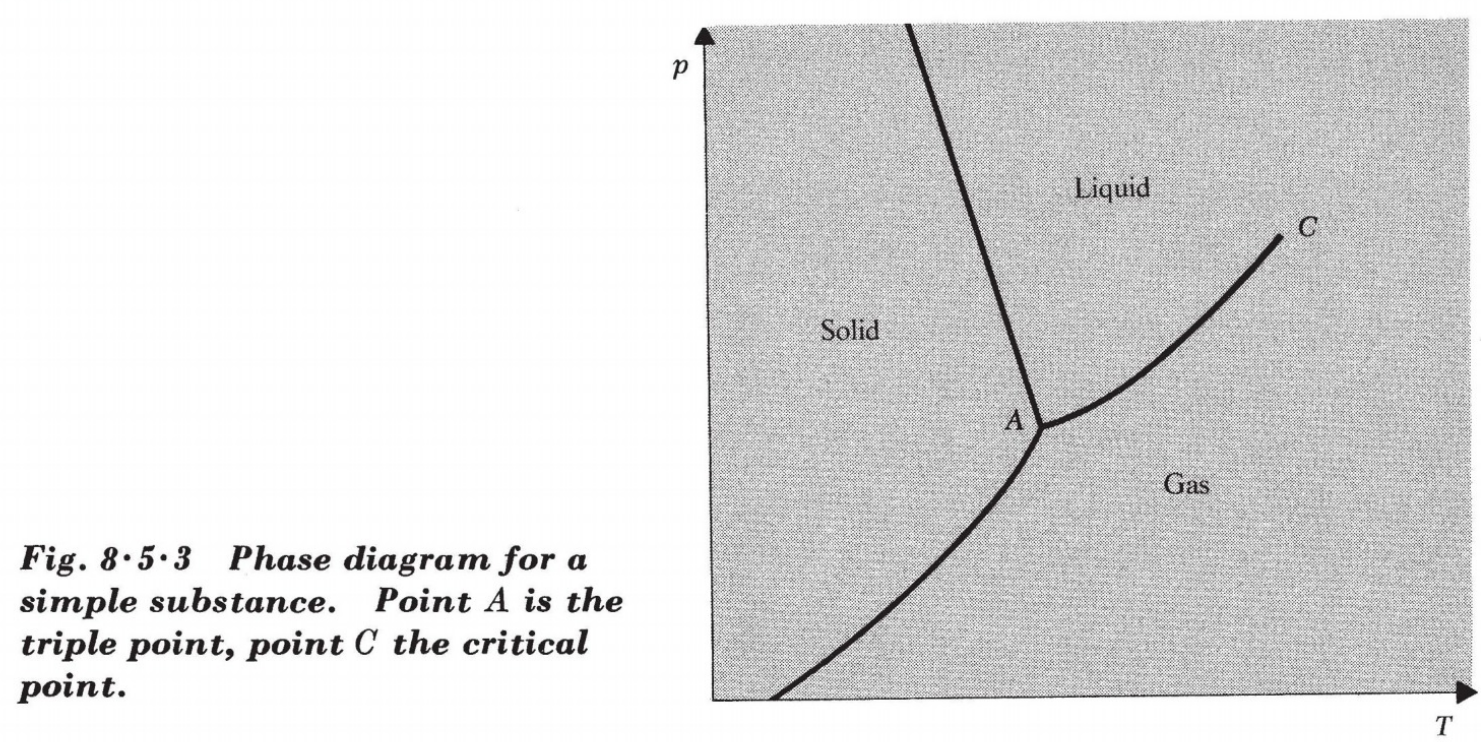
\includegraphics[scale=0.35]{phaseDiagm.png}
\end{center}
Here $C$ is a critical point, beyond which there is no phase transition due to high pressure and temperature, and it is hard to distinguish between gas and liquid.\\

Note that there is change in internal energy during a phase transition, at such process, we have given $T$ and $p$, let $E_i$ denote the energy of the systems with particles in phase $i$, and $S_i$ and $V_i$ denote the entropy and volume of the systems of particles in phase $i$, respectively, we can write:
\begin{align*}
g_1 &= g_2 \\
E_1 - T S_1 + pV_1 &= E_2 - T S_2 + pV_2 \\ 
\end{align*}
Rearranging we get the following:
\begin{align*}
(E_1 - E_2) - T(S_1 - S_2) + p(V_1 - V_2) = 0
\end{align*}
Here $T(S_1 - T_2)$ is the amount of Latent Heat absorbed, and $p(V_1 - V_2)$ is the amount of work done. \\

\subsection{First Order Phase Transition}
Examples for the first order phase transition include going from liquid to gas, from gas to liquid, but except for the conductor example given above. Denote $g(T,p)$ be the Gibbs Free Energy of the system, first order transitions are characterized by $g$ being continuous around the boundary between phases, with the first partial derivative of $g$ being discontinuous around the boundaries between phases. \\

Note that we have the following quantities by definition:
\begin{align*}
\lr{\frac{\pd g}{\pd p}}_T = v \qquad\qquad\qquad \lr{\frac{\pd g}{\pd T}}_p = -s
\end{align*}
where $v$ is the molar volume, and $s$ is the molar entropy. In first order phase transitions, molar volume changes, and the Latent Heat is absorbed or given off, in which case entropy changes.\\

In first order phase transition, here $g_1 = g_2$, in differential form we have $dg_1 = dg_2$, where we can write:
\begin{align*}
\lr{\frac{\pd g_1}{\pd p}}_T \, dp + \lr{\frac{\pd g_1}{\pd T}}_p \, dT =\lr{\frac{\pd g_2}{\pd p}}_T \, dp + \lr{\frac{\pd g_2}{\pd T}}_p \, dT  
\end{align*}
\begin{align*}
\Delta \lr{\frac{\pd g}{\pd p}}_T \, dp = -\Delta \lr{\frac{\pd g}{\pd T}}_p\, dT \tag{*}
\end{align*}
where:
\begin{align*}
\Delta \lr{\frac{\pd g}{\pd p}}_T = \lr{\frac{\pd g_1}{\pd p}}_T - \lr{\frac{\pd g_2}{\pd p}}_T\qquad\qquad \Delta \lr{\frac{\pd g}{\pd T}}_p = \lr{\frac{\pd g_1}{\pd T}}_p - \lr{\frac{\pd g_2}{\pd T}}_p
\end{align*}
Here we have:
\begin{align*}
\Delta \lr{\frac{\pd g}{\pd p}}_T = v_1 - v_2 = \Delta v = \text{change in molar volume of the two phases}
\end{align*}
\begin{align*}
\Delta \lr{\frac{\pd g}{\pd T}}_p = -(s_1 - s_2) = -\Delta s = \text{change in molar entropy of the two phases} 
\end{align*}
Since molar entropies are different, some amount of heat must be absorbed by one phase relative to the other, which is called the Latent Heat. In particular, in our deviation, Latent heat is defined as the heat absorbed when a given amount of phase 2 is transformed to phase 1, denote the Latent heat as $L_{21}$. Note that the Latent heat is measured in total amount instead of molar amount, hence we write:
\begin{align*}
\Delta S \coloneqq \frac{L}{T}
\end{align*}
Hence from equation (*), both numerator and denominator can be multiplied by the same number of moles, and hence we get the following:
\begin{align*}
\frac{dp}{dT} = \frac{\Delta S}{\Delta V} = \frac{L}{T\Delta V} \tag{CC}
\end{align*}
Equation (CC) is called the Clausius-Clapeyron Equation. \\


\subsection{Second Order Phase Transition}
In second order phase transition, both $g$ and first order derivative of $g$ are continuous around the boundary between phases, but the second order derivatives are not continuous around the phase boundaries. Hence there is no Latent heat for second order phase transition. 

\subsection{Application of Clausius-Clapeyron Equation}
Consider liquid-vapor phase transition. We want to find the pressure of the vapor in equilibrium with liquid at a given temperature $T$. First note that we can write the following by the Clausius-Clapeyron Equation:
\begin{align*}
\frac{dp}{dT} = \frac{L}{T \Delta V}
\end{align*}
Here we note that we make the following assumption:
\begin{align*}
\Delta V = V_{vapor} - V_{liquid} \approx V_{vapor}\qquad\qquad \text{because we have }V_{liquid}<<V_{vapor}
\end{align*}
For the vapor, we assume it to be ideal, that is, we have $pV = RT$. Here we also assume that $L$ is independent of $T$.\\

Now we can write:
\begin{align*}
\frac{dp}{dT} = \frac{L}{T} \frac{1}{V_{vapor}} = \frac{L}{T} \frac{p}{RT} = \frac{Lp}{RT^2} \qquad \Rightarrow \qquad \frac{dp}{p} = \frac{L dT}{RT^2} \qquad \Rightarrow \qquad \ln(p) = -\frac{L}{RT} + C
\end{align*}
where $C$ is a constant, rearranging we get the following:
\begin{align*}
p = p_0 e^{-\frac{L}{RT}} \tag{PC}
\end{align*}
where $p_0$ is a constant. Equation (PC) gives the pressure, called the vapor pressure, of the liquid at this equilibrium, and equation (PC) states that, as the temperature is lowered, the pressure falls exponentially.\\

\newpage
\section[Chemical Potential]{\color{red}Chemical Potential \color{black}}
In general, $S$ is a function of $E$, $V$, and $N$. So far in our discussion, $N$ has been treated to be a constant, but in some processes, $N$ may vary instead, examples that $N$ varies include chemical reactions, semi-permeable membrane, and phase transition. If $E$, $V$, and $N$ all vary, we can write the following:
\begin{align*}
dS = \lr{\frac{\pd S}{\pd E}}_{V,N} \, dE +  \lr{\frac{\pd S}{\pd V}}_{E,N} \, dV +  \lr{\frac{\pd S}{\pd N}}_{E,V} \, dN = \frac{1}{T}\, dE + \frac{p}{T}\, dV + \lr{\frac{\pd S}{\pd N}}_{E,V} \, dN \tag{CPS}
\end{align*}
Here we define:
\begin{align*}
\lr{\frac{\pd S}{\pd N}}_{E,V} \coloneqq - \frac{\mu}{T}
\end{align*}
here the $\mu$ is called the chemical potential per molecule. On the other hand, we can write:
\begin{align*}
dE = T\, dS - p\, dV + \mu \, dN
\end{align*}

Here we will investigate the general condition for equilibrium. Consider a system with two subsystems, each with parameters $E_i, V_i, N_i$ representing energies, volumes, and number of molecules, for $i=1$ and $i=2$, respectively. Partition between the two subsystems is thermally conducting, movable, and porous. Here we have $E_1 + E_2 \coloneqq E^0$ being constant, and $N_1 + N_2 = N_0$ being fixed. Then we can write:
\begin{align*}
S= S_1 (E_1,V_1,N_1) + S_2(E_1,V_1,N_2)
\end{align*}
where $S_1$ and $S_2$ represent the entropy of the two subsystems. In equilibrium, $S$ has to be at maximum. As derived previously, we must have the followings holds:
\begin{align*}
\frac{\pd S}{\pd E_1} = 0 \qquad \Rightarrow \qquad T_1 = T_2
\end{align*}
\begin{align*}
\frac{\pd S}{\pd V_1}= 0 \qquad \Rightarrow \qquad p_1 = p_2
\end{align*}
Now we also require the following holds:
\begin{align*}
\frac{\pd S}{\pd N_1} = \frac{\pd S_1}{\pd N_1} + \frac{\pd S_2}{\pd N_1} = \frac{\pd S_1}{\pd N_1} - \frac{\pd S_2}{\pd N_2} = 0
\end{align*}
in which case we have:
\begin{align*}
-\frac{\mu_1}{T_1} + \frac{\mu_2}{T_2} = 0 \qquad \Rightarrow \qquad \mu_1 = \mu_2 \text{ at equilibrium}
\end{align*}

Now we consider $E_i$ and $V_i$ are kept fixed, then we can write the following:
\begin{align*}
dS = \frac{\pd S}{\pd N_1}\,dN_1 = \left( - \frac{\mu_1}{T_1}+ \frac{\mu_2}{T_2}\right) \, dN_1 \geq 0
\end{align*}
Assume $T_1 = T_2$, in a spontaneous process, if we have $\mu_1 > \mu_2$, then $dN_1 < 0$. \\
This shows that particles flow from high $\mu$ to low $\mu$.\\

On the other hand, by equation (CPS) we can write:
\begin{align*}
dS = \frac{1}{T}\, dE + \frac{p}{T}\, dV - \frac{\mu}{T}\, dT
\end{align*}
rearranging we get:
\begin{align*}
dE = T\, dS - p\, dV + \mu\, dN \qquad \Rightarrow \qquad 
\mu = \lr{\frac{\pd E}{\pd N}}_{S,V} 
\end{align*}
Note that we can interchange the independent variable $S$ to $T$, and $E$ to $F$, then we have:
\begin{align*}
dF = -S\, dT - p\, dV + \mu\, dN \qquad \Rightarrow \qquad \mu = \lr{\frac{\pd F}{\pd N}}_{T,V}
\end{align*}
Now we further change variable from $V$ to $p$, then we get, and $F$ to $G$:
\begin{align*}
dG = -S\, dT + V\, dp + \mu\, dN \qquad \Rightarrow \qquad \mu = \lr{\frac{\pd G}{\pd N}}_{T,p}
\end{align*}

\subsection*{Gibbs Free Energy and Chemical Potential}
Suppose there is only one species of molecules, then we can write:
\begin{align*}
G(T,p, N) = N \, g'(T,p)
\end{align*}
which is the only way that $N$ can be an extensive quantity. Here $g'(T,p)$ is the Gibbs Free Energy per molecule. Note here we have:
\begin{align*}
\mu = \lr{\frac{\pd G}{\pd N}}_{T,p} = g'(T,p)
\end{align*}
where we see now $\mu$ is an intensive quantity, hence it can only depend on the ratios of extensive quantities, such as $V/N$ and $S/N$. If there is only one specie of molecules, then we identity $\mu$ as the Gibbs Free Energy per molecule.\\

If there are several species of molecules, each with number of molecules $N_i$ for some indexing $i$, then we can write:
\begin{align*}
G = G(T,p, N_1, N_2, \cdots, N_n)
\end{align*}
for each specie we can define a chemical potential: 
$$\mu_j = \lr{\frac{\pd G}{\pd N_j}}_{T,P, N_1,\cdots, N_{j-1}, N_{j+1}, \cdots, N_n}$$
note here $\mu_j$ can be a function of $N_1/N_2$ if $j \neq 1$ and $j \neq 2$. \\

\subsection*{Ideal Gas and Chemical Potential}
Here we can write the following from previous discussion:
\begin{align*}
F = -kT\ln(z) \qquad \Rightarrow \qquad \mu = \lr{\frac{\pd F}{\pd N}}_{T,V} = -kT \lr{\frac{\pd (\ln(z))}{\pd N}}_{T,V}
\end{align*}
we have seen that for an ideal gas, we have:
\begin{align*}
z = \frac{\rho^N}{N!}
\end{align*}
where $\rho$ is the partition function for one particle, and hence we have:
\begin{align*}
\ln(z) = N \ln (\rho) - \ln(N!) \approx N \ln(\rho) - N \ln(N) + N
\end{align*}
Now we can write:
\begin{align*}
\mu = -kT(\ln(\rho) - \ln(N) - 1 + 1) = -kT \ln\lr{\frac{\rho}{N}}
\end{align*}
Now consider $\rho(V,E)$ for one molecule of ideal gas, since $E$ only depends on $T$ for ideal gas, we can write the following:
\begin{align*}
\rho(V,E) = V\rho'(E) = V\rho''(T)
\end{align*}
for some functions $\rho'$ and $\rho''$, so we have:
\begin{align*}
\mu = -kT \left( \ln\lr{\frac{V}{N}} + \ln(\rho'')\right)
\end{align*}
here we see that $\mu$ depends on ratios of extensive quantities, and we also see that $\mu$ increase with concentration defined by $N/V$. 
\newpage

\section[Grand Canonical Ensemble]{\color{red} Grand Canonical Ensemble\color{black}}
Consider a system $A$ in contact with temperature and particle reservoir $A'$ of chemical potential $\mu_0$ and temperature $T_0$. Note here $A$ has fixed external parameters and can exchange both heat and number of particles with $A'$. Here $A$ can be decided by a grand canonical ensemble, which includes the description of different energy states $E_r$ and number of particles $N_r$.\\

The combined system $A + A' = A_0$ is isolated, so $E+E' = E_0$ is a constant, and $N + N' = N_0$ is also fixed. Consider now a specific state $r$ for system $A$, with energy $E_r$ and number of particles $N_r$. The probability of such state, denoted as $p_r(E_r,N_r)$, is given by the following:
\begin{align*}
p_r(E_r, N_r) = \Omega \cdot \Omega'(E_0 - E_r, N_0 - E_r)
\end{align*}
$\Omega = 1$ because $A$ is assumed to be one specific state. Here we can write:
\begin{align*}
\ln(\Omega'(E_0 - E_r, N_0 - E_r)) &= \ln(\Omega' (E_0, N_0)) - \lr{\frac{\pd \ln(\Omega')}{\pd E'}}E_r - \lr{\frac{\pd \ln(\Omega')}{\pd N'}}N_r + (\text{higher order terms})\\
&\approx \text{constant}  -\beta' E_r -\alpha' N_r
\end{align*}
where we have, denoting $T'$ as the temperature of the reservoir, and $\mu'$ as the chemical potential of the reservoir:
\begin{align*}
\beta ' = \frac{1}{kT'} \qquad\qquad \qquad \alpha' \coloneqq \frac{\pd \ln(\Omega')}{\pd N'} = -\frac{\mu'}{kT'}
\end{align*}
so we can write:
\begin{align*}
p_r \propto e^{-\beta ' E_r - \alpha' N_r}
\end{align*} 
at equilibrium, we have $T'= T$, and $\mu' = \mu$. \\

One can also derive the grand canonical ensemble in another approach. The probability distribution is one that maximizes missing information. Here at equilibrium, we want to maximize the following:
$$S = -k \sum_r p_r \ln(p_r)$$ 
under the constraint:
\begin{align*}
\sum_r p_r E_r = \bar{E} \qquad \qquad \sum_r N_r p_r = \bar{N} \qquad\qquad \sum_r p_r = 1
\end{align*} 
By Lagrange Multiplier Theorem, we can write:
\begin{align*}
\frac{\pd}{\pd p_j} \left( -\sum_r p_r \ln(p_r) - \beta \sum_r p_r E_r - \alpha \sum_r p_r N_r - \gamma \sum_r p_r \right) &= 0\\
 -(\ln p_j +1) - \beta E_j - \alpha N_j - \gamma &= 0
\end{align*}
Rearranging we get:
\begin{align*}
\ln(p_j) = -(\gamma+1) -\beta E_j - \alpha N_j
\end{align*} 
hence we have:
\begin{align*}
p_j = e^{\gamma+1} e^{-\beta E_j} e^{-\alpha N_j}
\end{align*}
We fix $\alpha$ such that we have the following:
\begin{align*}
\frac{\sum_j N_j e^{\beta E_j - \alpha N_j}}{\sum_j e^{\beta E_j - \alpha N_j}} = 1
\end{align*} 
and fix $\beta$ such that we have:
\begin{align*}
\frac{\sum_j E_j e^{-\beta E_j - \alpha N_j}}{\sum_j e^{\beta E_j - \alpha N_j}} = 1
\end{align*}
and fix $\gamma$ such that we have:
\begin{align*}
\sum_j p_j = 1
\end{align*}
\newpage
After normalization, and at equilibrium, we get:
\begin{align*}
p_r = \frac{e^{-\beta E_r - \alpha E_r}}{\zeta}
\end{align*}
where we define the grand partition function $\zeta$ as the following:
\begin{align*}
\zeta = \sum_r e^{-\beta E_r - \alpha N_r}
\end{align*}

It is easy to show that we now have:
\begin{align*}
\bar{E} = -\frac{\partial \ln (\zeta)}{\partial \beta} \qquad\qquad\qquad \bar{N} = -\frac{\partial \ln(\zeta)}{\partial \alpha}
\end{align*}
One can also identify the entropy in terms of $\ln(\zeta)$:
\begin{align*}
S &= -k \sum_r p_r \ln (p_r)\\
&=-k \sum_r p_r \ln\left( \frac{e^{-\beta E_r - \alpha N_r}}{\zeta}\right)
\\ 
&= k\sum_r p_r \left( -\beta E_r - \alpha N_r -\ln (\zeta)\right)\\
&=k(\beta \bar{E} +\alpha \bar{N} + \ln(\zeta)) 
\end{align*}
Comparing with canonical ensemble, which we have:
\begin{align*}
S = k(\beta \bar{E} + \ln(z))
\end{align*}
we get the following:
\begin{align*}
\ln(z) = \ln(\zeta) + \alpha \bar{N}
\end{align*}
The notation $\zeta$ here is the partition function of the grand canonical ensemble, and $z$ is the partition function of the canonical ensemble.\\

Now we can write the following:
\begin{align*}
\ln(\zeta(V,\beta, \alpha)) = \ln (z(V,\beta, N)) - \alpha \bar{N}
\end{align*}
Consider the following:
\begin{align*}
\frac{\partial \ln(z)}{\partial N} = \frac{\partial }{\partial N}\left( \frac{-F}{kT}\right) = -\frac{1}{kT} \frac{\partial F}{\partial N} = -\frac{\mu}{kT} = \alpha
\end{align*}
Hence combining we get:
\begin{align*}
\ln(\zeta(V,\beta,\alpha)) = \ln(z(V,\beta, N)) - \bar{N} \frac{\partial \ln(z)}{\partial N}
\end{align*}
In other words, $\ln(\zeta)$ is a Legendre transform of $\ln(z)$ to introduce $\alpha$ in place of $N$ as a new independent variable.\\

\newpage
\chapter{ Quantum Statistics for Ideal Gas}

\section[Symmetry Requirements in Quantum Theory]{\color{red}Symmetry Requirements in Quantum Theory\color{black}}
In classical mechanics, particles have positions and can be tagged, but this is not the case in quantum mechanics. Consider a wave function of two particles, denoted as $\psi(r_1,r_2)$, consider also the permutation operator $P$, acting on $\psi$ such that $P\psi(r_1,r_2) = \psi(r_2,r_1)$. Note that $P$ commutes with Hamiltonian. If $\psi(r_1,r_2)$ is the eigenstate of $\mathcal{H}$, the Hamiltonian, the so is $P\psi(r_1,r_2)$ with same energy $E$. With some simple argument, one can obtain $\psi(r_1,r_2) = \pm \psi(r_2,r_1)$.\\

\example\\
For Bozons, particles have integer spins, $\psi(r_1,r_2) = \psi(r_2,r_1)$.\\ 
For Fermions, particles have half integer spins,  $\psi(r_1,r_2) = -\psi(r_2,r_1)$. \\
This statement is a powerful theorem that can be proved in quantum field theory, called the Spin-statistics Theorem. In general, integer spin particles have wave functions symmetric under the interchange of two particles. Half integer spin particles have wave functions anti-symmetric under the interchange of two particles. This implies the Pauli Exclusion Principle, which states that if any two quantum numbers of a fermions are equal, then their wave function vanishes. No two fermions can occupy the same energy level. For bozons, any number of particles can occupy the same energy level.\\


Consider a weakly interacting system of $N$ particles, the $N$ particle wave function can be constructed as a product of single particle wave functions called orbitals. Let $U_\alpha(r)$ be a single particle wave function, where $\alpha$ denote the single particle quantum number, then $N$ particle wave function is then given by:
\begin{align*}
\psi(r_1,r_2,\cdots, r_N) = \frac{1}{\sqrt{N!}} \sum_P \delta_P P(U_{\alpha_1}(r_1)U_{\alpha_2}(r_1) \cdots U_{\alpha_N}(r_N))
\end{align*}
where $P$ is the permutation of the set $\{\alpha_1,\alpha_2,\cdots, \alpha_N\}$. 

The symmetrization, or antisymmetrization, is with respect to $r_1,r_2,\cdots, r_N$. \\
For fermions:
\begin{align*}
\delta_P = \begin{cases}
1 & P \text{ is even}\\
-1 & P \text{ is odd}
\end{cases}
\end{align*}
For bozons:
\begin{align*}
\delta_P = 1
\end{align*}
Fermions has antisymmetry, and bozons have symmetry. If $n_\alpha$ is the number of particles in state $\alpha$, then $n_\alpha$ belongs to $\N \cup \{0,\infty\}$ for bozons, and $n_\alpha$ belongs to $\{0,1\}$ for fermions.\\


\begin{center}
\begin{tabular}{|c|c|c|c|c|}
\hline
 & Particles are &  Number of & Symmetry of  &  Spin \\
Theory & Distinguishable & Particles per Orbital & Wave Functions& of Particles \\
\hline
Maxwell-Boltzmann & Yes & Any & None & - \\
\hline
Bose-Einstein & No & Any & Even & Integer\\
\hline
Fermi-Dirac & No & Zero or One & Odd & Half Integer\\
\hline
\end{tabular}
\end{center}

\example\\
Now consider a simple example, suppose there are two particles, $A$ and $B$, in the system, suppose there are $N$ single particle states, called the orbitals, available. In quantum case, $\psi = \psi_i (A) \psi_j (B)$ for $i,j \in \{1,2, \cdots N\}$. We want to count the number of states that the system has. \\


\begin{center}
\begin{tabular}{|c|c|c|c|c}
\hline
\multicolumn{5}{|c|}{Orbitals for Particle A and B}\\
\hline
 &1  &2 &3 & $\cdots$\\
\hline
1 & $D_1$ & $X_{22}$ & &\\
\hline
2 & $X_{22}$ & $D_2$ & &\\
\hline
3 &  &  & &\\
\hline
$\vdots$& & & & 
\end{tabular}
\end{center}

In classical theory, the Maxwell-Boltzmann theory, particles are distinguishable, and it follows that the system has $N^2$ states, which matches the number of elements in an $N\times N$ matrix. \\

In Bose-Einstein theory, the wave function is symmetric, We only count one of the two $X_{22}$ states, and there are $N$ diagonal $D_i$ states. Hence we have $\frac{N}{2}(N+1)$ states in total, which is the number of independent entries of a symmetric matrix. \\

For Fermi-Dirac theory, states like $D_1$ or $D_2$ are not allowed, and states like $X_{22}$ are negative of each other, so the number of states is given by $\frac{N}{2}(N-1)$, which is the number of independent entries of an antisymmetric matrix. \\

For the fudged classical theory, there are $\frac{N^2}{2!} = \frac{N^2}{2}$ states in total. We see that the large limit of number of states calculated under both Fermi-Dirac and Bose-Einstein approach $\frac{N^2}{2}$. \\

\hfill\break\hfill\break
Now consider particles in a system are weekly interacting, the total energy of the system is the sum of the individual particle energies. State is described in terms of single particle states, or the orbitals. Particles may be described by wave functions which are plane waves.\\

As discussed above, we have the followings:
\begin{enumerate}
\item For classical theory, the particles are considered to be distinguishable, there is no restriction on the number of particles per orbital, no wave function, no spin.
\item For Bose-Einstein theory, particles are not distinguishable, there is no restriction on the number of particles per orbital. The wave function for two particles is symmetric, the wave function describing two particles is given by $f(x) g(y) + f(y) g(x)$, where $f,g$ are wave functions for single particles. The spin is given by integer spin $0,1,2,\cdots$. 
\item For Fermi Dirac theory, particles are not distinguishable, the number of particles per orbital is restricted to $0$ or $1$ due to Pauli Exclusion Principle. The wave functions for particles are anti-symmetric, the wave function for two particles is given by $f(x)g(y) -f(y)g(x)$, where $f, g$ are wave functions for single particle. The spin is given by half integer spin.
\end{enumerate}

In quantum statistics, when enumerating the possible states of the gas, it does not matter which particle is in which particle state, but only how many particles there are in each single-particle energy state. This is different from what we have done in the Equipartition Theorem, where we assumed that particles are distinguishable and we can keep track of each particle throughout time. We also assumed that each particle can be considered as an identifiable portion of the system when using the classical way for deriving the entropy of the classical monatomic gas, which leads to the Gibbs' Paradox that was discussed in the previous chapter.\\

To find the mean number of particles $\overline{n_r}$ occupying orbital $r$ with energy $\epsilon_r$, classically, we can apply the canonical ensemble distribution to individual distinguishable particles of the system. The probability of particle with energy $E_r$ is given by the following:
\begin{align*}
p_r \propto e^{-\beta E_r} \tag{CP}
\end{align*}
hence we have:
\begin{align*}
\overline{n_r}\propto Ne^{-\beta E_r} \tag{CR}
\end{align*}
One can assign equal sign to equation (CR) after normalizing the probability given in equation (CP).\\

We will see later that for indistinguishable particles, $\overline{n_r}$ is very different, but approaches $Ne^{-\beta E_r}$ in their classical limit. \\

\section[Photon Statistics]{\color{red}Photon Statistics\color{black}}
We have chemical potential $\mu=0$ for photon because photon is massless particles. Consider a photon gas in equilibrium with a heat and photon reservoir. The state of the photon gas does not depend on the number of photon in the reservoir, and there is no restriction on the number of photon in the reservoir because photon can be readily absorbed and emitted by the walls of the reservoir. Let $E_R$ denote the quantum energy state photon gas, for each quantum state $E_R$, there are $n_r$ number of photons in the particle energy state $\epsilon_r$, hence we can model such quantum state $E_R$ as the following:
$$E_R = n_1 \epsilon_1 + n_2 \epsilon_2 + n_3 \epsilon_3\cdots $$

The grand partition function is then given by the following:
\begin{align*}
\zeta 
= \sum_{R} e^{-\beta E_R} &= \sum_{n_1,n_2,n_3,\cdots = 0}^{\infty} e^{-\beta ( n_1 \epsilon_1 + n_2 \epsilon_2 + n_3 \epsilon_3\cdots)}\\
&= \left( \sum_{n_1 = 0}^\infty e^{-\beta n_1 \epsilon_1}\right) \left( \sum_{n_2 = 0}^\infty e^{-\beta n_2 \epsilon_2}\right)\cdots \\ 
&= \left( \frac{1}{1-e^{-\beta \epsilon_1}}\right)\left( \frac{1}{1-e^{-\beta \epsilon_2}}\right)\cdots
\end{align*}
hence we have:
\begin{align*}
\ln(\zeta) = -\sum_n \ln(1- e^{-\beta \epsilon_n})
\end{align*}
Combining we obtain the following:
\begin{align*}
\frac{\partial \ln(\zeta)}{\partial \epsilon_r} = \frac{-\beta \sum_{R} n_r e^{-\beta (n_1 \epsilon_1 + n_2 \epsilon_2 + n_3 \epsilon_3\cdots )}}{\zeta} = -\beta \overline{n_r}
\end{align*}
hence we get:
\begin{align*}
\overline{n_r} = -\frac{1}{\beta} \frac{\partial}{\partial \epsilon_r} \ln(\zeta)
\end{align*}
Rearranging we have:
\begin{align*}
\overline{n_r} = -\frac{1}{\beta} \frac{\partial }{\partial \epsilon_r} \ln(\zeta) = - \frac{1}{\beta}\frac{-\beta e^{-\beta \epsilon_r}}{1 - e^{-\beta \epsilon_r}} = \frac{1}{e^{\beta \epsilon_r} - 1} \tag{AVP}
\end{align*}
Note here by equation (AVP), as we have $\epsilon_r$ tends to $0$, $\overline{n_r}$ tends to infinity, so the ground state can contain an infinite number of zero energy photons. \\
\newpage


\section[Ideal Gases under Bose-Einstein Theory and Fermi-Dirac Theory]{\color{red}Ideal Gases under Bose-Einstein Theory and Fermi-Dirac Theory\color{black}}
For particles in a system, particle orbitals are labeled by $r$, with particle energy $\epsilon_r$. \\
Here we note that the single particle partition function under the Maxwell-Boltzmann (MB) theory is defined by the following: \footnote{Even though particles are not distinguishable and hence there is no "single particle particle function", it is useful to just define it in this wave and compare with the classical theory.}
\begin{align*}
\rho = \sum_r e^{-\beta \epsilon_r}
\end{align*}

For a non-relativistic particle in a box, we have:
\begin{align*}
\epsilon_r = \frac{\pi^2 \hbar^2}{2m}\left( \frac{n_x^2}{L_x^2} + \frac{n_y^2}{L_y^2} + \frac{n_z^2}{L_z^2}\right)
\end{align*} 

In any theory, the grand partition function is given by:
\begin{align*}
\zeta = \sum_{r} e^{-\beta E_r - \alpha N_r}
\end{align*}
where $\alpha = -\beta \mu$, hence we get:
\begin{align*}
\zeta = \sum_{\text{all system energy states}} e^{-\beta (n_1 \epsilon_1+n_2\epsilon_2, + \cdots) - \alpha(n_1 + n_2+\cdots)} \tag{GP}
\end{align*}
Difference between the Bose-Einstein (BE) and Fermi-Dirac (FD) theory is in enumeration of states:\\
Bose-Einstein theory: All $n_i$ in $\{n_1,n_2,\cdots\}$ satisfies $0\leq n_i \leq \infty$\\
Fermi-Dirac theory: All $n_i$ in $\{n_1,n_2,\cdots\}$ satisfies $n_i \in \{0,1\}$\\

First note that we can write:
\begin{align*}
-\frac{1}{\beta}\frac{\partial}{\partial \epsilon_j} \ln(\zeta) = -\frac{1}{\beta\zeta} \frac{\partial\zeta}{\partial \epsilon_j}  = \overline{n_j}
\end{align*}
By equation (GP), let $\zeta_{BE}$ denote the grand partition function under BE theory, and let $\zeta_{FD}$ denote the grand partition function under FD theory, we get the followings:
\begin{align*}
\begin{cases}
\zeta_{BE} = \sum_{n_1,n_2,n_3,\cdots = 0}^{\infty} e^{-\beta (\epsilon_1 n_1 +\epsilon_2n_2 + \cdots) - \alpha(n_1+n_2+\cdots)} & {}\qquad\qquad\qquad\text{BE theory}\\
\zeta_{FD} = \sum_{n_1,n_2,n_3,\cdots = 0}^{1} e^{-\beta (\epsilon_1 n_1 +\epsilon_2n_2 + \cdots) - \alpha(n_1+n_2+\cdots)} & {}\qquad\qquad\qquad\text{FD theory}
\end{cases}
\end{align*}
Here we see that, for BE theory, with $\alpha = -\beta \mu$, we get the followings:
\begin{align*}
\zeta_{BE} &=  \sum_{n_1,n_2,n_3,\cdots = 0}^{\infty} e^{-\beta (\epsilon_1 n_1 +\epsilon_2n_2 + \cdots) - \alpha(n_1+n_2+\cdots)}\\
&=\left( \sum_{n_1 = 0}^{\infty} e^{-\beta \epsilon_1 n_1 - \alpha n_1}\right)\left( \sum_{n_1 = 0}^{\infty} e^{-\beta \epsilon_2 n_2 - \alpha n_2}\right)\cdots \\
&= \left(\frac{1}{1-e^{-\beta \epsilon_1 - \alpha}} \right) \left(\frac{1}{1-e^{-\beta \epsilon_2 - \alpha}} \right)\cdots
\end{align*}

\begin{align*}
\ln(\zeta_{BE}) = -\sum_r \ln(1-e^{-\beta \epsilon_r - \alpha}) 
\qquad\Rightarrow\qquad
\overline{n_r}_{BE} &= -\frac{1}{\beta}\frac{\partial}{\partial \epsilon_r}\ln(\zeta_{BE})\\ 
&= -\frac{1}{\beta}\frac{-\beta e^{-(\beta \epsilon_r +\alpha)}}{1 - e^{-(\beta\epsilon_r + \alpha)}} \\
&= \frac{1}{e^{\beta \epsilon_r + \alpha}-1} \\
&=  \frac{1}{e^{\beta (\epsilon_r - \mu)}-1}
\end{align*}
For FD theory, with $\alpha = -\beta \mu$, we get the followings:
\begin{align*}
\zeta_{FD} &=  \sum_{n_1,n_2,n_3,\cdots = 0}^{1} e^{-\beta (\epsilon_1 n_1 +\epsilon_2n_2 + \cdots) - \alpha(n_1+n_2+\cdots)}\\
&=\left( \sum_{n_1 = 0}^{1} e^{-\beta \epsilon_1 n_1 - \alpha n_1}\right)\left( \sum_{n_1 = 0}^{1} e^{-\beta \epsilon_2 n_2 - \alpha n_2}\right)\cdots \\
&= \left(1+e^{-\beta \epsilon_1 -\alpha} \right)\left(1+e^{-\beta \epsilon_2 -\alpha} \right) \cdots
\end{align*}
\begin{align*}
\ln(\zeta_{FD}) = \sum_r \ln(1+ e^{-\beta \epsilon_r  -\alpha}) \qquad\Rightarrow\qquad 
\overline{n_r}_{FD}&= -\frac{1}{\beta}\frac{\partial}{\partial \epsilon_r}\ln(\zeta_{FD}) \\
&= -\frac{1}{\beta}\frac{-\beta e^{-(\beta \epsilon_r +\alpha)}}{1+e^{-\beta \epsilon_r - \alpha}}\\
&= \frac{1}{e^{\beta \epsilon_r + \alpha} +1}\\
&= \frac{1}{e^{\beta (\epsilon_j -\mu)}+1}
\end{align*}

In both theories, if the gas has fixed number of particles $N$, we note that $\alpha$, or $\mu$, are fixed by setting that the following holds:
\begin{align*} 
\sum_r \overline{n_r} = N \tag{CM}
\end{align*}

Now we can compare the results above to the Maxwell-Boltzmann theory that we have derived previously:
$$\overline{n_r}_{MB} =  \frac{N}{\rho}e^{-\beta \epsilon_r}\qquad\qquad\qquad \text{where } \rho = \sum_r e^{-\beta E_r}$$
For BD theory and FD theory, we call the limit of sufficiently low concentration or sufficiently high temperature the classical limit, in which case we have either $N$ being small, or $\beta$ being small. In such limit, it is required that $\overline{n_r}_{BD} << 1$ and $\overline{n_r}_{FD} << 1$ for all $r$, this implies that, for both BE and FD, we have$e^{\beta \epsilon_r + \alpha} >>1 $. In this case, for both BE and FD, we have:
\begin{align*}
\overline{n_r} = e^{-(\beta \epsilon_r + \alpha)}
\end{align*}
Now we can write:
\begin{align*}
N = \sum_r \overline{n_r} = \sum_r e^{-\beta \epsilon_r - \alpha} = \rho e^{-\alpha}
\end{align*}
so we have:
\begin{align*}
e^{-\alpha} = \frac{N}{\rho}
\end{align*}
and therefore:
\begin{align*}
\overline{n_r} = \frac{N}{\rho} e^{-\beta \epsilon_r}
\end{align*}
which agrees with the classical result under Maxwell-Boltzmann theory. It follows that in the classical limit of sufficiently low density or sufficiently high temperature, the quantum distribution laws, whether FD or BE, reduce to the Maxwell-Boltzmann distribution.\\

Recall that the Fudged Classical Statistics give the following:
\begin{align*}
\ln(z) = \alpha \bar{N} + \ln(\zeta)
\end{align*}
where $z$ is the canonical partition function and $\zeta$ is the grand canonical partition function.\\

For BE, we have:
\begin{align*}
\ln(z) = \alpha \bar{N} - \sum_r \ln(1 - e^{-(\beta \epsilon_r + \alpha)})
\end{align*}
For FD, we have:
\begin{align*}
\ln(z) = \alpha \bar{N} + \sum_r \ln(1 + e^{-(\beta \epsilon_r + \alpha)})
\end{align*}
In the classical limit, we have $e^{-(\beta \epsilon_r + \alpha)} <<1$, so expand the natural log and we can get the following for both FD and BE:
\begin{align*}
\ln(1\pm e^{-(\beta \epsilon_r + \alpha)})\approx \pm e^{-(\beta \epsilon_r +\alpha)}\qquad\Rightarrow\qquad  \ln(z) &= \alpha\bar{N} + \sum_r e^{-(\beta \epsilon_r +\alpha)}\\
&= \alpha \bar{N} + e^{-\alpha} \sum_r e^{-\beta \epsilon_r} \\
&= \alpha\bar{N} + e^{-\alpha}\rho
\end{align*}
Note here we have:
\begin{align*}
e^{-\alpha} = \frac{N}{\rho} \qquad \Rightarrow \qquad \alpha = -\ln\left( \frac{N}{\rho}\right)
\end{align*}
hence we have the following, note that $N = \bar{N}$ in our context:
\begin{align*}
\ln(z) = \alpha\bar{N}+\frac{N}{\rho}\rho = N \ln \left( \frac{\rho}{N}\right) + N = N \ln(\rho) - N \ln(N) + N \approx N \ln(\rho) - \ln(N!)
\end{align*}
hence we get:
\begin{align*}
z = \frac{\rho^N }{N!}
\end{align*}
which gives the Gibbs Formula. \\


\example Monoatomic Ideal gas in a cubical box of sides $L_x = L_y = L_z=L$. Here we can write:
\begin{align*}
\epsilon_r = \frac{\pi^2 \hbar^2}{2mL^2}\left(n_x^2 + n_y^2 + n_z^2 \right)
\end{align*}
hence the partition function under MB theory is given by the following:
\begin{align*}
\rho &= \sum_{n_x, n_y, n_z = 0}^{\infty} e^{-\beta \frac{\pi^2 \hbar^2}{2mL^2}\left(n_x^2 + n_y^2 + n_z^2 \right)}\\
&= \left(\sum_{n_x = 0}^\infty e^{-\beta \frac{\pi^2 \hbar^2}{2mL^2}\,n_x^2}\right)\left(\sum_{n_y = 0}^\infty e^{-\beta \frac{\pi^2 \hbar^2}{2mL^2}\,n_y^2}\right)\left(\sum_{n_z = 0}^\infty e^{-\beta \frac{\pi^2 \hbar^2}{2mL^2}\,n_z^2}\right)\\
&= \left(\sum_{n_x = 0}^\infty e^{-\beta \frac{\pi^2 \hbar^2}{2mL^2}\,n_x^2}\right)^3\\
&\approx \left(\int_0^{\infty} e^{-\beta \frac{\pi^2 \hbar^2}{2mL^2}\,n_x^2} \, dn_x\right)^3\\
&= \left( \frac{1}{2} \sqrt{\frac{\pi 2mL^2}{\beta \pi^2 \hbar^2}}\right)^3\\
&= \frac{V}{\hbar^3} (2\pi mkT)^{3/2}
\end{align*}
where $V = L^3$.

\newpage
\section[Black Body Radiation]{\color{red} Black Body Radiation\color{black}}
Consider a photon gas inside a container at temperature $T$, and they obey BE statistics with $\mu = 0$, we have derived for photon gas that we have:
\begin{align*}
\overline{n_r} = \frac{1}{e^{\beta \epsilon_r} - 1}
\end{align*}
We want to describe the photon orbitals $r$, give their energies $\epsilon_r$, and find $\bar{E} = \sum_r \overline{n_r} \epsilon_r$. \\

A photon orbital in a box corresponds to a standing wave solution of the wave equation:
\begin{align*}
\nabla^2 \vec{\mathcal{E}} = \frac{1}{c^2}\frac{\partial^2 \vec{\mathcal{E}}}{\partial t^2} \qquad \qquad \text{where }\vec{\mathcal{E}} \text{ is the electric field}
\end{align*}
the energy $\epsilon_r$ of the photon is related to the frequency by $\epsilon_r = \hbar \omega_r$. \\

We look for solution to the following PDE:
\begin{align*}
\nabla^2 \Psi = \frac{1}{c^2}\frac{\partial^2 \Psi}{\partial t^2}  \tag{PSI}
\end{align*}
where $\Psi$ is one of the components of $\vec{\mathcal{E}}$ which satisfy some boundary conditions.\\

Note that there are two photon polarization for each solution, left or right circularly polarized for example. We assume that the boundary condition is given by $\Psi$ vanishing on the wall of the container. That is, at $x = 0$, $x= L_x$, $y = 0$, $y = L_y$, $z = 0$, $z = L_x$, we have $\Psi= 0$. Solution of the wave equation (PSI) is then given by the following:
\begin{align*}
\Psi (x,y,z,t) = \sin\left( \frac{\pi n_x x}{L_x}\right) \sin\left( \frac{\pi n_y y}{L_y}\right) \sin\left( \frac{\pi n_z z}{L_z}\right) \cos(\omega t)
\end{align*}
Here we see that:
\begin{align*}
-\left( \frac{\pi n_x}{L_x}\right)^2 \Psi-\left( \frac{\pi n_y}{L_y}\right)^2 \Psi-\left( \frac{\pi n_y}{L_y}\right)^2 \Psi = \frac{1}{c^2} \left( -\omega^2 \Psi\right)
\end{align*}
that is, we have:
\begin{align*}
\omega = c\pi \sqrt{\lr{\frac{n_x}{L_x}}^2+\lr{\frac{n_y}{L_y}}^2+\lr{\frac{n_z}{L_z}}^2}
\end{align*}
there is one such solution for each set of positive $n_x$, $n_y$, $n_z$.
\begin{center}
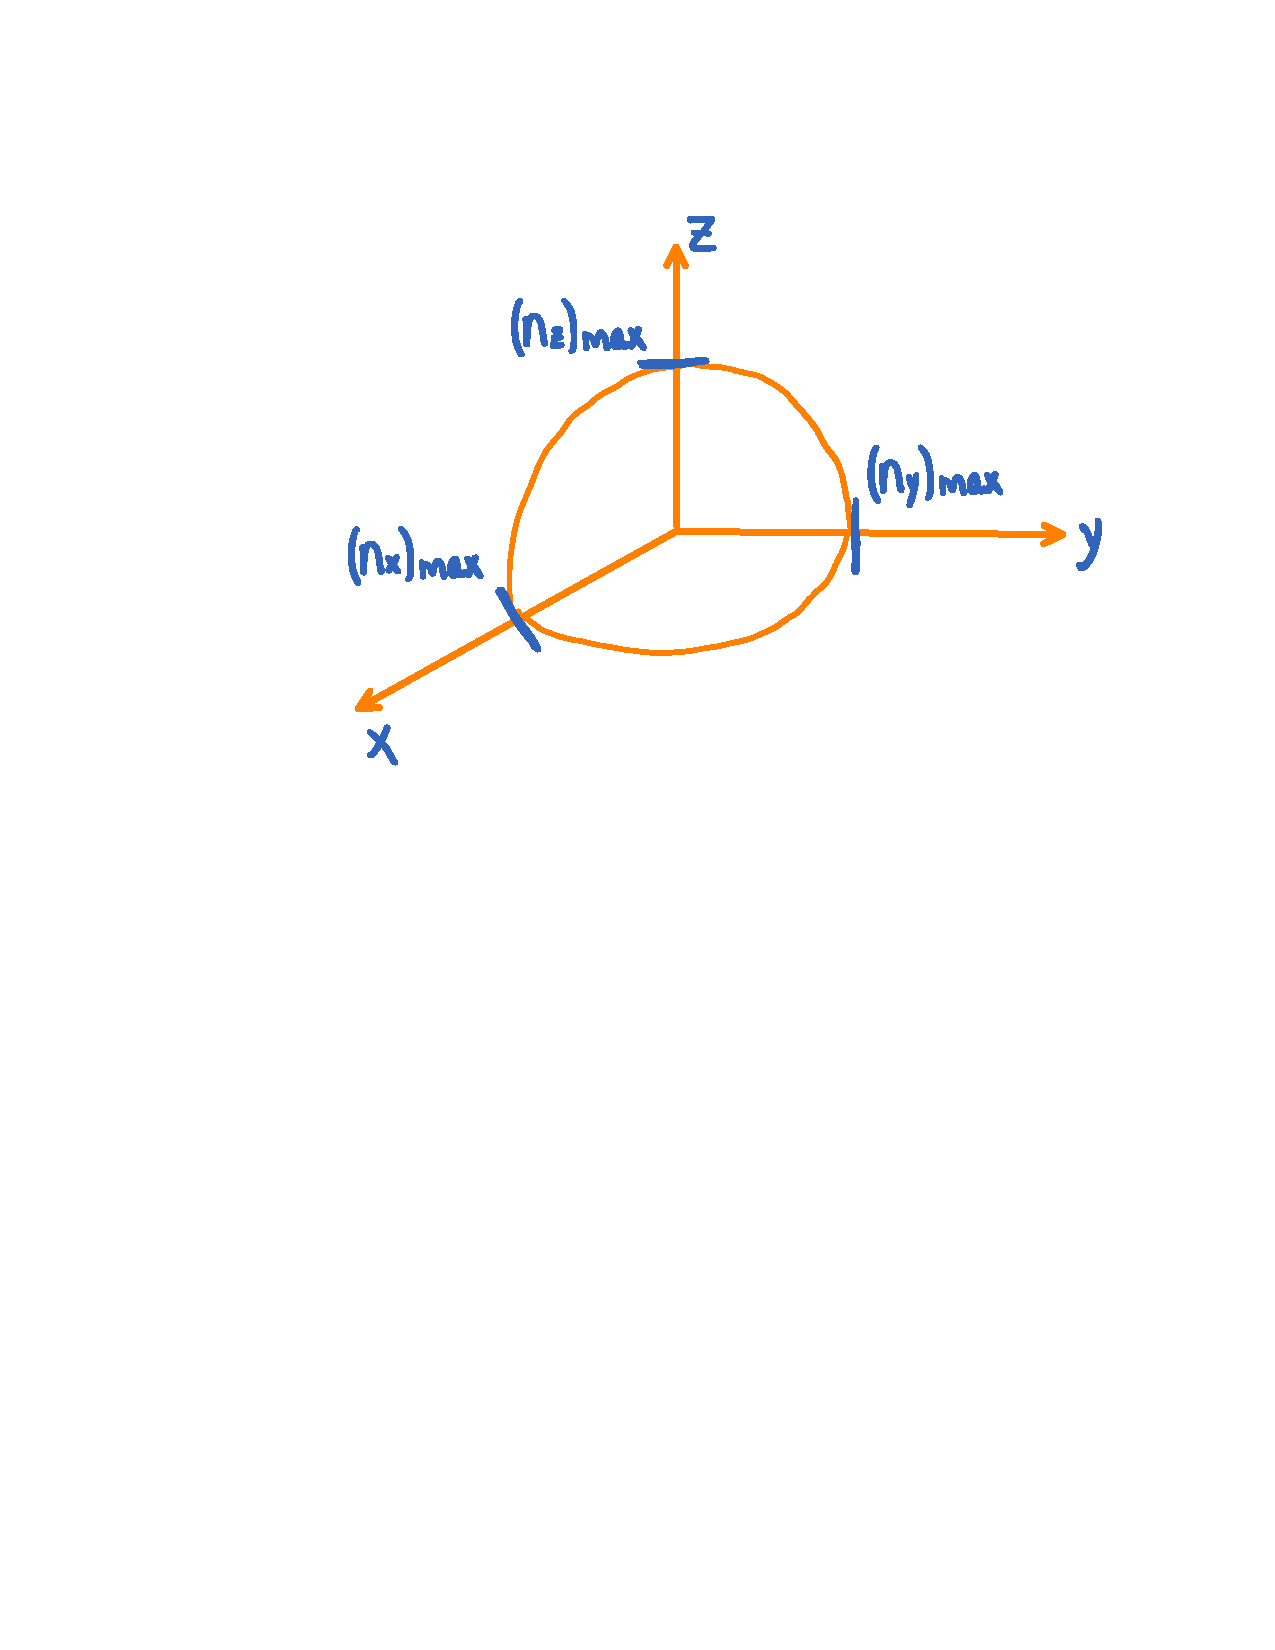
\includegraphics[scale=0.5]{octant.pdf}
\end{center}
Note here we only need to consider positive $n_x$, $n_y$, and $n_z$ by the parity of the equation (PSI). We want to find total number of states with energy less than or equal to $\hbar \omega$, which are states that lie in one octant of an ellipsoid whose axes are given by $(n_x)_{\max}$, $(n_y)_{\max}$, $(n_z)_{\max}$. To find $(n_x)_{\max}$, we write the following:
\begin{align*}
\omega = c\pi \frac{(n_x)_{\max}}{L_x} \qquad \Rightarrow \qquad (n_x)_{\max} = \frac{\omega L_x}{c \pi}
\end{align*}
Similarly, we have:
\begin{align*}
(n_y)_{\max} = \frac{\omega L_y}{c\pi} \qquad\qquad\qquad (n_z)_{\max} = \frac{\omega L_z}{c\pi}
\end{align*}
The number of states for each polarization with frequency less than or equal to $\omega$ is given by:
\begin{align*}
\text{Number of states for each polarization} &= \frac{1}{8} \cdot \text{Volume of the ellipsoid} \\&= \frac{1}{8}\cdot  \left( \frac{4\pi}{3}\right)\cdot (n_x)_{\max} \cdot (n_y)_{\max}\cdot (n_z)_{\max}\\
&= \frac{1}{8}\left( \frac{4\pi}{3}\right)\left( \frac{\omega L_x}{c\pi}\right)\left( \frac{\omega L_y}{c\pi}\right)\left( \frac{\omega L_z}{c\pi}\right)\\
&= \frac{1}{6\pi^2}\frac{\omega^3}{c^2} L_xL_yyL_z\\
&= \frac{1}{6\pi^2}\frac{\omega^3}{c^2} V
\end{align*}
For two polarizations, the total number of state with frequency less than or equal to $\omega$ is given by:
\begin{align*}
\text{Total number of states} = \frac{2}{6\pi^2}\frac{\omega^3}{c^2} L_xL_yyL_z = \frac{1}{3\pi^2}\frac{\omega^3}{c^2} V
\end{align*}
Even though we use a particular boundary condition, this is true for general periodic condition. \\

So the number of orbitals in frequency range between $\omega$ and $\omega+d\omega$ is given by the following:
\begin{align*}
d\that{n} = \frac{1}{3\pi^2} \frac{V}{c^3} \omega^2 \, d\omega
\end{align*}
The number of orbitals in frequency range between $\omega$ and $\omega+d\omega$ per unit volume is given by:
\begin{align*}
dn = \frac{1}{\pi^2}\frac{\omega^2}{c^3}\, d\omega
\end{align*}
Here each orbital has a mean number of photon given by:
\begin{align*}
\bar{n}(\omega) = \frac{1}{e^{\beta \hbar\omega} - 1}
\end{align*}
Each photon with frequency $\omega$ has energy $\hbar \omega$, putting all together, the mean radiation energy per unit volume in the energy range $\omega +d\omega$ is given by:
\begin{align*}
\bar{u}(\omega, T) \, d\omega = \left( \frac{1}{\pi^2}\frac{\omega^2 d\omega}{c^3}\right) (\hbar \omega)\left(\frac{1}{e^{\frac{\hbar \omega}{kT}} - 1 } \right)=\frac{\hbar}{\pi^2 c^3} \frac{\omega^3 \, d\omega}{e^{\frac{\hbar \omega}{kT}}-1} \tag{PR}
\end{align*}
and here $\bar{u}$ gives the radiation energy per unit volume per unit frequency range, and equation (PR) is the Plank's radiation formula derived using Bozon statistics.\\


%Given the energies $\epsilon_r$ for each state for each photon, to describe photon orbitals, we write:
%\begin{align*}
%\bar{E} = \sum_r \bar{n}_r \epsilon_r
%\end{align*}
%Recall that we have $\epsilon_r =\hbar \omega_r$. Photons form standing waves. \\

By Plank's Law for small $\omega$, we have $\hbar \omega << kT$, and hence $e^{\frac{\hbar \omega}{kT}}-1 \approx \frac{\hbar \omega}{kT}$, then we get:
\begin{align*}
\bar{u}(\omega, T ) \, d\omega = \frac{\hbar}{\pi^2 c^3} \frac{\omega^3 d\omega}{\frac{\hbar \omega}{kT}} = kT \frac{\omega^2 d\omega}{\pi^2 c^3} = kT \, dn \tag{RL}
\end{align*}
Equation (RL) is the expected result from the Equipartition Theorem, and this is called the Rayleigh-Jeans Law, which fails when frequency gets large.\\
\begin{center}
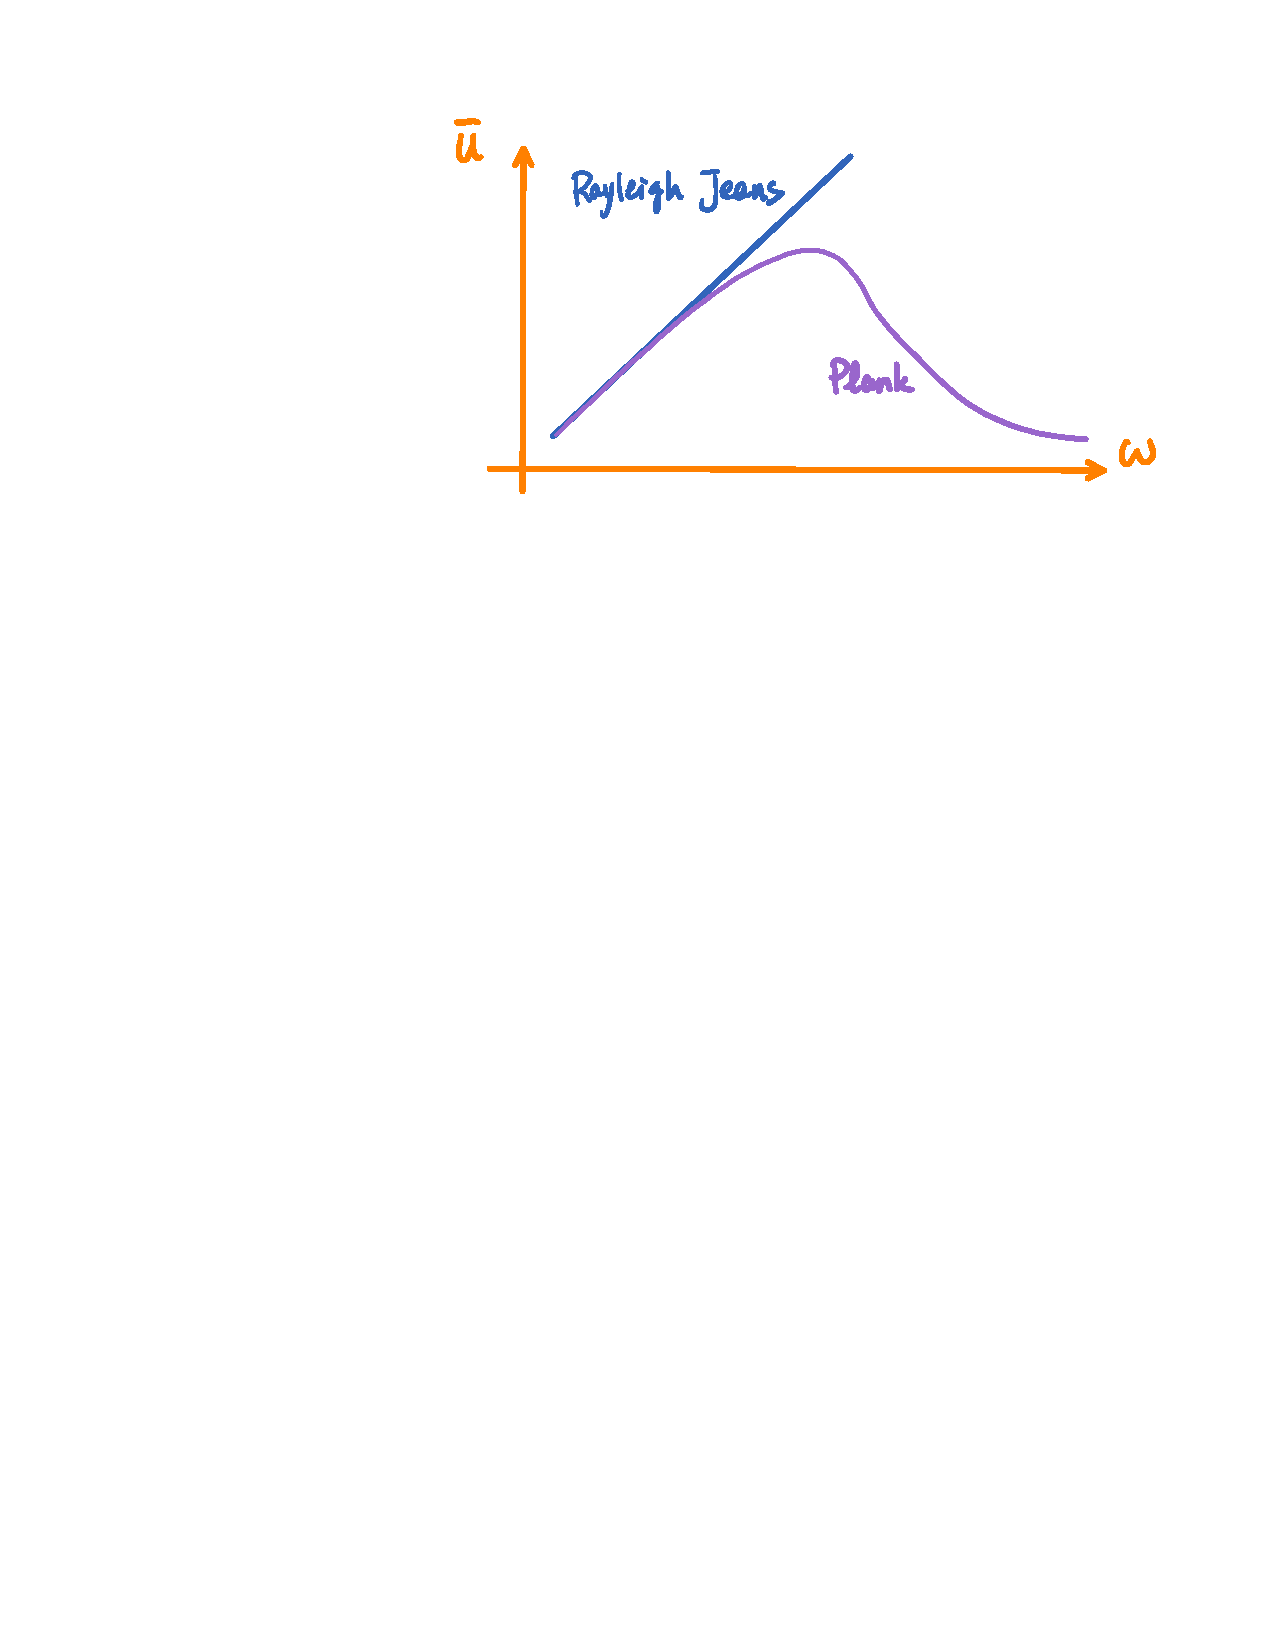
\includegraphics[scale=0.69]{RJ.pdf}
\end{center}

\newpage
Under equation (PR), note that the maximum of $\bar{u}(\omega, T)$ occurs at some $\omega = \that{\omega}$ given by:
\begin{align*}
\left. \frac{d\bar{u}}{d\omega}\right|_{\omega = \that{\omega}} = 0 \qquad \Rightarrow \qquad \that{\omega}\text{ is proportional to }T \ \ \that{\omega} = \frac{3kT}{\hbar}
\end{align*}
Hence we have the following at different temperature $T_1$ and $T_2$ with maximized $\that{\omega}_1$ and $\that{\omega}_2$:
\begin{align*}
\frac{\that{\omega}_1}{T_1} = \frac{\that{\omega}_2}{T_2}
\end{align*}
which gives the Wein's Displacement Law. \\

\begin{center}
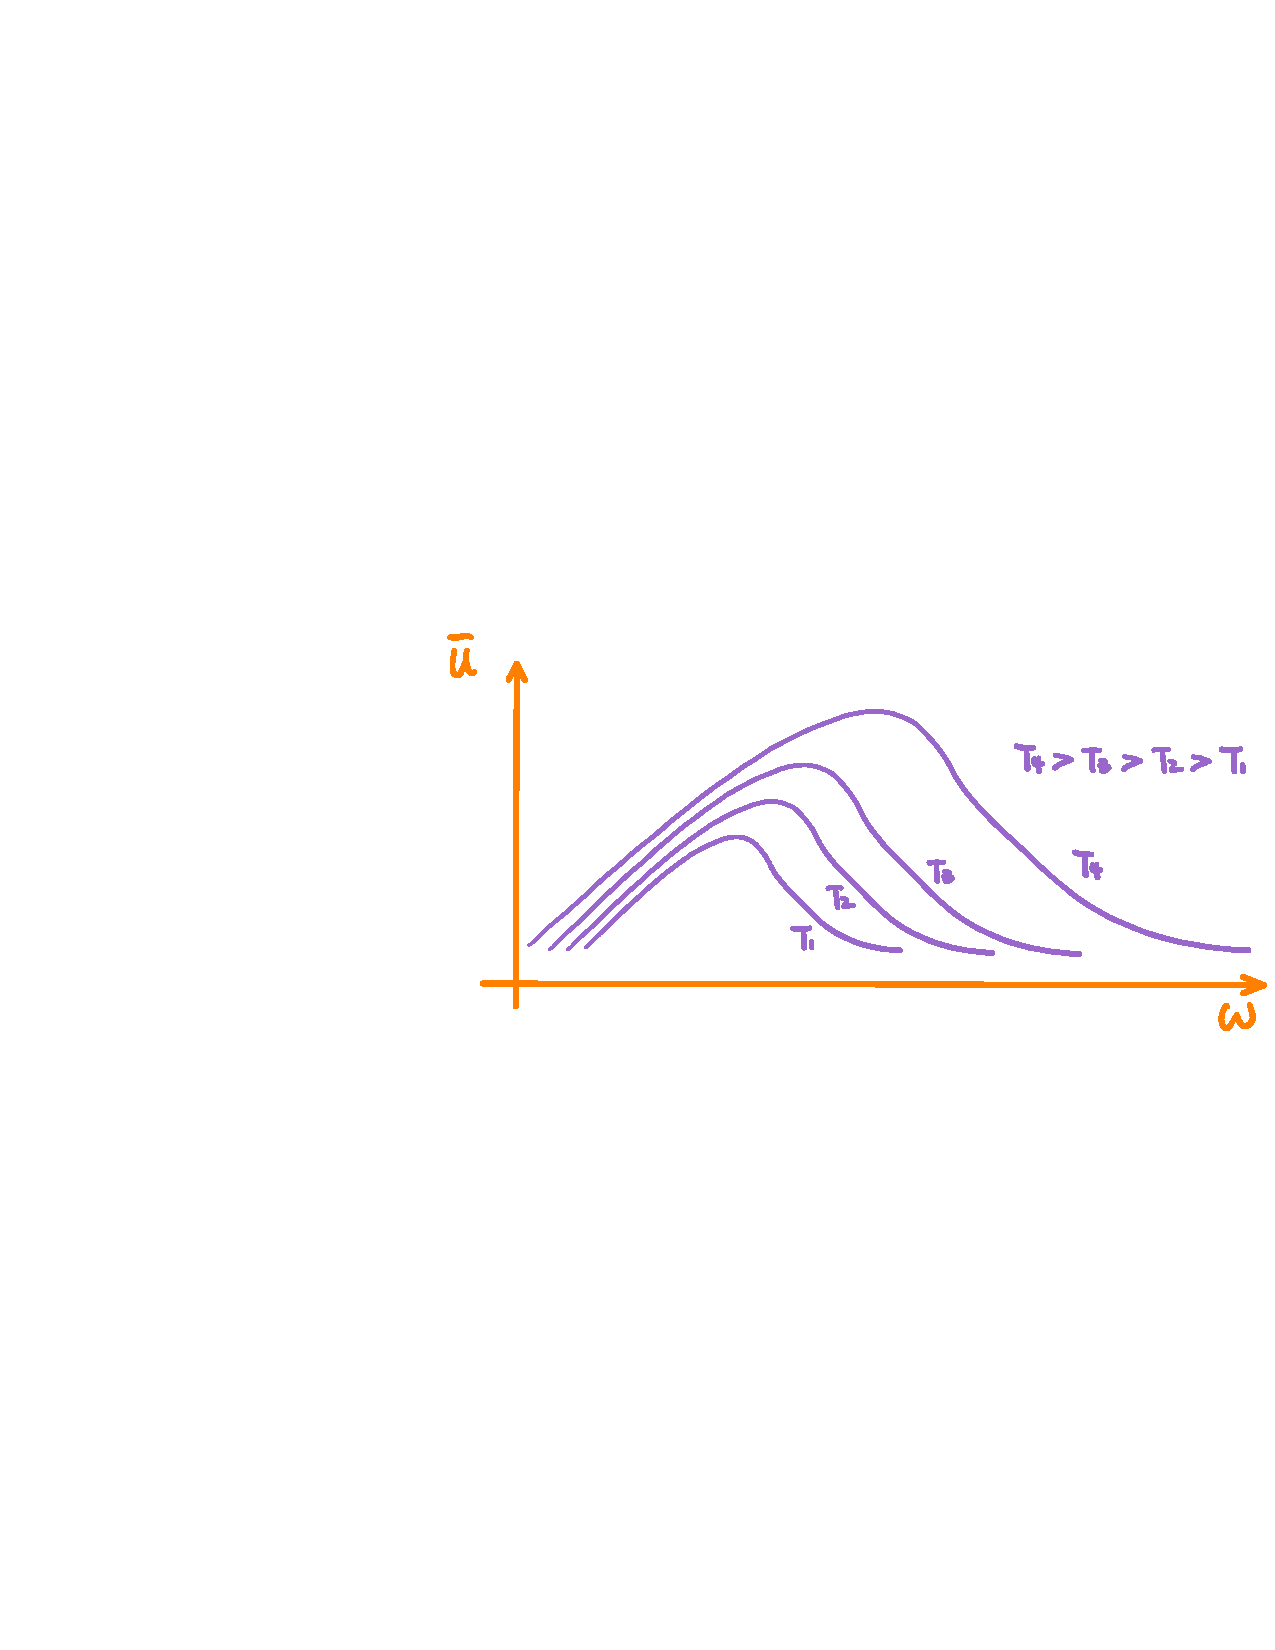
\includegraphics[scale=0.69]{Plank.pdf}
\end{center}

Now we will find the total energy density at a temperature $T$, we write the following:
\begin{align*}
\bar{u}_0(T) = \int_0^\infty \bar{u}(\omega, T) \, d\omega = \frac{\hbar}{\pi^2 c^3}\int_0^\infty \frac{\omega^3 \, d\omega}{e^{\frac{\hbar\omega}{kT}}-1} = \frac{\hbar}{\pi^2 c^3}\left( \frac{kT}{\hbar}\right)^4 \int_0^\infty \frac{x^3\, dx}{e^x - 1}
\end{align*}
where we set $x = \frac{\hbar \omega}{kT}$, and here $\int_0^\infty \frac{x^3\, dx}{e^x - 1} = \frac{\pi^4}{15}$. Combining we get:
\begin{align*}
\bar{u}_0(T) = \frac{\hbar}{\pi^2 c^3}\left( \frac{kT}{\hbar}\right)^4 \frac{\pi^4}{15} = \frac{\pi^2}{15} \frac{(kT)^4}{(\hbar c)^3}
\end{align*}
Here we see clearly that we have the relationship:
\begin{align*}
\bar{u}_0\propto T^4 
\end{align*}
which is called the Stefan-Boltzmann law. 

\newpage
\section[Effusion of a Photon Gas]{\color{red}Effusion of a Photon Gas\color{black}}
Consider a photon gas striking a wall.
\begin{center}
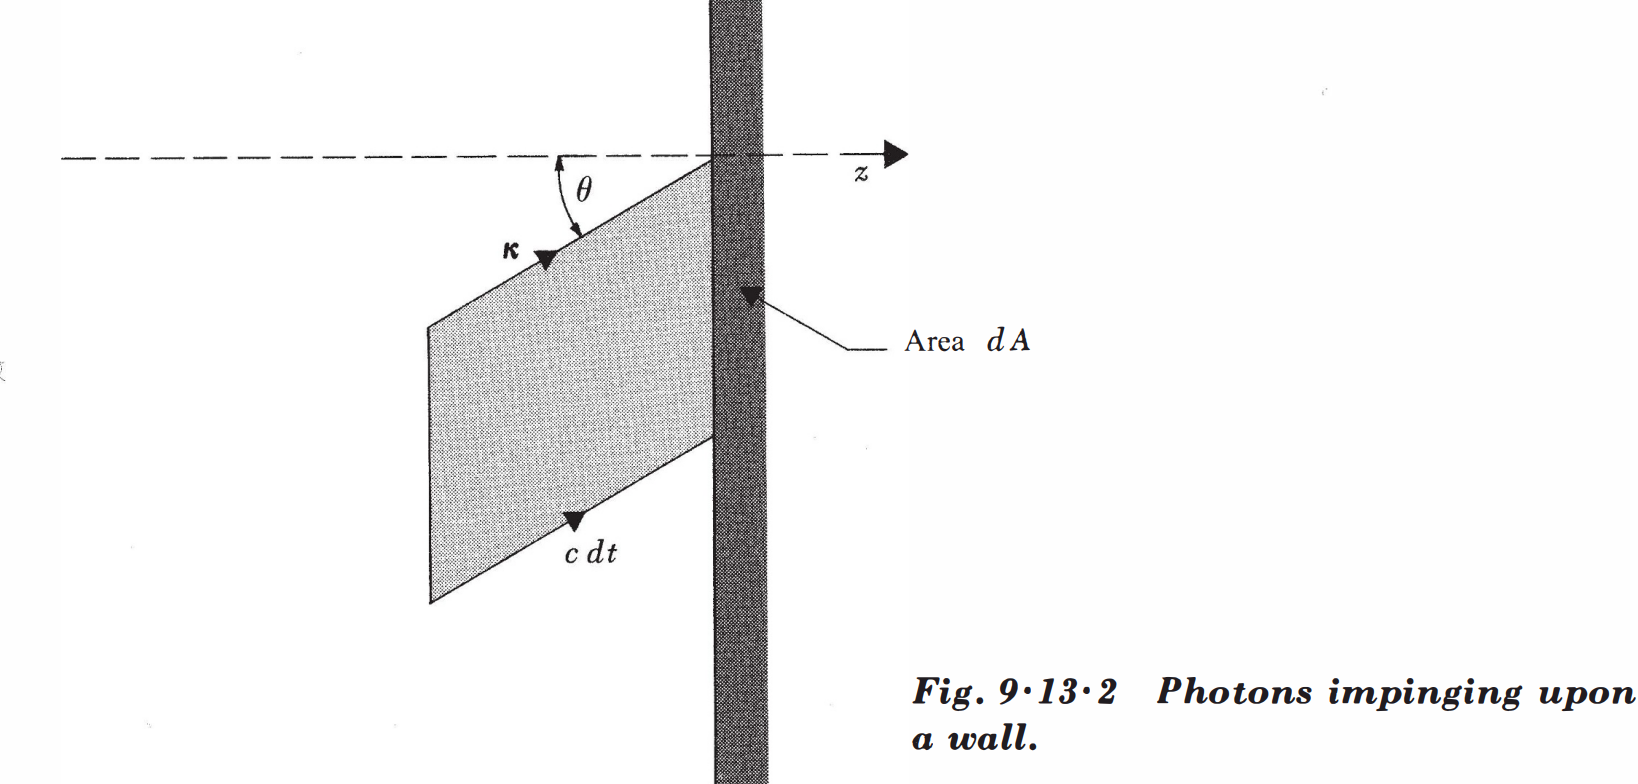
\includegraphics[scale=0.35]{photonEffu.png}
\end{center}
All photons in cylinder described above, with height $c \cos(\theta)\, dt$ strikes area $dA$ in time $dt$. All photon have same speed $c$, so do not need to worry about speed distribution. So the energy flux per unit area due to photons of given $\omega $ striking $dA$ at an angle $\theta$ as shown is given by the following:
\begin{align*}
\frac{(\text{Energy per unit volume})\cdot (c\cos(\theta) \, dA \, dt)}{dA\, dt} =\bar{u}\,c \cos(\theta)
\end{align*}
Note that photons are equally likely to go in any direction, so we need to average overall directions with $\cos(\theta) > 0$, where we get:
\begin{align*}
\overline{c\cos(\theta)} &= \frac{\int_{\cos(\theta)>0} c\cos(\theta)\, d\Omega}{\int_{\text{all }\theta} d\Omega} \\
&= \frac{\int_0^{\pi/2} c\cos(\theta) (2\pi \sin(\theta))\, d\theta}{4\pi} \\
&= \frac{c}{2}\int_0^{\pi/2} \cos(\theta)\sin(\theta) \, d\theta = \frac{c}{4}\int_0^{\pi/2} \sin(2\theta)\, d\theta \\
&= \frac{c}{4}
\end{align*}
Energy flux per unit area for given $\omega$, denoted as $\Phi(\omega)$, is then given by the following:
\begin{align*}
\Phi(\omega) = \frac{c\bar{u}}{4} 
\end{align*}
The total energy flux per unit area, or the power of radiation per unit area, is given by the following:
\begin{align*}
\text{Power of radiation per unit area} = \int_0^{\infty }\Phi(\omega)\, d\omega = \frac{c\bar{u}_0(T)}{4} = \frac{c}{4} \frac{\pi^2}{15} \frac{k^4T^4}{c^2 \hbar^3} \coloneqq \sigma T^4
\end{align*}
where $\sigma = \frac{\pi^2}{60}\frac{k^4}{c^3 \hbar^3}$ is called the Stefan Boltzmann constant. \\

\newpage
\section[Pressure of a Photon Gas]{\color{red}Pressure of a Photon Gas\color{black}}
For any photon orbital, we have $\epsilon_r = \hbar \omega_r = hc\pi \left( \frac{n_x^2}{L_x^2} + \frac{n_y^2}{L_y^2} + \frac{n_z^2}{L_z^2}\right)^{1/2}$, hence the force of a photon in orbital $r$ striking on a wall perpendicular to the $x$-axis is given by:
\begin{align*}
(F_x)_r = -\frac{\partial \epsilon_r}{\partial L_x} = -\hbar c\pi \frac{1}{2}\left( \frac{n_x^2}{L_x^2} + \frac{n_y^2}{L_y^2} + \frac{n_z^2}{L_z^2} \right)^{-1/2} \left( -\frac{2n_x^2}{L_x^3}\right)
\end{align*}
So pressure on wall of area $L_yL_z$ is given by:
\begin{align*}
\left( p_x\right)_r = \hbar c\pi \left(  \frac{n_x^2}{L_x^2} + \frac{n_y^2}{L_y^2} + \frac{n_z^2}{L_z^2}\right)^{-1/2} \frac{n_x^2}{L_x^2}\frac{1}{L_xL_yL_z}
\end{align*}
One can obtain $( p_y)_r$ and $(p_z)_r$ similarly, combining we get:
\begin{align*}
(p_x+p_y+p_z)_r = \hbar c\pi \left( \frac{n_x^2}{L_x^2} + \frac{n_y^2}{L_y^2} + \frac{n_z^2}{L_z^2} \right)^{-1/2}\left(  \frac{n_x^2}{L_x^2} + \frac{n_y^2}{L_y^2} + \frac{n_z^2}{L_z^2}\right) \frac{1}{L_xL_yL_z} = \frac{\epsilon_r}{V}
\end{align*}
Average over all orbitals, we get:
\begin{align*}
\overline{(p_x+p_y+p_z)} = 3\bar{p} = \frac{\overline{\epsilon_r}}{V} = \bar{u}_0 \qquad \Rightarrow \qquad \bar{p} = \frac{1}{3}\bar{u}_0
\end{align*}

\end{document}
